 %%%%%%%%%%%%%%%%%%%%%%%%%%%%%%%%%%%%%%%%%%%%%%%%%%%%%%%%%%%%%%%%%%%%%%
% Template for a UBC-compliant dissertation
% At the minimum, you will need to change the information found
% after the "Document meta-data"
%
%!TEX TS-program = pdflatex
%!TEX encoding = UTF-8 Unicode

%% The ubcdiss class provides several options:
%%   gpscopy (aka fogscopy)
%%       set parameters to exactly how GPS specifies
%%         * single-sided
%%         * page-numbering starts from title page
%%         * the lists of figures and tables have each entry prefixed
%%           with 'Figure' or 'Table'
%%       This can be tested by `\ifgpscopy ... \else ... \fi'
%%   10pt, 11pt, 12pt
%%       set default font size
%%   oneside, twoside
%%       whether to format for single-sided or double-sided printing
%%   balanced
%%       when double-sided, ensure page content is centred
%%       rather than slightly offset (the default)
%%   singlespacing, onehalfspacing, doublespacing
%%       set default inter-line text spacing; the ubcdiss class
%%       provides \textspacing to revert to this configured spacing
%%   draft
%%       disable more intensive processing, such as including
%%       graphics, etc.
%%

% For submission to GPS
\documentclass[gpscopy,oneside,onehalfspacing,11pt]{ubcdiss}

% For your own copies (looks nicer)
% \documentclass[balanced,twoside,11pt]{ubcdiss}

%%%%%%%%%%%%%%%%%%%%%%%%%%%%%%%%%%%%%%%%%%%%%%%%%%%%%%%%%%%%%%%%%%%%%%
%%%%%%%%%%%%%%%%%%%%%%%%%%%%%%%%%%%%%%%%%%%%%%%%%%%%%%%%%%%%%%%%%%%%%%
%%
%% FONTS:
%% 
%% The defaults below configures Times Roman for the serif font,
%% Helvetica for the sans serif font, and Courier for the
%% typewriter-style font.  Configuring fonts can be time
%% consuming; we recommend skipping to END FONTS!
%% 
%% If you're feeling brave, have lots of time, and wish to use one
%% your platform's native fonts, see the commented out bits below for
%% XeTeX/XeLaTeX.  This is not for the faint at heart. 
%% (And shouldn't you be writing? :-)
%%

%% NFSS font specification (New Font Selection Scheme)
\usepackage{times,mathptmx,courier}
\usepackage[scaled=.92]{helvet}

%% Math or theory people may want to include the handy AMS macros
\usepackage{amssymb}
\usepackage{amsmath}
\usepackage{amsfonts}

%% The pifont package provides access to the elements in the dingbat font.   
%% Use \ding{##} for a particular dingbat (see p7 of psnfss2e.pdf)
%%   Useful:
%%     51,52 different forms of a checkmark
%%     54,55,56 different forms of a cross (saltyre)
%%     172-181 are 1-10 in open circle (serif)
%%     182-191 are 1-10 black circle (serif)
%%     192-201 are 1-10 in open circle (sans serif)
%%     202-211 are 1-10 in black circle (sans serif)
%% \begin{dinglist}{##}\item... or dingautolist (which auto-increments)
%% to create a bullet list with the provided character.
\usepackage{pifont}

%%%%%%%%%%%%%%%%%%%%%%%%%%%%%%%%%%%%%%%%%%%%%%%%%%%%%%%%%%%%%%%%%%%%%%
%% Configure fonts for XeTeX / XeLaTeX using the fontspec package.
%% Be sure to check out the fontspec documentation.
%\usepackage{fontspec,xltxtra,xunicode}	% required
%\defaultfontfeatures{Mapping=tex-text}	% recommended
%% Minion Pro and Myriad Pro are shipped with some versions of
%% Adobe Reader.  Adobe representatives have commented that these
%% fonts can be used outside of Adobe Reader.
%\setromanfont[Numbers=OldStyle]{Minion Pro}
%\setsansfont[Numbers=OldStyle,Scale=MatchLowercase]{Myriad Pro}
%\setmonofont[Scale=MatchLowercase]{Andale Mono}

%% Other alternatives:
%\setromanfont[Mapping=tex-text]{Adobe Caslon}
%\setsansfont[Scale=MatchLowercase]{Gill Sans}
%\setsansfont[Scale=MatchLowercase,Mapping=tex-text]{Futura}
%\setmonofont[Scale=MatchLowercase]{Andale Mono}
%\newfontfamily{\SYM}[Scale=0.9]{Zapf Dingbats}
%% END FONTS
%%%%%%%%%%%%%%%%%%%%%%%%%%%%%%%%%%%%%%%%%%%%%%%%%%%%%%%%%%%%%%%%%%%%%%
%%%%%%%%%%%%%%%%%%%%%%%%%%%%%%%%%%%%%%%%%%%%%%%%%%%%%%%%%%%%%%%%%%%%%%

%%%%%%%%%%%%%%%%%%%%%%%%%%%%%%%%%%%%%%%%%%%%%%%%%%%%%%%%%%%%%%%%%%%%%%
%%%%%%%%%%%%%%%%%%%%%%%%%%%%%%%%%%%%%%%%%%%%%%%%%%%%%%%%%%%%%%%%%%%%%%
%%
%% My packages
%%

%% Caption on the right
%\usepackage{floatrow}

%% force figure position
\usepackage{float}

%% Aspect Ratio Symbol
\usepackage{ar}

%% typeset c++ code
\usepackage{listings}
\usepackage{xcolor}
\definecolor{dkgreen}{rgb}{0,0.6,0}
\definecolor{dred}{rgb}{0.545,0,0}
\definecolor{dblue}{rgb}{0,0,0.545}
\definecolor{lgrey}{rgb}{0.9,0.9,0.9}
\definecolor{gray}{rgb}{0.4,0.4,0.4}
\definecolor{darkblue}{rgb}{0.0,0.0,0.6}
\definecolor{lbcolor}{rgb}{0.85,0.85,0.85}
\lstdefinelanguage{cpp}{
      backgroundcolor=\color{white},  
      basicstyle=\footnotesize \ttfamily \color{black} \bfseries,   
      breakatwhitespace=false,       
      breaklines=true,               
      captionpos=b,                   
      commentstyle=\color{gray},   
      deletekeywords={...},          
      escapeinside={\%*}{*)},                  
      frame=single,                  
      language=C++,                
      keywordstyle=\color{purple},  
      morekeywords={BRIEFDescriptorConfig,string,TiXmlNode,DetectorDescriptorConfigContainer,istringstream,cerr,exit}, 
      identifierstyle=\color{black},
      stringstyle=\color{blue},      
      numbers=left,                 
      numbersep=5pt,                  
      numberstyle=\tiny\color{black}, 
      rulecolor=\color{black},        
      showspaces=false,               
      showstringspaces=false,        
      showtabs=false,                
      stepnumber=1,                   
      tabsize=5,                     
      title=\lstname,                 
    }

%\definecolor{listinggray}{gray}{0.9}
%\definecolor{lbcolor}{rgb}{0.9,0.9,0.9}
%\lstset{
%backgroundcolor=\color{lbcolor},
%    tabsize=4,    
%%   rulecolor=,
%    language=[GNU]C++,
%        basicstyle=\scriptsize,
%        upquote=true,
%        aboveskip={1.5\baselineskip},
%        columns=fixed,
%        showstringspaces=false,
%        extendedchars=false,
%        breaklines=true,
%        prebreak = \raisebox{0ex}[0ex][0ex]{\ensuremath{\hookleftarrow}},
%        frame=single,
%        numbers=left,
%        showtabs=false,
%        showspaces=false,
%        showstringspaces=false,
%        identifierstyle=\ttfamily,
%        keywordstyle=\color[rgb]{0,0,1},
%        commentstyle=\color[rgb]{0.026,0.112,0.095},
%        stringstyle=\color[rgb]{0.627,0.126,0.941},
%        numberstyle=\color[rgb]{0.205, 0.142, 0.73},
%%        \lstdefinestyle{C++}{language=C++,style=numbers}’.
%}
%\lstset{
%    backgroundcolor=\color{lbcolor},
%    tabsize=4,
%  language=C++,
%  captionpos=b,
%  tabsize=3,
%  frame=lines,
%  numbers=left,
%  numberstyle=\tiny,
%  numbersep=5pt,
%  breaklines=true,
%  showstringspaces=false,
%  basicstyle=\footnotesize,
%%  identifierstyle=\color{magenta},
%  keywordstyle=\color[rgb]{0,0,1},
%  commentstyle=\color{Darkgreen},
%  stringstyle=\color{red}
%  }

%% increase depth of showing section numbers
\setcounter{tocdepth}{4}
\setcounter{secnumdepth}{4}

%% Definitions
\newtheorem{definition}{Definition}    %% this does it

% color: add support for expressing colour models.  Grey can be used
% to great effect to emphasize other parts of a graphic or text.
\usepackage{xcolor}
\definecolor{greytext}{gray}{0.5}

%% url: for typesetting URLs and smart(er) hyphenation.
% typeset urls in sans-serif
\usepackage{url}
\urlstyle{sf} 

% tikz for creating graphics in latex
\usepackage{tikz}
\usetikzlibrary{calc, arrows.meta}

% Use the command \Set{ } to typeset sets.
\usepackage{braket}

% Bold math fonts
\usepackage{bm}

% Set the margins
\usepackage[left=1.25in,right=1in,top=1in,bottom=1in]{geometry}

% Go to the next line instead of indenting, for a new paragraph.
\usepackage[parfill]{parskip}


% Put subfigures iside figures
\usepackage{subcaption}

% input algorithms
\usepackage{algorithm}
\usepackage[noend]{algpseudocode}

% multi row for tables
\usepackage{multirow}

% A diagonal box inside a table cell
\usepackage{diagbox}

% Multirow in tables 
\usepackage{multirow}

% listings: useful support for including source code listings, with
% optional special keyword formatting.  The \lstset{} causes
% the text to be typeset in a smaller sans serif font, with
% proportional spacing.
\usepackage{listings}
\lstset{basicstyle=\ttfamily\footnotesize,showstringspaces=false,fontadjust}

% For list of abbreviations
\usepackage{enumitem}

%%%%%%%%%%%%%%%%%%%%%%%%%%%%%%%%%%%%%%%%%%%%%%%%%%%%%%%%%%%%%%%%%%%%%%
%%%%%%%%%%%%%%%%%%%%%%%%%%%%%%%%%%%%%%%%%%%%%%%%%%%%%%%%%%%%%%%%%%%%%%



%%%%%%%%%%%%%%%%%%%%%%%%%%%%%%%%%%%%%%%%%%%%%%%%%%%%%%%%%%%%%%%%%%%%%%
%%%%%%%%%%%%%%%%%%%%%%%%%%%%%%%%%%%%%%%%%%%%%%%%%%%%%%%%%%%%%%%%%%%%%%
%%
%% Recommended packages
%%
\usepackage{checkend}	% better error messages on left-open environments
\usepackage{graphicx}	% for incorporating external images

%% booktabs: provides some special commands for typesetting tables as used
%% in excellent journals.  Ignore the examples in the Lamport book!
\usepackage{booktabs}

%% listings: useful support for including source code listings, with
%% optional special keyword formatting.  The \lstset{} causes
%% the text to be typeset in a smaller sans serif font, with
%% proportional spacing.
\usepackage{listings}
\lstset{basicstyle=\sffamily\scriptsize,showstringspaces=false,fontadjust}

%% The acronym package provides support for defining acronyms, providing
%% their expansion when first used, and building glossaries.  See the
%% example in glossary.tex and the example usage throughout the example
%% document.
%% NOTE: to use \MakeTextLowercase in the \acsfont command below,
%%   we *must* use the `nohyperlinks' option -- it causes errors with
%%   hyperref otherwise.  See Section 5.2 in the ``LaTeX 2e for Class
%%   and Package Writers Guide'' (clsguide.pdf) for details.
\usepackage[printonlyused,nohyperlinks]{acronym}
%% The ubcdiss.cls loads the `textcase' package which provides commands
%% for upper-casing and lower-casing text.  The following causes
%% the acronym package to typeset acronyms in small-caps
%% as recommended by Bringhurst.
\renewcommand{\acsfont}[1]{{\scshape \MakeTextLowercase{#1}}}

%% color: add support for expressing colour models.  Grey can be used
%% to great effect to emphasize other parts of a graphic or text.
%% For an excellent set of examples, see Tufte's "Visual Display of
%% Quantitative Information" or "Envisioning Information".
\usepackage{color}
\definecolor{greytext}{gray}{0.5}

%% comment: provides a new {comment} environment: all text inside the
%% environment is ignored.
%%   \begin{comment} ignored text ... \end{comment}
\usepackage{comment}

%% The natbib package provides more sophisticated citing commands
%% such as \citeauthor{} to provide the author names of a work,
%% \citet{} to produce an author-and-reference citation,
%% \citep{} to produce a parenthetical citation.
%% We use \citeeg{} to provide examples
\usepackage[numbers,sort&compress]{natbib}
\newcommand{\citeeg}[1]{\citep[e.g.,][]{#1}}

%% The titlesec package provides commands to vary how chapter and
%% section titles are typeset.  The following uses more compact
%% spacings above and below the title.  The titleformat that follow
%% ensure chapter/section titles are set in singlespace.
\usepackage[compact]{titlesec}
\titleformat*{\section}{\singlespacing\raggedright\bfseries\Large}
\titleformat*{\subsection}{\singlespacing\raggedright\bfseries\large}
\titleformat*{\subsubsection}{\singlespacing\raggedright\bfseries}
\titleformat*{\paragraph}{\singlespacing\raggedright\itshape}

%% The caption package provides support for varying how table and
%% figure captions are typeset.
\usepackage[format=hang,indention=-1cm,labelfont={bf},margin=1em]{caption}

%% url: for typesetting URLs and smart(er) hyphenation.
%% \url{http://...} 
\usepackage{url}
\urlstyle{sf}	% typeset urls in sans-serif


%%%%%%%%%%%%%%%%%%%%%%%%%%%%%%%%%%%%%%%%%%%%%%%%%%%%%%%%%%%%%%%%%%%%%%
%%%%%%%%%%%%%%%%%%%%%%%%%%%%%%%%%%%%%%%%%%%%%%%%%%%%%%%%%%%%%%%%%%%%%%
%%
%% Possibly useful packages: you may need to explicitly install
%% these from CTAN if they aren't part of your distribution;
%% teTeX seems to ship with a smaller base than MikTeX and MacTeX.
%%
%\usepackage{pdfpages}	% insert pages from other PDF files
%\usepackage{longtable}	% provide tables spanning multiple pages
%\usepackage{chngpage}	% support changing the page widths on demand
%\usepackage{tabularx}	% an enhanced tabular environment

%% enumitem: support pausing and resuming enumerate environments.
%\usepackage{enumitem}

%% rotating: provides two environments, sidewaystable and sidewaysfigure,
%% for typesetting tables and figures in landscape mode.  
%\usepackage{rotating}

%% subfig: provides for including subfigures within a figure,
%% and includes being able to separately reference the subfigures.
%\usepackage{subfig}

%% ragged2e: provides several new new commands \Centering, \RaggedLeft,
%% \RaggedRight and \justifying and new environments Center, FlushLeft,
%% FlushRight and justify, which set ragged text and are easily
%% configurable to allow hyphenation.
%\usepackage{ragged2e}

%% The ulem package provides a \sout{} for striking out text and
%% \xout for crossing out text.  The normalem and normalbf are
%% necessary as the package messes with the emphasis and bold fonts
%% otherwise.
%\usepackage[normalem,normalbf]{ulem}    % for \sout

%%%%%%%%%%%%%%%%%%%%%%%%%%%%%%%%%%%%%%%%%%%%%%%%%%%%%%%%%%%%%%%%%%%%%%
%% HYPERREF:
%% The hyperref package provides for embedding hyperlinks into your
%% document.  By default the table of contents, references, citations,
%% and footnotes are hyperlinked.
%%
%% Hyperref provides a very handy command for doing cross-references:
%% \autoref{}.  This is similar to \ref{} and \pageref{} except that
%% it automagically puts in the *type* of reference.  For example,
%% referencing a figure's label will put the text `Figure 3.4'.
%% And the text will be hyperlinked to the appropriate place in the
%% document.
%%
%% Generally hyperref should appear after most other packages

%% The following puts hyperlinks in very faint grey boxes.
%% The `pagebackref' causes the references in the bibliography to have
%% back-references to the citing page; `backref' puts the citing section
%% number.  See further below for other examples of using hyperref.
%% 2009/12/09: now use `linktocpage' (Jacek Kisynski): GPS now prefers
%%   that the ToC, LoF, LoT place the hyperlink on the page number,
%%   rather than the entry text.
\usepackage[bookmarks,bookmarksnumbered,%
    allbordercolors={0.8 0.8 0.8},%
    pagebackref,linktocpage%
    ]{hyperref}
%% The following change how the the back-references text is typeset in a
%% bibliography when `backref' or `pagebackref' are used
%%
%% Change \nocitations if you'd like some text shown where there
%% are no citations found (e.g., pulled in with \nocite{xxx})
\newcommand{\nocitations}{\relax}
%%\newcommand{\nocitations}{No citations}
%%
%\renewcommand*{\backref}[1]{}% necessary for backref < 1.33
\renewcommand*{\backrefsep}{,~}%
\renewcommand*{\backreftwosep}{,~}% ', and~'
\renewcommand*{\backreflastsep}{,~}% ' and~'
\renewcommand*{\backrefalt}[4]{%
\textcolor{greytext}{\ifcase #1%
\nocitations%
\or
\(\rightarrow\) page #2%
\else
\(\rightarrow\) pages #2%
\fi}}



%% The following uses most defaults, which causes hyperlinks to be
%% surrounded by colourful boxes; the colours are only visible in
%% PDFs and don't show up when printed:
%\usepackage[bookmarks,bookmarksnumbered]{hyperref}

%% The following disables the colourful boxes around hyperlinks.
%\usepackage[bookmarks,bookmarksnumbered,pdfborder={0 0 0}]{hyperref}

%% The following disables all hyperlinking, but still enabled use of
%% \autoref{}
%\usepackage[draft]{hyperref}

%% The following commands causes chapter and section references to
%% uppercase the part name.
\renewcommand{\chapterautorefname}{Chapter}
\renewcommand{\sectionautorefname}{Section}
\renewcommand{\subsectionautorefname}{Section}
\renewcommand{\subsubsectionautorefname}{Section}

%% If you have long page numbers (e.g., roman numbers in the 
%% preliminary pages for page 28 = xxviii), you might need to
%% uncomment the following and tweak the \@pnumwidth length
%% (default: 1.55em).  See the tocloft documentation at
%% http://www.ctan.org/tex-archive/macros/latex/contrib/tocloft/
% \makeatletter
% \renewcommand{\@pnumwidth}{3em}
% \makeatother

%%%%%%%%%%%%%%%%%%%%%%%%%%%%%%%%%%%%%%%%%%%%%%%%%%%%%%%%%%%%%%%%%%%%%%
%%%%%%%%%%%%%%%%%%%%%%%%%%%%%%%%%%%%%%%%%%%%%%%%%%%%%%%%%%%%%%%%%%%%%%
%%
%% Some special settings that controls how text is typeset
%%
% \raggedbottom		% pages don't have to line up nicely on the last line
% \sloppy		% be a bit more relaxed in inter-word spacing
% \clubpenalty=10000	% try harder to avoid orphans
% \widowpenalty=10000	% try harder to avoid widows
% \tolerance=1000

%% And include some of our own useful macros
% This file provides examples of some useful macros for typesetting
% dissertations.  None of the macros defined here are necessary beyond
% for the template documentation, so feel free to change, remove, and add
% your own definitions.
%
% We recommend that you define macros to separate the semantics
% of the things you write from how they are presented.  For example,
% you'll see definitions below for a macro \file{}: by using
% \file{} consistently in the text, we can change how filenames
% are typeset simply by changing the definition of \file{} in
% this file.
% 
%% The following is a directive for TeXShop to indicate the main file
%%!TEX root = diss.tex

\newcommand{\NA}{\textsc{n/a}}	% for "not applicable"
\newcommand{\eg}{e.g.,\ }	% proper form of examples (\eg a, b, c)
\newcommand{\ie}{i.e.,\ }	% proper form for that is (\ie a, b, c)
\newcommand{\etal}{\emph{et al. }}

% Some useful macros for typesetting terms.
\newcommand{\file}[1]{\texttt{#1}}
\newcommand{\class}[1]{\texttt{#1}}
\newcommand{\latexpackage}[1]{\href{http://www.ctan.org/macros/latex/contrib/#1}{\texttt{#1}}}
\newcommand{\latexmiscpackage}[1]{\href{http://www.ctan.org/macros/latex/contrib/misc/#1.sty}{\texttt{#1}}}
\newcommand{\env}[1]{\texttt{#1}}
\newcommand{\BibTeX}{Bib\TeX}

% Define a command \doi{} to typeset a digital object identifier (DOI).
% Note: if the following definition raise an error, then you likely
% have an ancient version of url.sty.  Either find a more recent version
% (3.1 or later work fine) and simply copy it into this directory,  or
% comment out the following two lines and uncomment the third.
\DeclareUrlCommand\DOI{}
\newcommand{\doi}[1]{\href{http://dx.doi.org/#1}{\DOI{doi:#1}}}
%\newcommand{\doi}[1]{\href{http://dx.doi.org/#1}{doi:#1}}

% Useful macro to reference an online document with a hyperlink
% as well with the URL explicitly listed in a footnote
% #1: the URL
% #2: the anchoring text
\newcommand{\webref}[2]{\href{#1}{#2}\footnote{\url{#1}}}

% epigraph is a nice environment for typesetting quotations
\makeatletter
\newenvironment{epigraph}{%
	\begin{flushright}
	\begin{minipage}{\columnwidth-0.75in}
	\begin{flushright}
	\@ifundefined{singlespacing}{}{\singlespacing}%
    }{
	\end{flushright}
	\end{minipage}
	\end{flushright}}
\makeatother

% \FIXME{} is a useful macro for noting things needing to be changed.
% The following definition will also output a warning to the console
\newcommand{\FIXME}[1]{\typeout{**FIXME** #1}\textbf{[FIXME: #1]}}

% END


%%%%%%%%%%%%%%%%%%%%%%%%%%%%%%%%%%%%%%%%%%%%%%%%%%%%%%%%%%%%%%%%%%%%%%
%%%%%%%%%%%%%%%%%%%%%%%%%%%%%%%%%%%%%%%%%%%%%%%%%%%%%%%%%%%%%%%%%%%%%%
%%
%% Document meta-data: be sure to also change the \hypersetup information
%%

\title{Entire Domain Advancing Layer Surface Mesh (EDAMSurf) Generation}
%\subtitle{If you want a subtitle}

\author{Jasmeet Singh}
\previousdegree{B. Tech, Indian Institute of Technology (BHU), Varanasi, 2015}
%\previousdegree{M. Silly Walks, Another University, 1994}

% What is this dissertation for?
\degreetitle{Masters in Applied Science}

\institution{The University of British Columbia}
\campus{Vancouver}

\faculty{The Faculty of Graduate and Postdoctoral Studies}
\department{Mechanical Engineering}
\submissionmonth{December}
\submissionyear{2019}

% details of your examining committee
\examiningcommittee{Carl Ollivier-Gooch, Mechanical Engineering}{Supervisor}
\examiningcommittee{Jasmin Jelovica, Mechanincal Engineering}%
    {Supervisory Committee Member}
\examiningcommittee{Dana Grecov, Mechanical Engineering}{Supervisory Committee Member}
%\examiningcommittee{Magnus Monolith, Other Department}{Additional Examiner}

% details of your supervisory committee
%\supervisorycommittee{Ira Crater, Materials Engineering}%
%    {Supervisory Committee Member}
%\supervisorycommittee{Adeline Long, \textsc{CEO} of Aerial Machine
%    Transportation, Inc.}{Supervisory Committee Member}

%% hyperref package provides support for embedding meta-data in .PDF
%% files
\hypersetup{
  pdftitle={Change this title!  (DRAFT: \today)},
  pdfauthor={Johnny Canuck},
  pdfkeywords={Your keywords here}
}

%%%%%%%%%%%%%%%%%%%%%%%%%%%%%%%%%%%%%%%%%%%%%%%%%%%%%%%%%%%%%%%%%%%%%%
%%%%%%%%%%%%%%%%%%%%%%%%%%%%%%%%%%%%%%%%%%%%%%%%%%%%%%%%%%%%%%%%%%%%%%
%% 
%% The document content
%%

%% LaTeX's \includeonly commands causes any uses of \include{} to only
%% include files that are in the list.  This is helpful to produce
%% subsets of your thesis (e.g., for committee members who want to see
%% the dissertation chapter by chapter).  It also saves time by 
%% avoiding reprocessing the entire file.
%\includeonly{intro,conclusions}
%\includeonly{methodology2}

\begin{document}

%%%%%%%%%%%%%%%%%%%%%%%%%%%%%%%%%%%%%%%%%%%%%%%%%%
%% From Thesis Components: Tradtional Thesis
%% <http://www.grad.ubc.ca/current-students/dissertation-thesis-preparation/order-components>

% Preliminary Pages (numbered in lower case Roman numerals)
%    1. Title page (mandatory)
\maketitle

%    2. Committee page (mandatory): lists supervisory committee and,
%    if applicable, the examining committee
\makecommitteepage

%    3. Abstract (mandatory - maximum 350 words)
%% The following is a directive for TeXShop to indicate the main file
%%!TEX root = diss.tex

\chapter{Abstract}

Use of unstructured meshes in the simulation of a computational field to solve for a real world problem is ubiquitous. Specially, solving fluid flow over bodies like an airplane or a turbine computationally requires a well discretized domain, or a mesh around the surfaces of these bodies. In Computational Fluid Dynamic (CFD) simulations over these surfaces, the flow at the viscous-boundary layer of the surface is very important as the gradients in the normal direction of the flow are sharp and are orders of magnitude higher than the gradients in the tangential direction of the flow. Hence, resolving the flow field in the boundary layer is vital for accurate simulation results.

A plethora of 3D boundary layer mesh generation techniques start off from a discretization of the surface. A majority of these techniques either use surface inflation or iterative point placement normal to the surface to generate the advancing layer 3D mesh. Generating boundary layer meshes in 3D depends on the quality of the underlying surface discretization. We introduce a technique to generate advancing layer surface meshes which would improve the mesh generation pipline for 3D mesh generation. The technique takes an input triangulation of the surface, which is fairly easy to get, even for complex geometries. Surface segments are identified and these segmentsare meshed independently using a advancing-layer methodology. For each surface segment, a mesh is generated by advancing layers from the identified boundaries to the surface interior while deforming the existing triangulation. As the mesh-generation technique introduced here produces a closed-mesh, we get a valid mesh at each iteration of advancing layer.

The method introduced to generate advancing layer meshes 

A Viscous-boundary layer mesh generation technique based on advancing layer 

Fluid flow over an object is ubiquitous in real-world problems. Computational Fluid Dynamics (CFD) simulations try to reproduce the physics involved in such problems without the need of doing experiments. These simulations utilize the discretized domain around the object, also called a mesh to proceed with the solution. 

% Consider placing version information if you circulate multiple drafts
%\vfill
%\begin{center}
%\begin{sf}
%\fbox{Revision: \today}
%\end{sf}
%\end{center}

\cleardoublepage

%    4. Lay Summary (Effective May 2017, mandatory - maximum 150 words)
%% The following is a directive for TeXShop to indicate the main file
%%!TEX root = diss.tex

%% https://www.grad.ubc.ca/current-students/dissertation-thesis-preparation/preliminary-pages
%% 
%% LAY SUMMARY Effective May 2017, all theses and dissertations must
%% include a lay summary.  The lay or public summary explains the key
%% goals and contributions of the research/scholarly work in terms that
%% can be understood by the general public. It must not exceed 150
%% words in length.

\chapter{Lay Summary}

Discretization of geometries using a non-regular arrangement of mesh elements, called unstructured- mesh generation, is used widely for simulating flow over various objects in industry and government. The region near the surfaces of objects is particularly important during the simulation process because of the extreme non-linearity in the flow characteristics near the boundaries of objects. Hence, generating a well-discretized boundary layer mesh is key to superior flow simulation results. 3D mesh generation methodologies use a surface mesh as the starting point. Hence, the surface mesh plays an important role in the overall fluid flow simulation process.

A method to generate surface meshes which can be extended to three dimensions is demonstrated. The meshes produced will have improved ability to tackle boundary layer flows. Example meshes are produced which demonstrate the capabilities of the algorithm developed.

%The lay or public summary explains the key goals and contributions of the research/scholarly work in terms that can be understood by the general public. It must not exceed 150 words in length.

\cleardoublepage

%    5. Preface
%% The following is a directive for TeXShop to indicate the main file
%%!TEX root = diss.tex

\chapter{Preface}

At \ac{UBC}, a preface may be required.  Be sure to check the
\ac{GPS} guidelines as they may have specific content to be included.

\cleardoublepage

%    6. Table of contents (mandatory - list all items in the preliminary pages
%    starting with the abstract, followed by chapter headings and
%    subheadings, bibliographies and appendices)
\tableofcontents
\cleardoublepage	% required by tocloft package

%    7. List of tables (mandatory if thesis has tables)
\listoftables
\cleardoublepage	% required by tocloft package

%    8. List of figures (mandatory if thesis has figures)
\listoffigures
\cleardoublepage	% required by tocloft package

%    9. List of illustrations (mandatory if thesis has illustrations)
%   10. Lists of symbols, abbreviations or other (optional)

%   11. Glossary (optional)
%%% The following is a directive for TeXShop to indicate the main file
%%!TEX root = diss.tex

\chapter{Glossary}

This glossary uses the handy \latexpackage{acroynym} package to automatically
maintain the glossary.  It uses the package's \texttt{printonlyused}
option to include only those acronyms explicitly referenced in the
\LaTeX\ source.  To change how the acronyms are rendered, change the
\verb+\acsfont+ definition in \verb+diss.tex+.

% use \acrodef to define an acronym, but no listing
\acrodef{UI}{user interface}
\acrodef{UBC}{University of British Columbia}

% The acronym environment will typeset only those acronyms that were
% *actually used* in the course of the document
\begin{acronym}[ANOVA]
\acro{ANOVA}[ANOVA]{Analysis of Variance\acroextra{, a set of
  statistical techniques to identify sources of variability between groups}}
\acro{API}{application programming interface}
\acro{CTAN}{\acroextra{The }Common \TeX\ Archive Network}
\acro{DOI}{Document Object Identifier\acroextra{ (see
    \url{http://doi.org})}}
\acro{GPS}[GPS]{Graduate and Postdoctoral Studies}
\acro{PDF}{Portable Document Format}
\acro{RCS}[RCS]{Revision control system\acroextra{, a software
    tool for tracking changes to a set of files}}
\acro{TLX}[TLX]{Task Load Index\acroextra{, an instrument for gauging
  the subjective mental workload experienced by a human in performing
  a task}}
\acro{UML}{Unified Modelling Language\acroextra{, a visual language
    for modelling the structure of software artefacts}}
\acro{URL}{Unique Resource Locator\acroextra{, used to describe a
    means for obtaining some resource on the world wide web}}
\acro{W3C}[W3C]{\acroextra{the }World Wide Web Consortium\acroextra{,
    the standards body for web technologies}}
\acro{XML}{Extensible Markup Language}
\end{acronym}

% You can also use \newacro{}{} to only define acronyms
% but without explictly creating a glossary
% 
% \newacro{ANOVA}[ANOVA]{Analysis of Variance\acroextra{, a set of
%   statistical techniques to identify sources of variability between groups.}}
% \newacro{API}[API]{application programming interface}
% \newacro{GOMS}[GOMS]{Goals, Operators, Methods, and Selection\acroextra{,
%   a framework for usability analysis.}}
% \newacro{TLX}[TLX]{Task Load Index\acroextra{, an instrument for gauging
%   the subjective mental workload experienced by a human in performing
%   a task.}}
% \newacro{UI}[UI]{user interface}
% \newacro{UML}[UML]{Unified Modelling Language}
% \newacro{W3C}[W3C]{World Wide Web Consortium}
% \newacro{XML}[XML]{Extensible Markup Language}
	% always input, since other macros may rely on it

\textspacing		% begin one-half or double spacing

%   12. Acknowledgements (optional)
%% The following is a directive for TeXShop to indicate the main file
%%!TEX root = diss.tex

\chapter{Acknowledgments}

%I would like to acknowledge and thank all the people who were a part of my graduate degree at UBC. These include the professors who taught me in lectures, my classmates, my labmates, people in the broader graduate community with whom I met at various academic and social events, my friends and family.

%I would like to thank my supervisor, Dr. Carl Ollivier-Gooch. 

****************************************************************\\
To be updated \\
****************************************************************

%Thank those people who helped you. 

%Don't forget your parents or loved ones.

%You may wish to acknowledge your funding sources.


%   13. Dedication (optional)

% Body of Thesis (not all sections may apply)
\mainmatter

\acresetall	% reset all acronyms used so far

% Thesis outline
%%-----------------------------------------------------------------------------
% c0_outline.tex:
%     Thesis outline.         
%
%-----------------------------------------------------------------------------
\subsection*{Thesis Outline}

****************************************************************\\
Only for guidance right now, this page will be commented out. \\
****************************************************************

\begin{enumerate}
  \item Introduction
    \begin{itemize}
      \item Introduction to Meshing
      \item Introduction to unstructured meshing and its importance
      \item Boundary Layer Phenomenon and its importance
      \item Meshes that deal with such scenarios.
      \item 2D previous works
      \item 3D previous works
      \item Surface Mesh generation methods
        \begin{itemize}
          \item Parametric Mapping
          \item Direct 3D methods
        \end{itemize}
    \end{itemize}
  \item   
\end{enumerate}
%%% Local Variables:
%%% TeX-master: "diss"
%%% End:
\endinput

\cleardoublepage

%    1. Introduction
	%% The following is a directive for TeXShop to indicate the main file
%%!TEX root = diss.tex

\chapter{Introduction}
\label{ch:Introduction}

\begin{epigraph}
    \emph{If I have seen farther it is by standing on the shoulders of
    Giants.} ---~Sir Isaac Newton (1855)
\end{epigraph}

Computational Fluid Simulations (CFD) is a field of study where scientists and engineers architect new ways to numerically solve fluid flow equations. Before the advent of computers, numerical solutions of differential equations was done by hand. This lead to a great deal of work in the direction of creating faster algorithms to solve differential equations. An example is the development of the Fast Fourier Transform (FFT) by Cornelius Lancoz to increase the computation speed of Discrete Fourier Transform (DFT). However, since the development and advancement of computers, engineers had a significant amount of compute power to work with. This lead to the development of highly accurate methods (as compared to before) to simulate flow over various objects. These simulations have since gotten bigger and better, typically including millions of Degrees Of Freedom (DOF), and now even starting to touch a billion in regular industry use.

\section{Mesh Generation - A brief Overview}

The equations which govern the conservation of mass, momentum and energy of a moving fluid also called Navier-Stokes equations are solved in the given domain to simulate fluid flow in that domain. In order to numerically solve these equations, we need a discretization of the given domain. This discrete basis required to solve the Navier-Stokes equations is called a mesh. Simply put, a mesh is a collection of points, lines and cells that together construct the space around a body in a fluid flow.

The process of discretization of the domain to form the basis of solving the Navier-Stokes equations, or any other differential equation numerically is called mesh generation. Save a few exotic methods, almost all of the techniques in CFD require a mesh to solve the flow on. Traditionally, mesh generation was a very manual process, where engineers used to place the mesh points and cells by hand. Such heuristic approach to mesh generation gave them a lot of freedom in discretizing the domain. Cells could be aligned to the boundaries of objects. The quality of the cells, which was taken as some measure of the interior angle of the cells, was almost always chosen to be good. The benefits of this method were quite evident. However, there were some major drawbacks. The process of mesh generation was incredibly slow. Engineers would spend hours, sometime days to create the mesh for a given geometry. Also, mesh adaptation with solution was almost non-existant because that would have made the process even slower.

\begin{definition}
A \textbf{mesh} $M$ is a geometrical discretization of a domain $\Omega$ that consists of (a) a collection of mesh entities $M_i$ of controlled size and distribution and (b) topological relationships or adjacencies forming the graph of the mesh. The mesh $M$ covers $\Omega$ without neither overlap nor hole.
\end{definition}

\begin{figure}
  \centering
  \begin{subfigure}{0.5\linewidth}
    \centering
    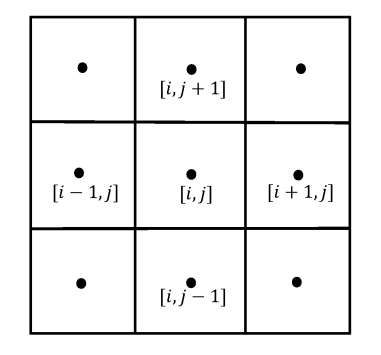
\includegraphics[width=0.8\linewidth]{img/intro/mStructured.png}
    \caption{}
    \label{fig-structured-ij}
  \end{subfigure}%
  \begin{subfigure}{0.5\linewidth}
    \centering
    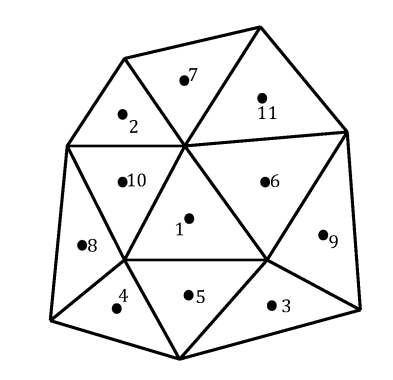
\includegraphics[width=0.8\linewidth]{img/intro/mUnstructured.png}
    \caption{fig-unstructured-ij}
    \label{fig-unstructured}
  \end{subfigure}%
  \caption{}
  \label{fig-structured-unstructured}
\end{figure}

\section{Structured and Unstructured Meshes}

The evolution of mesh generation can be correlated to the evolution of compute power available to the boffins. With the advent of third generation computers (1964-1971) carryinig integrated circuits, engineers were able to automate some of the manual processes in mesh generation. Meshes consisting of a template that repeats itself could be generated. These meshes were called \textit{structured meshes} as their adjacencies or relationships could be known implicitly. Consider a grid in two dimensions as shown in Figure \ref{fig-structured-ij}. Given a cell $(i,j)$ we can identify its neighbours as $(i-1, j)$ to the left and $(i+1, j)$ to the right. Similarly, cell $(i, j+1)$ will be to the top and $(i, j-1)$ would be to its bottom. The connectivity pattern repeats in such a mesh. Figure \ref{fig-structuredNaca0012} shows a structured mesh generated for NACA 0012 airfoil around its leading edge. Notice the implicit connectivity of the cells even though the size of mesh elements is varying.

\begin{figure}
  \centering
  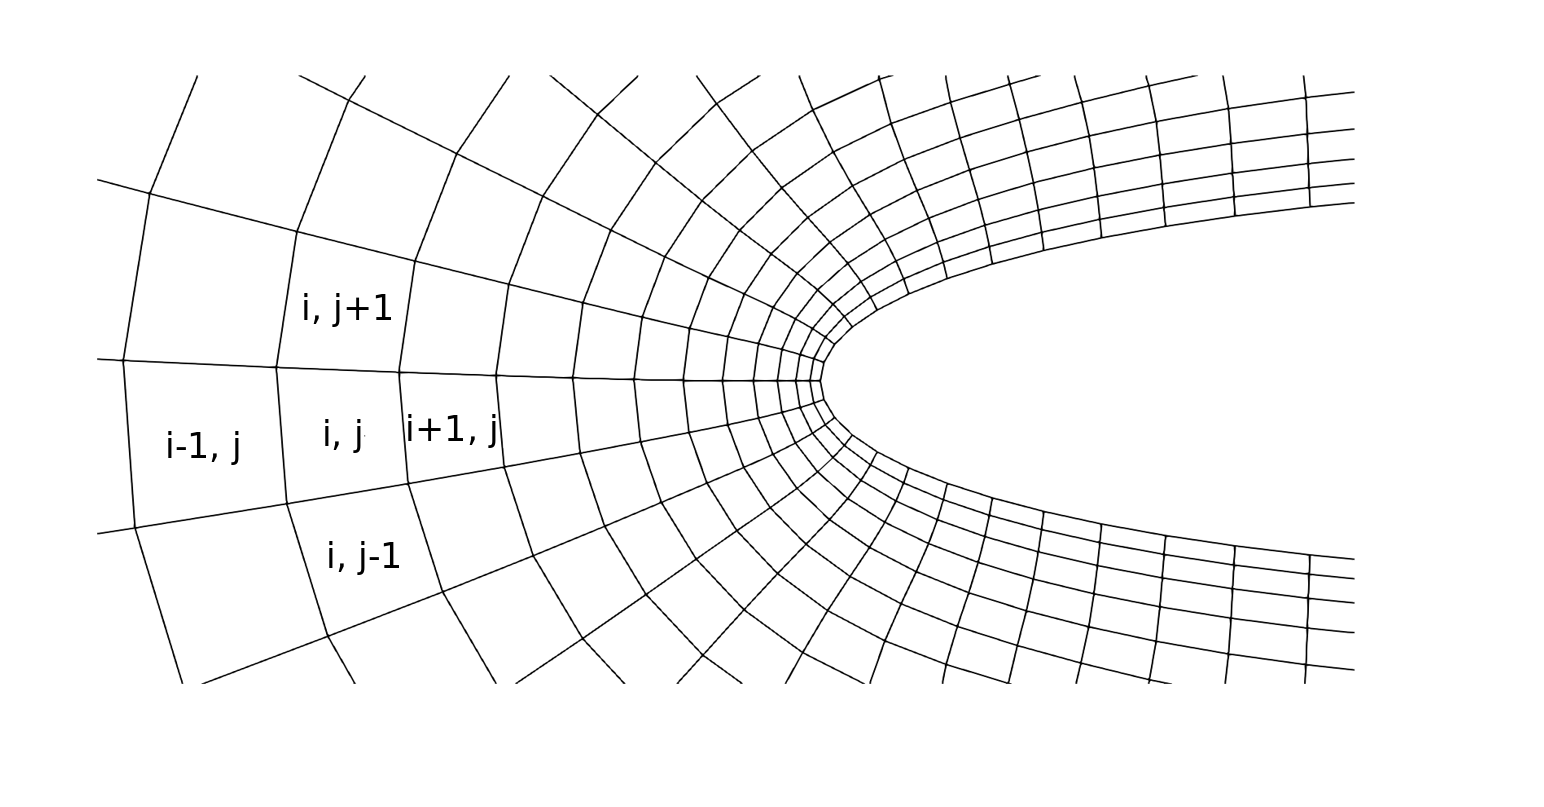
\includegraphics[width=0.8\linewidth]{img/intro/stucturedNaca0012.png}
  \caption{Structured mesh around leading edge of a NACA 0012 airfoil}
  \label{fig-structuredNaca0012}
\end{figure}


Structured meshes were attractive to engineers because of their low memory usage as the topology of the cells is repeated. Also, given simple domains to mesh, these meshes were optimal for minimizing the errors in CFD, resulting in faster simulations \cite{d1991optimal}. Programming CFD solvers with these meshes was easy as cell connectivity occurs in a regular fashion. However, as the scope of CFD simulations grew over time and more complex geometries were becoming commonplace, the task of generating structured meshes around them proved to be a daunting one. 

The disadvantage of using a structured mesh for more complex geometries is the increase in grid non-orthogonality or skewness that can cause unphysical solutions due to the transformation of the governing equations \cite{TU2013219}. The transformed equations that accommodate the non-orthogonality act as the link between the structured coordinate system (such as Cartesian coordinates) and the body-fitted coordinate system, but contain additional terms, thereby augmenting the cost of numerical calculations and difficulties in programming. Hence, a structured mesh may affect the accuracy and the efficiency of the numerical schemes used by a solver. Additionally, the tedious process of generating such meshes for more complex geometries was hard to justify. Hence, more flexible and automatic methods were devised. These methods produced meshes in a more random manner but with lesser human intervention. Broadly, the meshes produced by such methods were classified as \textit{unstructured meshes}. Figure \ref{fig-unstructured} shows an unstructured mesh. The arrangement of the mesh elements is random. Along with the shape of the elements, we need a data structure to store the adjacencies of the mesh.

The cost of finding flux at a wall, a widely used parameter in Finite Volume Methods (FVM) for fluid flow simulations, for unstructured meshes is high as compared to their structured counterparts. Also, the amount of memory usage is also high as the topology of the mesh is no longer repeated. Still, they are more widely used today because of their capability to handle arbitrary complex geometries, their capability to automate the mesh generation process and their flexibility in refinement based on the geometry topology and/or the solution gradients. Figure \ref{fig-unstructuredNaca0012} shows an unstructured mesh at the leading edge of a NACA 0012 airfoil. Notice the random arrangement of triangles around the airfoil geometry. The connectivity at each vertex of the mesh needs to be stored separately.

\begin{figure}
  \centering
  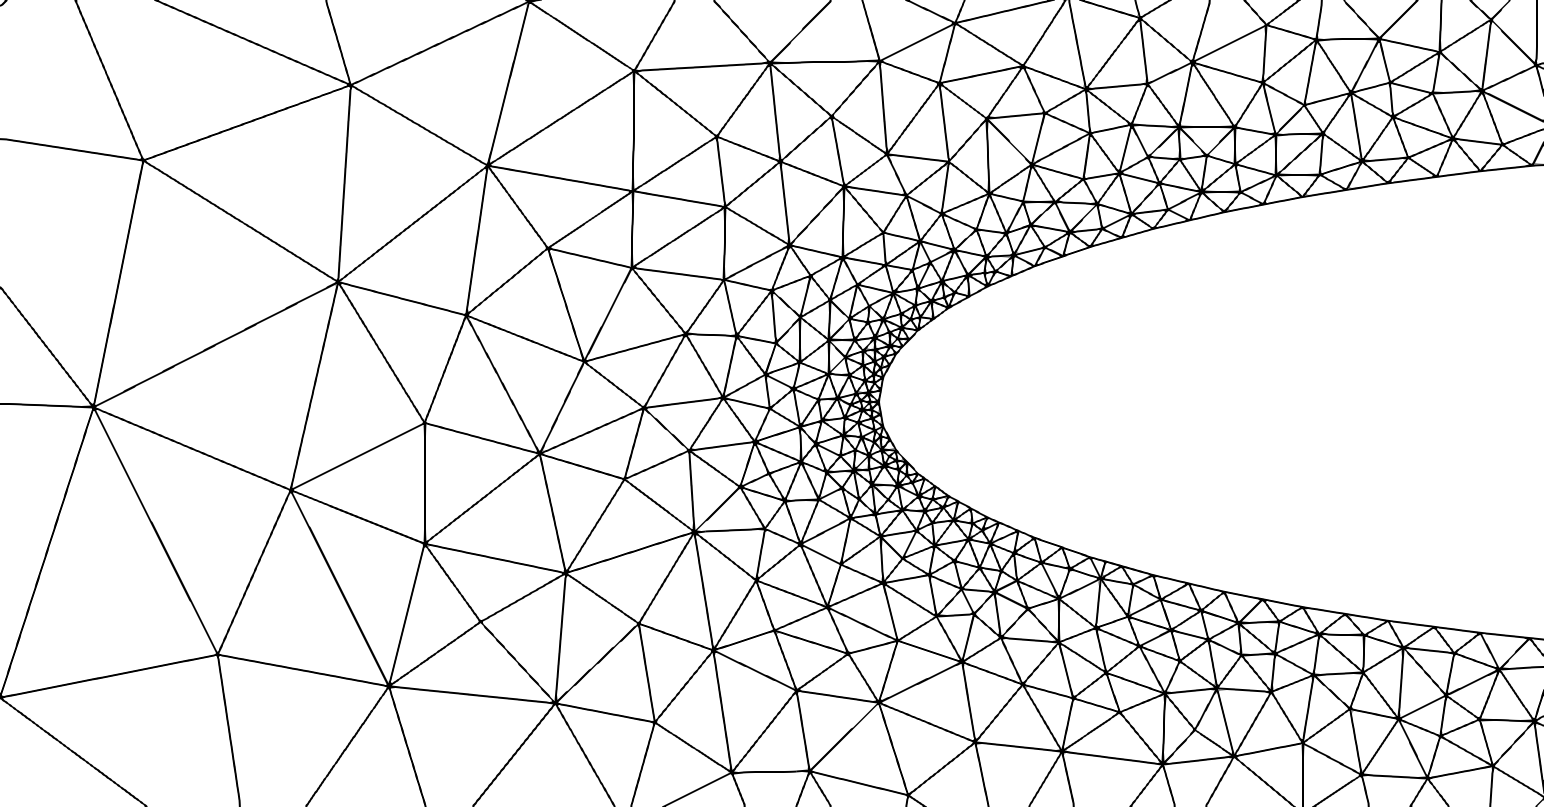
\includegraphics[width=0.8\linewidth]{img/intro/unstructuredNaca0012.png}
  \caption{Unstructured mesh around leading edge of NACA 0012 airfoil}
  \label{fig-unstructuredNaca0012}
\end{figure}

\section{Simplicial and Non-Simplicial Meshes}
\label{sec-simplicial}

Before discussing about simplicial and non-simplicial meshes, we need to define certain terms. In geometry, a simplex is a generalization of the notion of a triangle or tetrahedron to arbitrary dimensions. For example, a 0-simplex is a point, a 1-simplex is a line segment, a 2-simplex is a triangle and a 3- simplex is a tetrahedron. See Figure \ref{fig-simplices} for an illustration.

\begin{definition}
A \textbf{k-simplex} is a k-dimensional polytope which is the convex hull of its k+1 vertices
\end{definition}

A simplicial complex is a set composed of points, line segments, triangles, and their n-dimensional counterparts. In other words, a simplicial complex is a set strictly containing simplices only. Figure \ref{fig-simplicialComplex} shows a three-dimensional simplicial complex.

\begin{definition}
A \textbf{simplicial complex} K
is a set of simplices that
satisfies the two following
conditions:
a) Any face of a simplex
 from K is also in K
b) The intersection of any
 two simplices S1 and S2
 is either $\phi$ (null set) or a face of
 both S1 and S2
\end{definition}

\begin{figure}
	\centering
	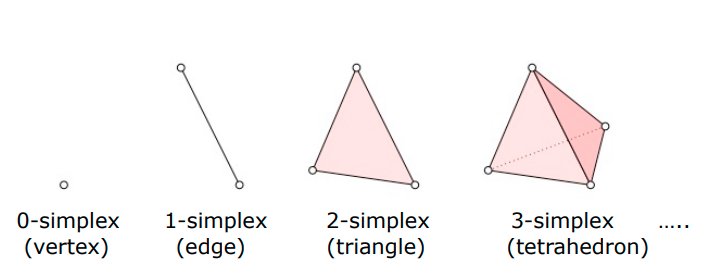
\includegraphics[width=0.95\linewidth]{img/intro/simplices.png}
	\caption{$n$ dimesnional simplices.}
	\label{fig-simplices}
\end{figure}

A mesh which contains only simplicial mesh elements is called a simplicial mesh. For example, a mesh which contains only triangular simplices is called a triangulaiton. In other words, a \textbf{triangulation} is the division of a surface or plane polygon into a set of triangles, usually with the restriction that each triangle side is entirely shared by two adjacent triangles. It was proved in 1925 that every surface has a triangulation, but it might require an infinite number of triangles. Figure \ref{fig-triangulation} shows a triangulation of a torus.

\begin{definition}
	A \textbf{triangulation} of a topological space X is a simplicial complex K, homeomorphic to X, together with a homeomorphism h: K $\rightarrow$ X.
\end{definition}

A non-simplicial mesh is simply a mesh which is not simplicial. Such a mesh contains mesh elements other than simplices too. For example, in two dimensions, a mesh which contains quadrilateral elements or quads will be called a non-simplicial mesh. In three dimensions, a mesh containing hexahedral elements would fall under the category of non-simplicial meshes.

Simplicial elements have been traditionally used for mesh generation. These elements are simple to work with and provide good flexibility in terms of discretization of a domain. These benefits make simplicial meshes very simple to produce. However, some of the drawbacks of simplicial meshes have led to mesh generation techniques with non-simplicial elements. Consider a triangulation of a surface. The Euler Formula states that for any convex polyhedron, the number of vertices and faces together is exactly two more than the number of edges. Mathematically,

\begin{equation}
V-E+F=2
\label{eqn-eulerFormula}
\end{equation}

where $V$ is the number of vertices, $E$ is the number of edges and $F$ is the number of faces in the polyhedron. For a triangulation, each edge is shared by two faces. Also, each face has three edges associated with it. Hence, the number of faces is $2/3$ times the number of edges, or $F= (2/3) \times E$. Substituting this in equation \ref{eqn-eulerFormula}, we get

\begin{align}
\begin{split}
		V - E + F  & = 2 \\
		V - E + \frac{2}{3} \: E & = 2 \\
		V - \frac{1}{3} \: E & = 2 \\
		3V & \approx E
		\end{split}
\end{align}

Hence, the number of edges is three times the number of vertices in a triangulation (asymptotically). On the other hand, the number of edges is two times the number of vertices for a closed quadrilateral surface mesh. A similar derivation could be done for three-dimensional simplicial and non-simplicial elements. The number of edges in a tetrahedral mesh is about seven times the number of vertices. On the other hand, in a hexahedral mesh, the number of edges is only about three times the number of vertices (asymptotically). Higher connectivity for simplical meshes leads to higher computational cost when refining the mesh using a vertex-based discretization methods. Hence, non-simplicial meshes are substantially more efficient than simplical meshes for a given number of unknowns or grid points.

\begin{figure*}
\begin{minipage}{0.45\linewidth}
	\centering
	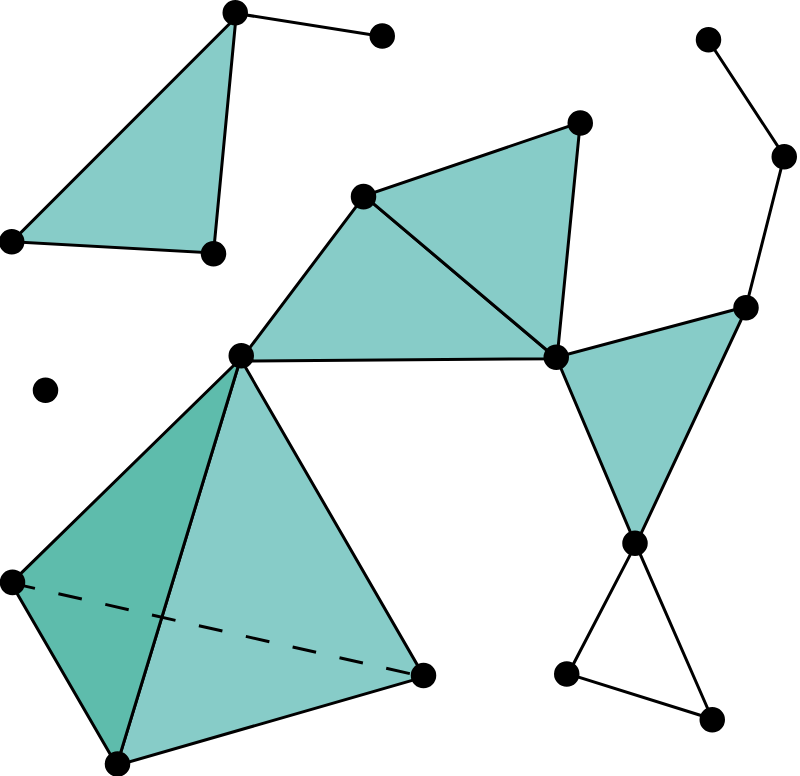
\includegraphics[width=\linewidth]{img/intro/simplicalComplex.png}
	\caption{A three-dimensional simplicial complex.}
	\label{fig-simplicialComplex}
\end{minipage}\hfill
\begin{minipage}{0.45\linewidth}
	\centering
	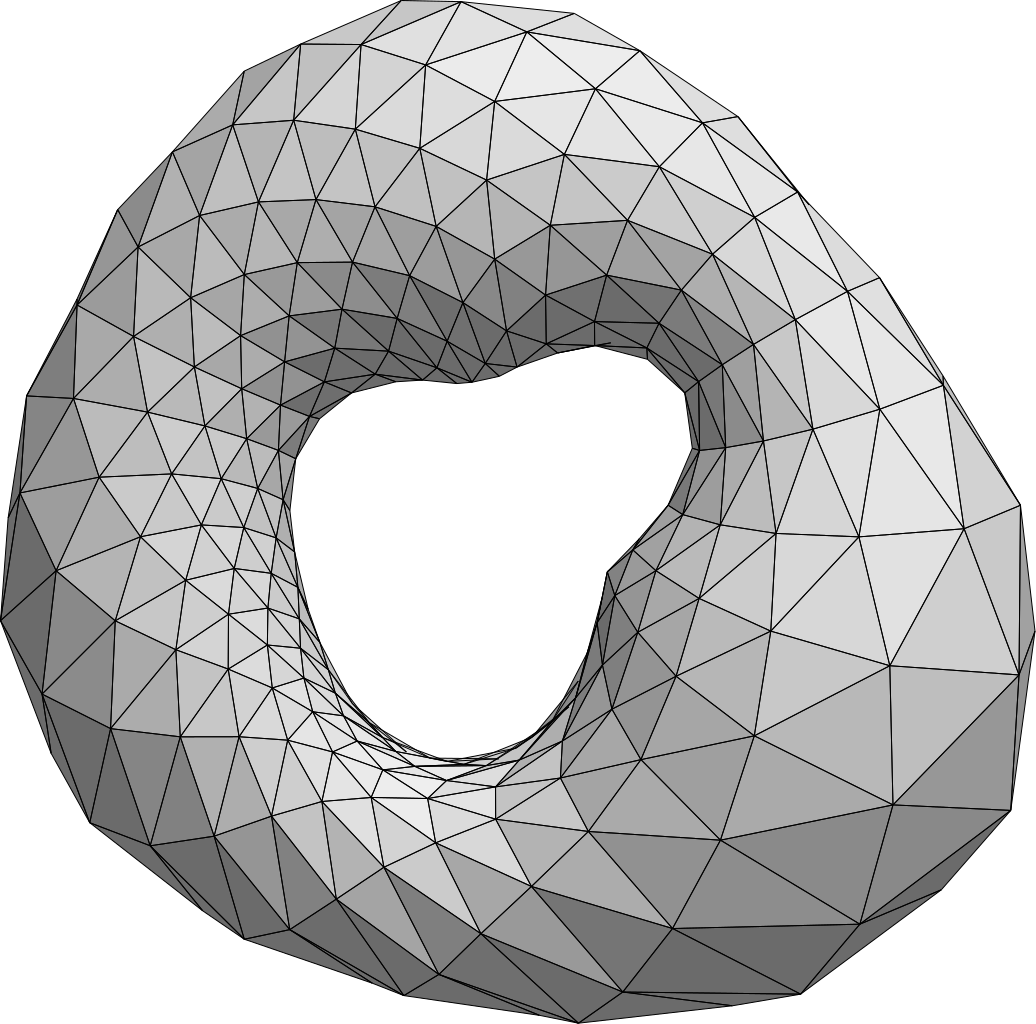
\includegraphics[width=\linewidth]{img/intro/triangulation.png}
	\caption{Triangulation of a torus.}
	\label{fig-triangulation}
\end{minipage}
\end{figure*}

Additionally, regular arrays of nonsimplical elements may also enhance accuracy, owing to a local cancellation of truncation errors that may not occur on groups of nonsimilar simplical elements \cite{mavriplis1997unstructured}. In two-dimensions, quadrilateral elements have been preferred over triangles in highly stretched two-dimensional grids due to their lower connectivity \cite{aftosmis1994accuracy}. These advantages of non-simplical mesh elements have resulted in fully non-simplicial mesh generation techniques \cite{blacker1991paving, zhu1991new}. The scheme introduced by Blacker \etal \cite{blacker1991paving} uses a paving methodology with several mesh element collision checks and special conditions for the concave corners to generated an isotropic all-quad two-dimensional mesh for complex geometries. One such mesh is shown in Figure \ref{fig-quadMesh}.

\begin{figure}
	\centering
	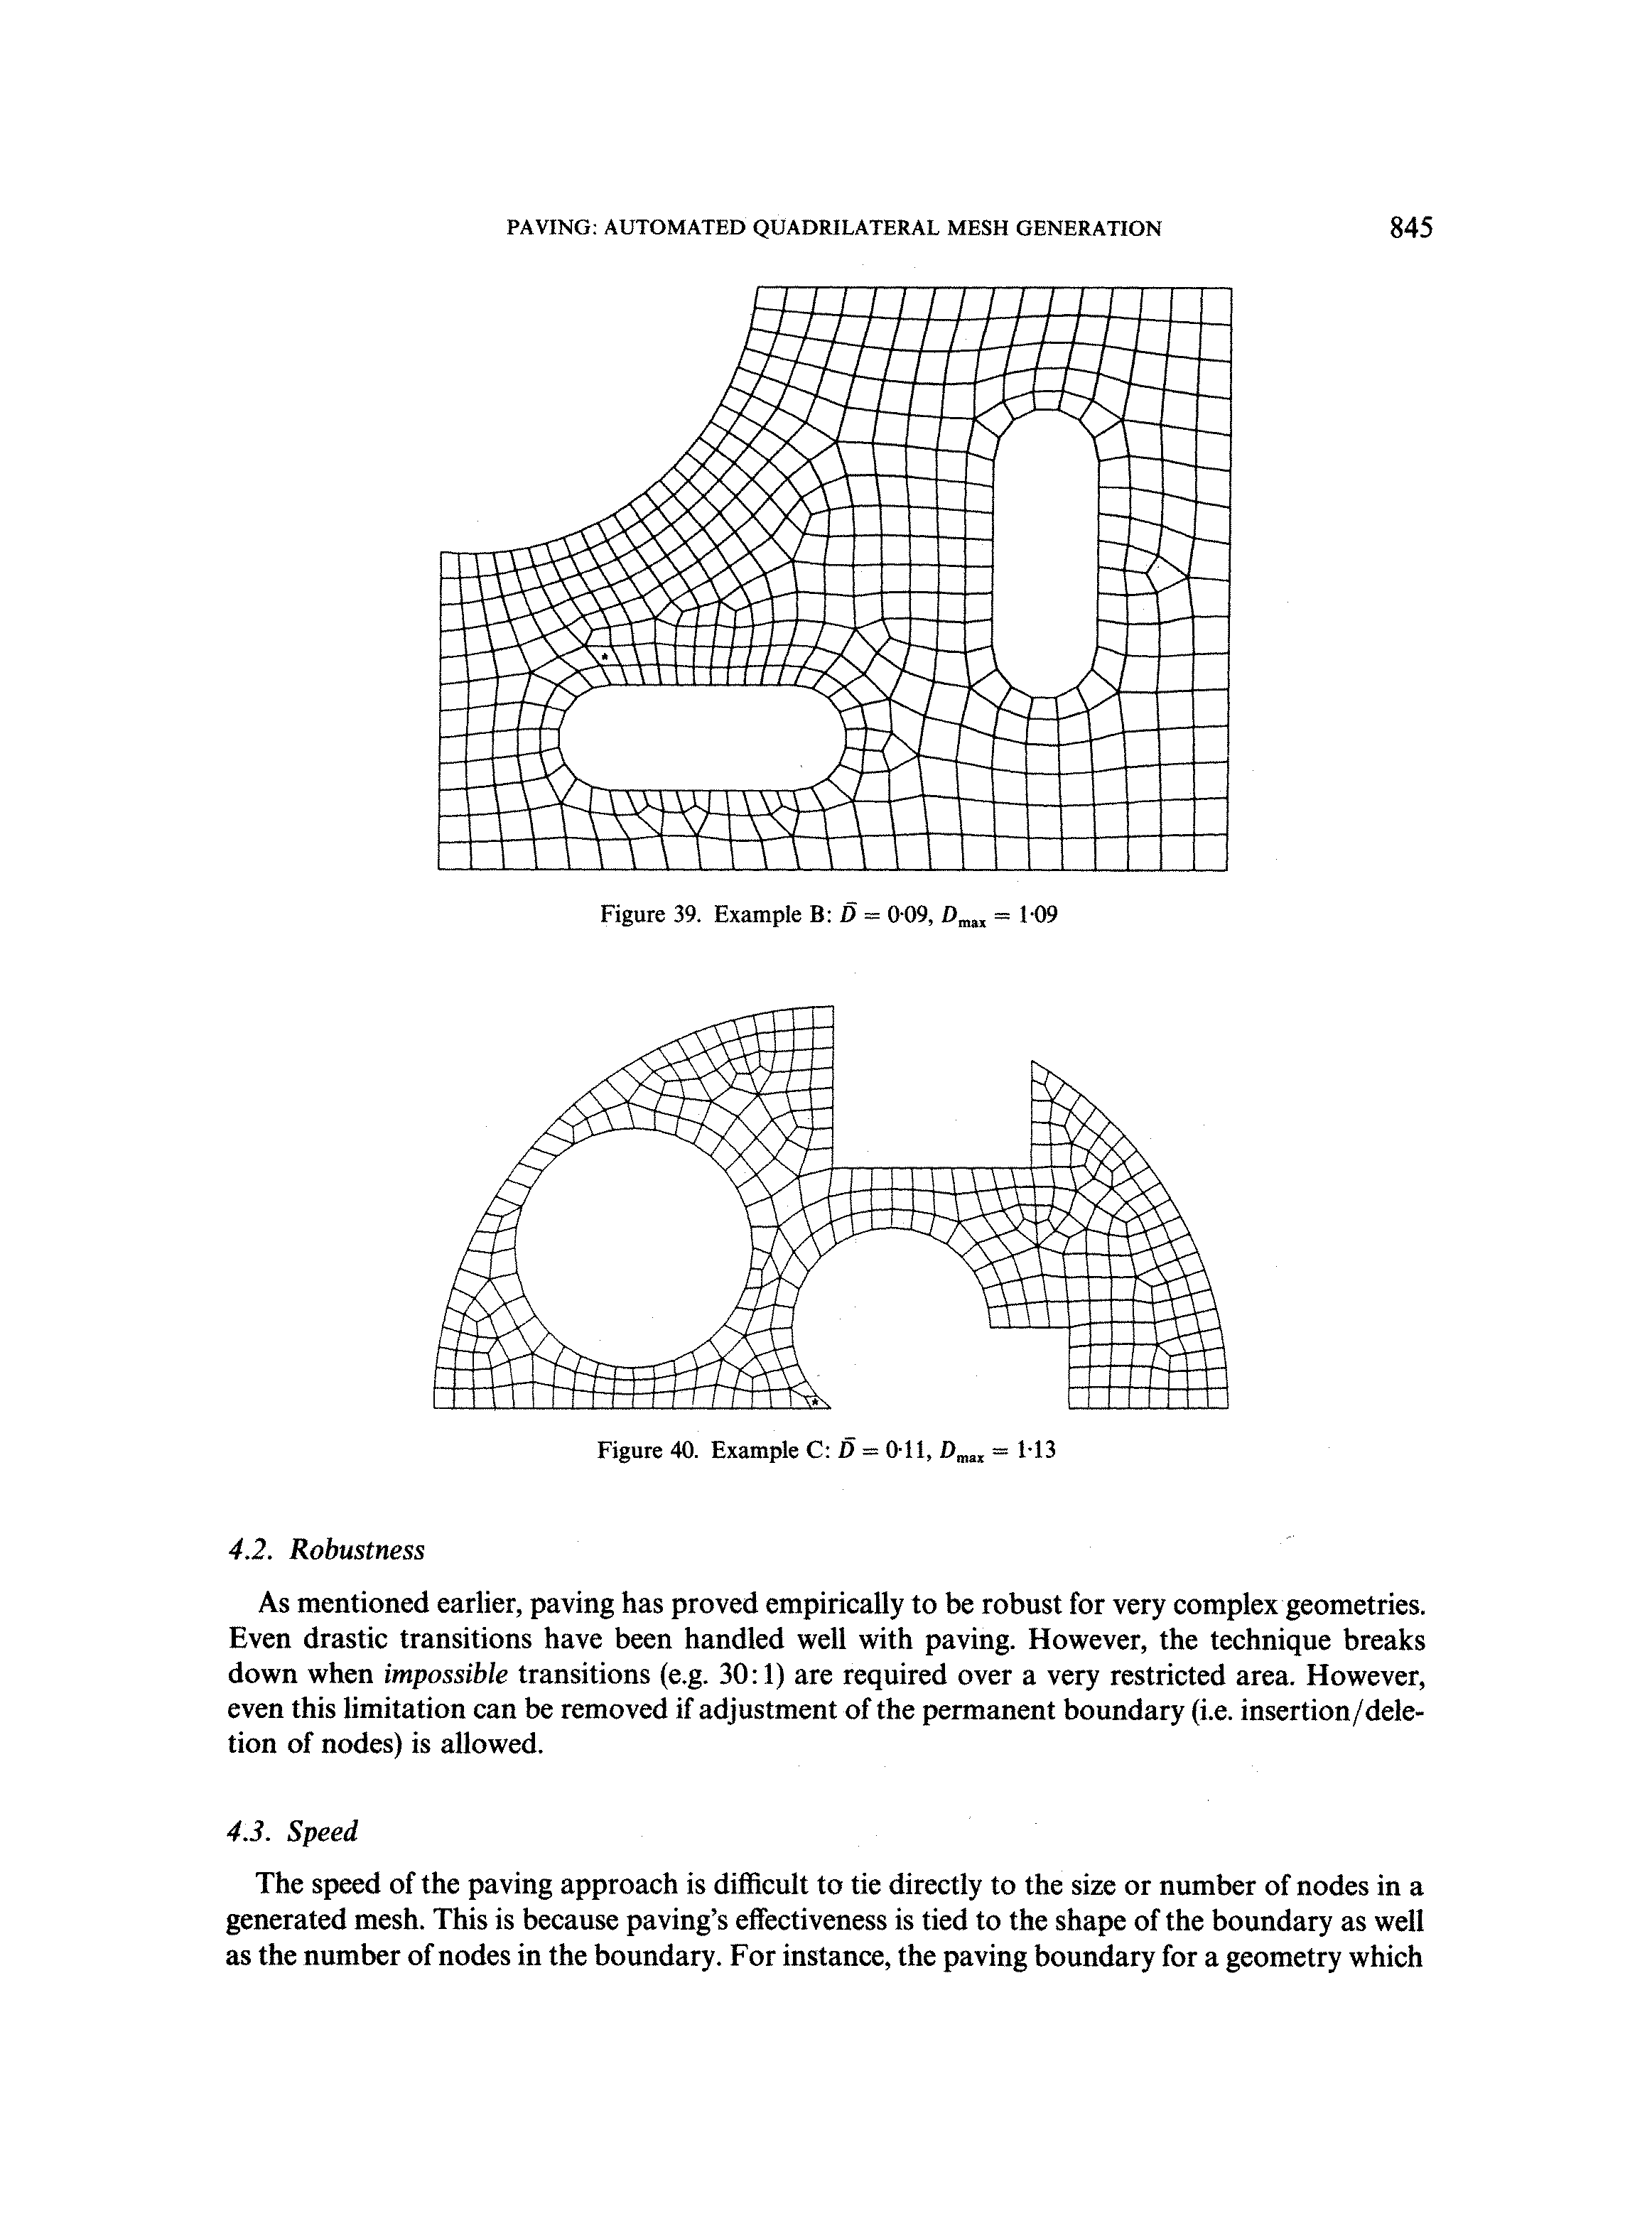
\includegraphics[trim={0 65.5cm 0 14cm },clip,width=\linewidth]{img/intro/lit/quadMesh.png}
	\caption{A non-simplical quad mesh generated with paving methodology \cite{blacker1991paving}.}
	\label{fig-quadMesh}
\end{figure}

Even though non-simplical mesh elements have been favored for a variety of scenrarios in mesh generation, and especially while generating highly-stretched elements, they have their cons. It is significantly difficult to generate an automatic mesh generation strategy which creates non-simplicial mesh conforming to complex surface and 3D geometrical configurations. Manual input is usually required to mesh such geometries. In these situations, simplical mesh elements are quite useful in dealing with the complexity in the geometry. Hence, a hybrid mesh containing both simplical and non-simplical mesh elements is a reasonable choice for mesh generation. We would revisit this in section \ref{sec-motivation} where we reason about choosing a hybrid scheme to mesh the surface.

\section{Boundary Layer Meshes}
\label{sec-boundaryLayerMesh}

With the advent of several unstructured mesh generation techniques, a broader selection of geometries could be dealt with. This immensely increased the scope of CFD solvers and pushed the limits of numerical methods in terms of accuracy and speed. However, a different approach was needed for the parts of the mesh in which viscous forces were more dominant as compared to the inertial forces. In other words, at the location of the viscous boundary layer, the gradient of physical measures like velocity is several magnitudes higher in one direction as compared to its orthogonal direction. A mesh generation technique which would help in resolving such strong gradients of the velocity in the boundary layer was required. For example, consider a flow over a flat plate as shown in Figure \ref{fig-boundaryLayer}. The velocity of the fluid at the surface of the plate is zero. However, the velocity becomes freestream velocity $u_0$ very near to the surface. The thickness of this layer of fluid, where the velocity of the fluid goes from a value of zero to a value of around 0.95 times the freestream velocity is called the boundary layer thickness $\delta$. It is also called the viscous boundary layer as the viscous effects are dominant in this region of the flow.

\begin{figure}
  \centering	
  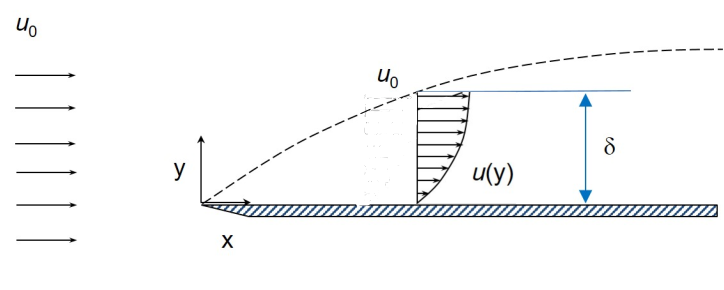
\includegraphics[width=0.8\linewidth]{img/intro/boundaryLayer.jpg}
  \caption{Fluid flow over a flat plate.}
  \label{fig-boundaryLayer}
\end{figure}

\section{Anisotropic Meshing}

The need to resolve the steep gradients at the boundary layer of the fluid flow gave rise to a type of mesh development strategy called anisotropic meshing. An anisotropic mesh is simply a mesh which has highly stretched elements. In other words, the aspect ratio of the elements for an anisotropic mesh would be really high. Aspect ratio of a mesh element is simply a size measure of the element. For tris and quads, the ratio of the length of the largest edge of the element to the smallest one is usually taken as the aspect ratio of that element. Figure \ref{fig-AR} illustrates some different aspect ratio triangular and quadrilateral elements. 

To attain a highly anisotropic packing of the cell elements, it is required to provide large number of Degree Of Freedoms (DOFs) along the direction of steep gradients of physical quantities such as velocity. Traditionally generated isotropic meshes are incapable of resolving such steep gradients \cite{frey2005anisotropic}. 

\begin{figure}
	\centering
	\begin{subfigure}{0.5\linewidth}
	  \centering
	  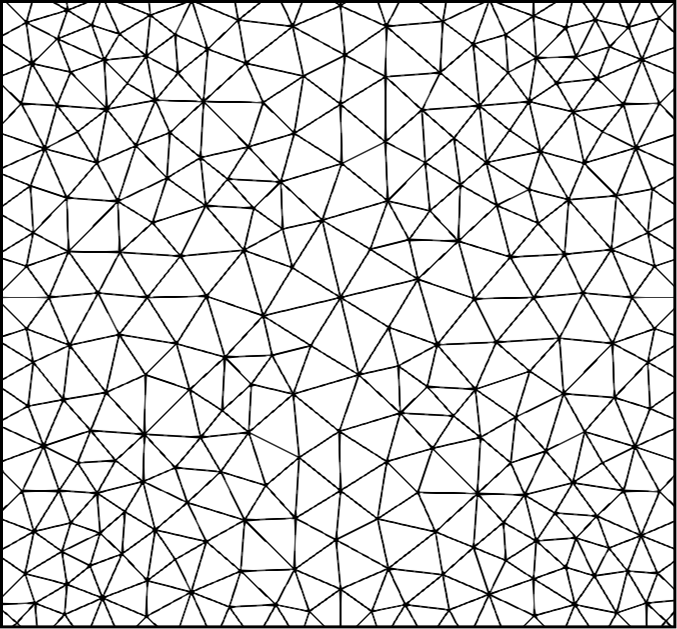
\includegraphics[width=0.9\linewidth]{img/intro/isotropic.png}
	  \caption{Isotropic mesh}
	  \label{fig-isotropic}
	\end{subfigure}%
	\begin{subfigure}{0.5\linewidth}
		\centering
		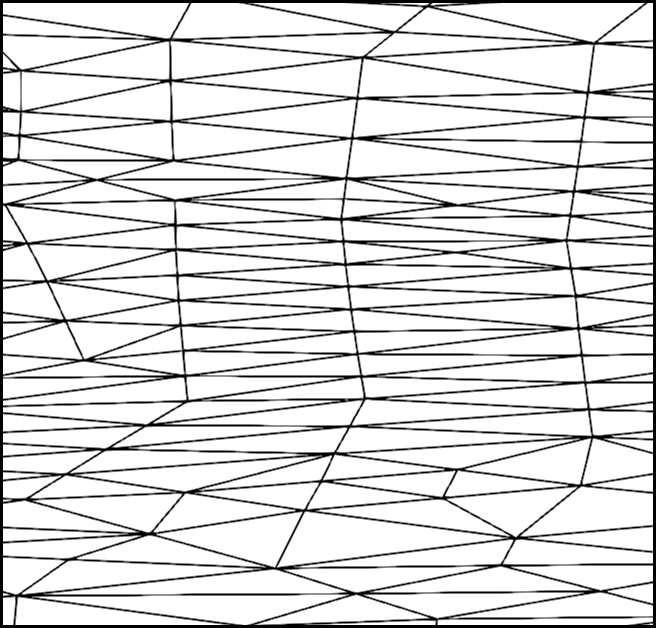
\includegraphics[width=0.88\linewidth]{img/intro/anisotropic.png}
		\caption{Anisotropic Mesh}
		\label{fig-anisotropic}
	\end{subfigure}
	\caption{Isotropic and Anisotropic Mesh Fragments}
	\label{fig-isotropic-anisotropic}
\end{figure}

Figure \ref{fig-isotropic} shows an isotropic mesh. The mesh elements have almost equal edge lengths. Here, the mesh elements are triangles and resemble equilateral triangles for most parts of the mesh. Given a point in the mesh, all the directions are the same and there isn't any bias towards a particular direction. For an isotropic physical process, such a mesh will serve the purpose and resolve gradients in all directions given the resolution of the mesh is appropriately chosen. However, if the physical process to be simulated is highly anisotropic, such as the velocity distribution along the boundary layer of the flat plate, as discussed in section \ref{sec-boundaryLayerMesh}, such a mesh will fail to resolve the steep velocity gradients. It would have to be refined to get the required refinement at the boundary, increasing the total number of DOFs in the mesh by a polynomial factor. Hence, a more reasonable mesh generation strategy is needed.

Figure \ref{fig-anisotropic} shows an anisotropic mesh. The triangular elements of the mesh are highly streched, with one edge being considerably shorter than the other two. The number of DOFs is distributed over the domain in a fashion so as to have the majority of the DOFs along the steep gradients of the physical quantities to be simulated. Hence, cell alignment with the solution to capture anisotropic flow features is possible with such a mesh.

\begin{figure}
	\centering
	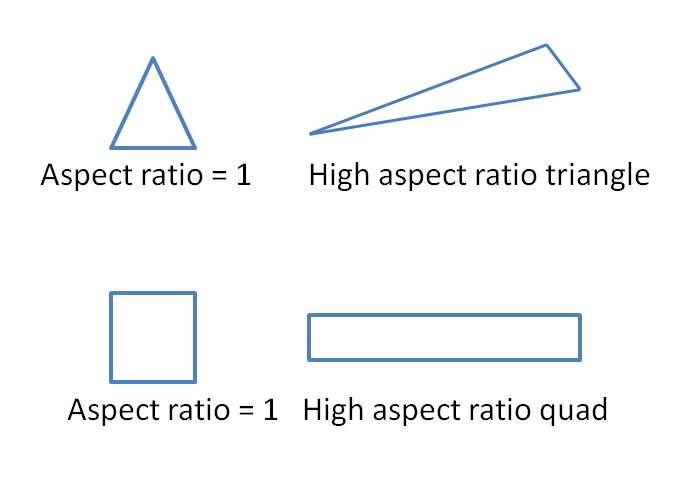
\includegraphics[width=0.6\linewidth]{img/intro/aspectRatio.png}
	\caption{Illustration of different aspect ratio triangular and quadrilateral elements.}
	\label{fig-AR}
\end{figure}

\subsection{Brief Literature Review - Anisotropic Meshing}

Several techniques have been developed to generate meshes in two dimensions with some sort of anisotropy. Some of these techniques have also been generalized to surfaces. However, isotropically-meshed surfaces with a smooth element-size variation are generally easier to mesh than anisotropically-meshed surfaces with strong size variations \cite{TU2013219}. Many techniques developed in 2D have been generalized to 3D while some new methodologies have been deviced for volume meshing. We go over some of these methods briefly.

\subsubsection{2D and Surfaces}

Most of the initial attempts at generating stretched element meshes in two dimensions used a Delaunay mesh and a locally mapped space to get the required level of anisotropy  \cite{mavriplis1990adaptive}. A mesh generated by such a method is shown in Figure \ref{fig-mavri}. Some techniques used an approach of using a locally structured or semi structured mesh for the regions requiring high anisotropy  \cite{nakahashi1987fdm}.

\begin{figure*}
\centering
\begin{minipage}[b]{.4\textwidth}
	\centering
	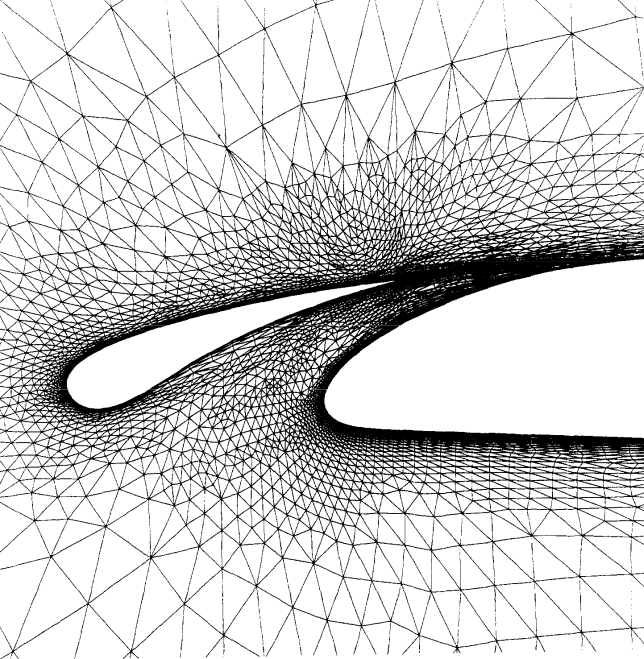
\includegraphics[width=\linewidth]{img/intro/lit/mavri.png}
	\caption{Illustration of adaptively refined mesh for the two-element airfoil configuration near the gap region \cite{mavriplis1990adaptive}.}
	\label{fig-mavri}
\end{minipage}\hfill
\begin{minipage}[b]{.55\textwidth}
	\centering
	\begin{subfigure}{\linewidth}
	\centering
	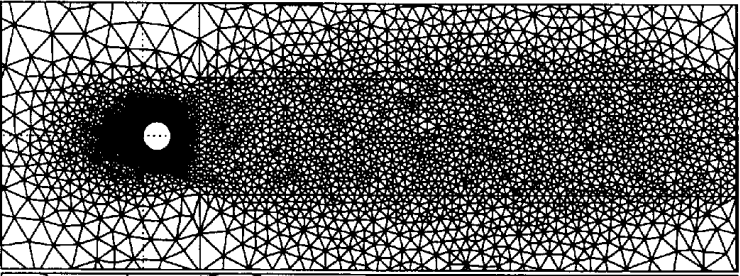
\includegraphics[width=\linewidth]{img/intro/lit/castroInitial.png}
	\caption{}
	\label{fig-castroInitial}
	\end{subfigure}
	\begin{subfigure}{\linewidth}
		\centering
		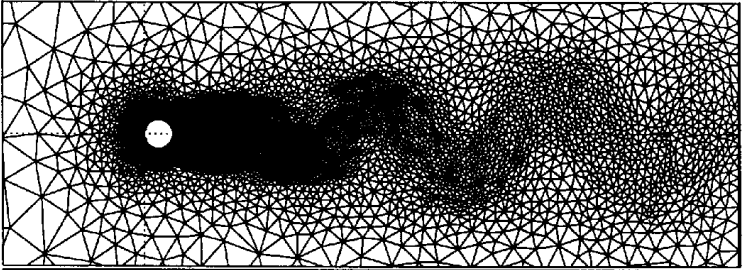
\includegraphics[width=\linewidth]{img/intro/lit/castro.png}
		\caption{}
	\label{fig-castro}
	\end{subfigure}
	\caption{Initial mesh (a) and adaptively generated anisotropic mesh (b) using solution metric evaluation	\cite{castro1997anisotropic}.}
\end{minipage}
\end{figure*}

Many attempts at generating anisotropic meshes come under the category of metric adaptation of the mesh. These techniques generally used a Delaunay type initial mesh and refined it anisotropically using a solution metric. Shimada \etal provided an automated method to obtain anisotropic triangulation of a parametric surface. Given a domain geometry and a tensor field that specifies desired anisotropic node-spacing, a proximity-based interacting force field is defined and the force balance configuration is dynamically simulated \cite{shimada1997anisotropic}. Castro \etal applied mesh adaptation technique to generate anisotropic meshes, to compressible viscous flows for a wide range of Reynolds and Mach numbers \cite{castro1997anisotropic}. An illustration of this method can be seen in Figure \ref{fig-castro}. 

Kunert \etal showed an anisotropic mesh generation algorithm that refines the mesh anisotropically by calculating the local error estimate on the initial mesh \cite{kunert2002toward}. This algorithm was presented for both two dimensional and three dimensional meshes. Another mesh adaptation technique by Li \etal tried to align the mesh to a calculated metric tensor from the physics of the problem \cite{li2010anisotropic}. Figure \ref{fig-anisotropicMeshAdaptation} shows one such mesh.

\begin{figure*}
\centering
\begin{minipage}[b]{.44\textwidth}
	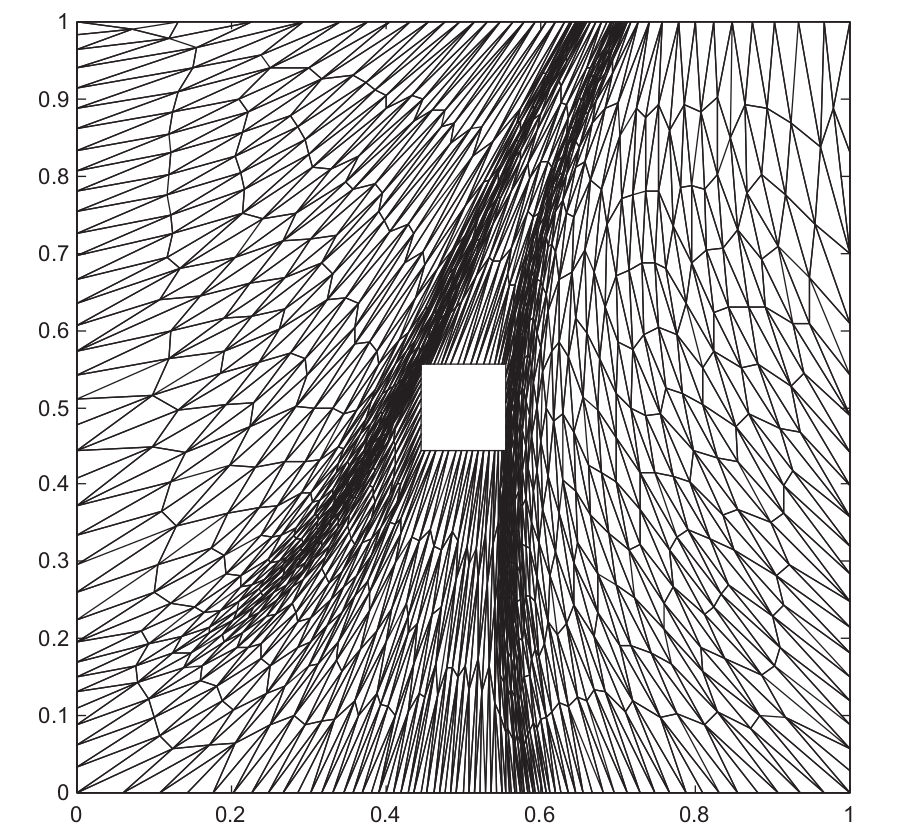
\includegraphics[width=\linewidth]{img/intro/lit/anisotropicMeshAdaptation.png}
	\caption{Anisotropic mesh generated by aligning the mesh elements to a metric calculated from an isotropic mesh solution \cite{li2010anisotropic}.}
	\label{fig-anisotropicMeshAdaptation}
\end{minipage}\hfill
\begin{minipage}[b]{.44\textwidth}
	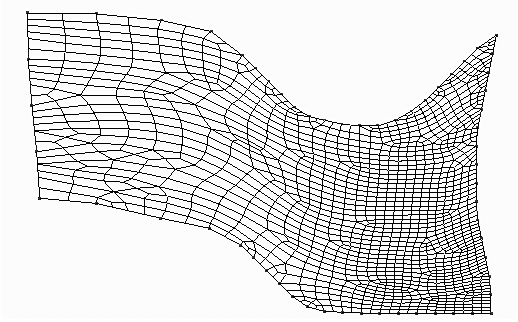
\includegraphics[width=\linewidth]{img/intro/lit/anisotropicQuadMesh.png}
	\caption{Anisotropic quadrilateral mesh generated with an input triangulation and solution contours \cite{viswanath2000quadrilateral}.}
	\label{fig-anisotropicQuadMesh}
\end{minipage}
\end{figure*}

A family of anisotropic mesh generation techniques fall under the Advancing Layer category. A method introduced by Pirzadeh produced unstructured triangular/tetrahedral grids with high-aspect-ratio cells using the advancing layer or the grid-marching strategy \cite{pirzadeh1994unstructured}. Another method which used the advancing layer strategy, with several mesh collision checks, was introduced by Lohner \cite{lohner1993matching}. Here, the mesh was produced by inflating the boundary curves in the direction of surface normals. Special care was taken while dealing with the concave corners of the mesh so as to avoid mesh element collisions.

\begin{figure}
	\centering
	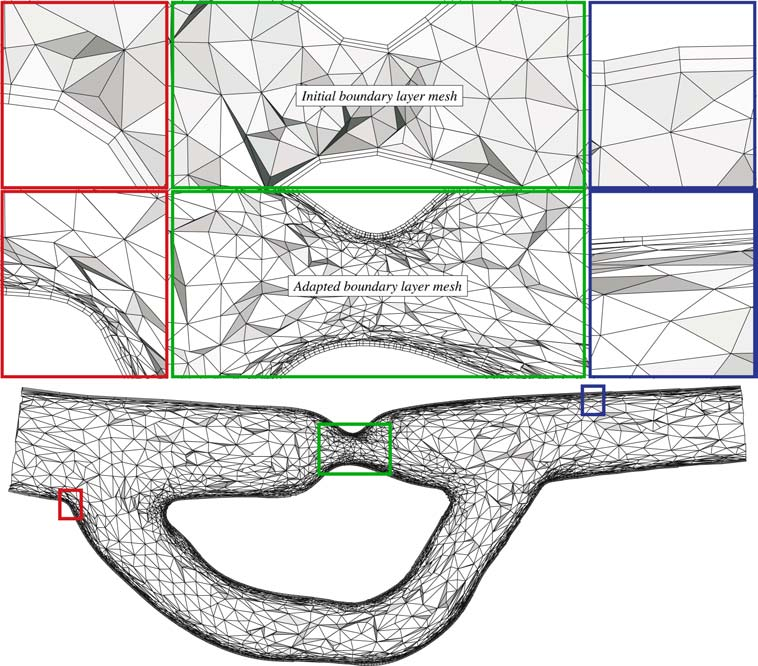
\includegraphics[width=0.8\linewidth]{img/intro/lit/sahni.png}
	\caption{ Collection of mesh faces cut by the vertical center- plane through the adapted boundary layer mesh of a porcine aorta. The windows correspond to magnified views which also show the initial boundary layer mesh \cite{sahni2008adaptive}.}
	\label{fig-sahni}
\end{figure}


While the majority of anisotropic mesh generation strategies focused on simplicial mesh elements, there have been some works which generate all quadrilateral (quad) surface meshes. A method by Lee \etal showed an anisotropic quadrilateral mesh generation scheme which generates a background triangular mesh and then proceeding with a cell merging procedure in the parametric space to produce the desired mesh \cite{lee2003new}. A different kind of method was adopted by Viswanath \etal to generate quadrilateral meshes with anisotropy and directional control \cite{viswanath2000quadrilateral}. A 2D geometric domain and desired level of anisotropy - as a metric tensor over the domain - specifying mesh sizing in two independent directions is taken as an input. Thereby node locations are calculated by closely packing recctangles in accordance with the inputs. An example mesh generated with this strategy is shown in Figure \ref{fig-anisotropicQuadMesh}.

\subsubsection{3D}
\label{sec-3D}

\begin{figure*}
\begin{minipage}{0.45\linewidth}
	\centering
	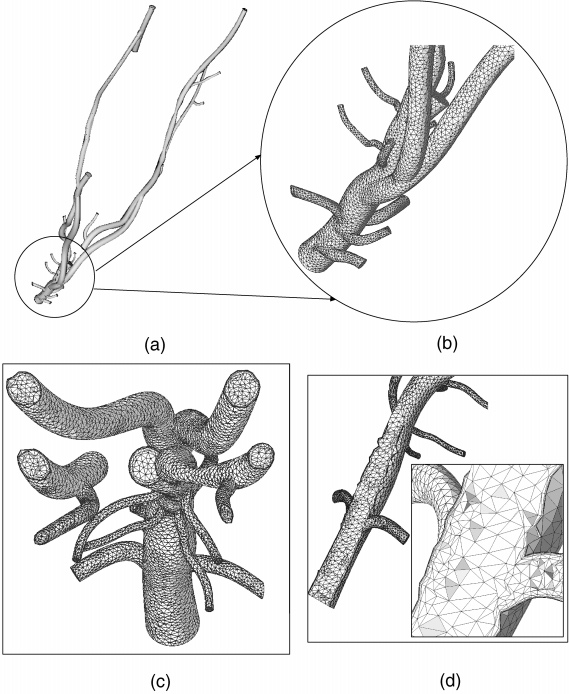
\includegraphics[width=\linewidth]{img/intro/lit/shephard.png}
	\caption{Boundary layer mesh for simulation of ow in blood vessels: (a) geometric model; (b) zoom in of surface mesh in the encircled region; (c);(d) cross-sections showing the boundary layer and isotropic meshes \cite{garimella2000boundary}.}
	\label{fig-shephard}
\end{minipage}\hfill
\begin{minipage}{0.45\linewidth}
	\centering
	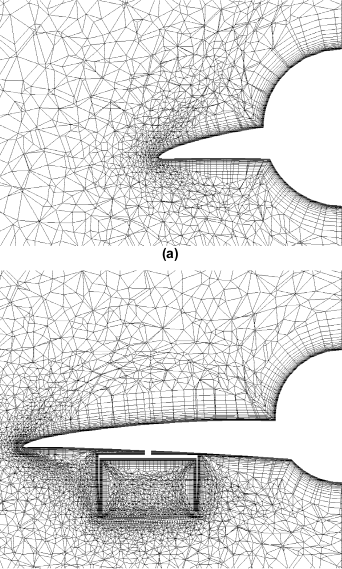
\includegraphics[width=\linewidth]{img/intro/lit/ito.png}
	\caption{Hybrid grid for an aircraft (NAXST-2). Two images show the cross-section of the mesh at three different locations along the chord of the airfoil \cite{ito2002unstructured}.}
	\label{fig-ito}
\end{minipage}
\end{figure*}

Given an initial surface discretization, several 3D mesh generation algorithms have been generated to create anisotropic volume meshes. Many methods which generate two-dimensional anisotropic  meshes can be extended to 3D \cite{lohner1993matching, nakahashi1987fdm,castro1997anisotropic}.

A generalized advancing layer method for generating 3D boundary layer mesh was presented by Garimella \etal \cite{garimella2000boundary}. Model boundaries grow into the domain to fill to generate the mesh in this method. An example mesh can be seen in Figure \ref{fig-shephard}. Another method was introduced by Ito \etal \cite{ito2002unstructured}. Here, a hybrid mesh was generated which comprised of tetrahedra, prisms and pyramids. First, the domain was filled with an isotropic tetrahedral mesh. Subsequently, the boundary walls were shifted inwards and the resulting gap between the tetrahedra and the walls was filled up with prismatic elements. Figure \ref{fig-ito} shows a mesh generated using such a strategy. This mesh generation strategy, of using a highly anisotropic semi-structured mesh near the boundaries of the domain (however, with no gradation over the boundary of the domain), and an isotropic mesh further away from domain boundaries is quite common in 3D meshing. Another example of such a strategy is shown in the work done by Sahni \etal \cite{sahni2008adaptive}. Here, mesh adaptation was applied to a hybrid mesh, with semi-structured stretched elements at the boundary and isotropic elements away from the boundary. Figure \ref{fig-sahni} shows a mesh generated by this method.

The method used by Shimada and Yamada in two dimensions has also been extended to three dimensions to generate anisotropic tetrahedral meshes. Given an arbitrary input anisotropy function, the algorithm generates high quality anisotropic tetrahedral mesh that conforms to the input geometry \cite{yamakawa2000high}. A mesh generated from this method can be seen in Figure \ref{fig-yamakawa}.

\begin{figure}
	\centering
	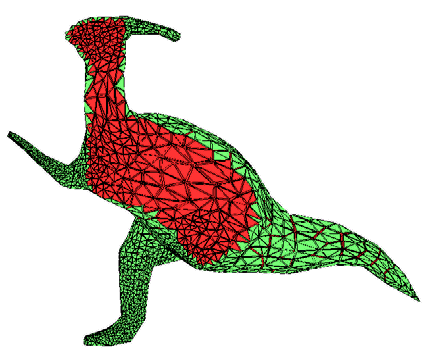
\includegraphics[width=0.5\linewidth]{img/intro/lit/highQualityTetMesh.png}
	\caption{Anisotropic Tetrahedral Mesh generated using ellipsoidal bubble packing methodology  \cite{yamakawa2000high}}
	\label{fig-yamakawa}
\end{figure}

In another work, a metric-orthogonal anisotropic mesh is generated. In addition to aligning the mesh to a metric, mesh elements are also aligned with the eigenvectors \cite{loseille20093d}. The quality of the input metric strongly affects the output mesh.

Another method which generates a hybrid mesh using semi-structured boundary layer mesh and an isotropic outer mesh was given by Ito \etal \cite{ito2007multiple}. Here, special treatment of sharp corners on the surface was done by adding multiple marching directions at the sharp corner. This resulted in generation of a better volume mesh. The research showed that if the corners of the surface mesh, from which the volume mesh is generated, are treated specially and are hence refined more than other regions of the surface, the volume mesh thus generated would be of superior quality. More importantly, such special treatments of sharp corners in the surface mesh helps to create semistructured elements (for viscous boundary layer mesh) around singular points on the surface. A very important problem addressed by this study is one of the pivotal reasons to write this thesis.

Consider Figure \ref{fig-cornerIto} from the work by Ito \etal \cite{ito2007multiple}. An intersection between three surfaces is considered. There are labeled $S_A, S_B$ and $S_C$. The surfaces can represent a wing upper surface, a blunt trailing edge and a fuselage, respectively. As most of the surface meshes are simplical, isotropic and don't treat corners specially, the task to generate a valid viscous boundary layer mesh from them is considerably difficult. This difficulty is compounded at complex corners like the one shown in the figure. The paper puts forward a technique to discretize the surface further by adding new nodes and faces to the surface at such corners. In the figure, nodes are added along the direction $BA$. This process helps in creating additional normal directions near the corners of the surface and solves the problem of singularity to a great extent.

\begin{figure}
	\centering
	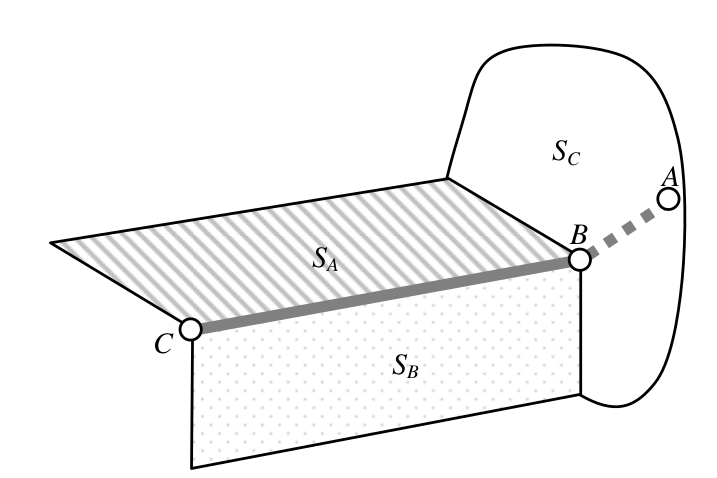
\includegraphics[width=0.8\linewidth]{img/intro/lit/cornerIto.png}
	\caption{Three boundary surfaces $S_A, S_B, $ and $S_C$ \cite{ito2007multiple}}
	\label{fig-cornerIto}
\end{figure}

\section{Motivation}
\label{sec-motivation}

\subsection{Surface Mesh Generation Strategies}

Stretched volume meshes are generated from an initial triangulation of a surface. These surfaces are usually represented by Non-Uniform Rational B-Splines or NURBS in various Computer Aided Design (CAD) packages. Generation of the surface mesh requires a separate methodology or algorithm as compared to the two-dimensional mesh generation as the mesh elements include a third dimension.

%%Method1

A majority of surface mesh generation methods produce a surface mesh from the parametric mapping of a two-dimensional mesh onto a surface \cite{george1998delaunay, chen1997delaunay}. Usually, a two-dimensional Delaunay mesh is generated over a parametric surface and then mapped onto the curved surface. This method is attractive as it is simple and there are a number of robust Delaunay mesh generation schemes available to generate the initial two-dimensional mesh. However, the mapping from 2D to 3D doesn't always give satisfactory results in terms of mesh element quality. Also, this method doesn't always form well shaped surface elements, especially when the surface derivatives vary over the domain \cite{owen1998survey}. Meshes generated by such methods are generally isotropic and simplical. Hence, in addition to dealing with the badly shaped elements, several other post-processing operations need to be applied to them before generating a boundary layer volume mesh.

%%Method2

A different approach to surface mesh generation is adopted by methods which use the first fundamental form of the surface. In such methods, a metric is derived from the parametric representation of the surface and mesh elements are placed over the surface in an advancing front fashion with respect to this metric. Culli\'ere deviced one such method where he used a nodal density function based on the curvature of the surface to discretize it \cite{cuilliere1998adaptive}. An advancing front triangular mesh generation method was presented where 3D parametric surfaces could be meshed with good quality mesh elements. Tristano \etal \cite{tristano1998advancing} presented a method which used a Riemannian surface definition to determine the amount of distortion of the elements in parametric space. Thereby, an advancing front method is applied to utilize this metric and generate good quality triangular elements over the surface. Figure \ref{fig-joseph} shows a mesh generated with this method. These methods, which use the parametric representation of the surface produce good quality triangular surface meshes. However, they are not well-suited to generate three dimensional anisotropic meshes with highly stretched elements. Additionally, the elements generated by such methods are simplical and hence, have their own drawbacks as discussed in section \ref{sec-simplicial}.

\begin{figure*}
	\centering
	\begin{minipage}{0.45\linewidth}
		\centering
		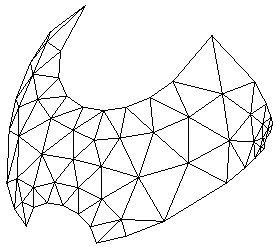
\includegraphics[width=\linewidth]{img/intro/lit/joseph.png}
		\caption{A CAD surface meshed with Reimannian space mesher}
		\label{fig-joseph}
	\end{minipage}
\end{figure*}

%%Method3

Lastly, surface meshes can also be generated by placing the mesh elements directly on the surface of the geometry. Lao and Lu \cite{lan1996finite} provide a method to produce a surface mesh over a given analytical surface. A given element density function is utilized and mesh elements are placed on the analytical surface using the advancing front technique. The elements are optimized considering factors such as surface curvature, element to element turning angle and the given density distribution, to get a high-quality surface mesh. Figure \ref{fig-lu} shows meshes generated with this method. With respect to being an input for a 3D viscous boundary layer mesh, these meshes have similar drawbacks as the ones discussed earlier. Mesh elements generated are triangular rather than quadrilateral or hybrid. Also, there is an additional input required to generate the mesh, which is the density function. Lastly, the boundary curves of the surface are not dealt with specially and the complete surface is isotropically meshed.

\begin{figure}
	\centering
	\begin{subfigure}{0.5\linewidth}
		\centering
		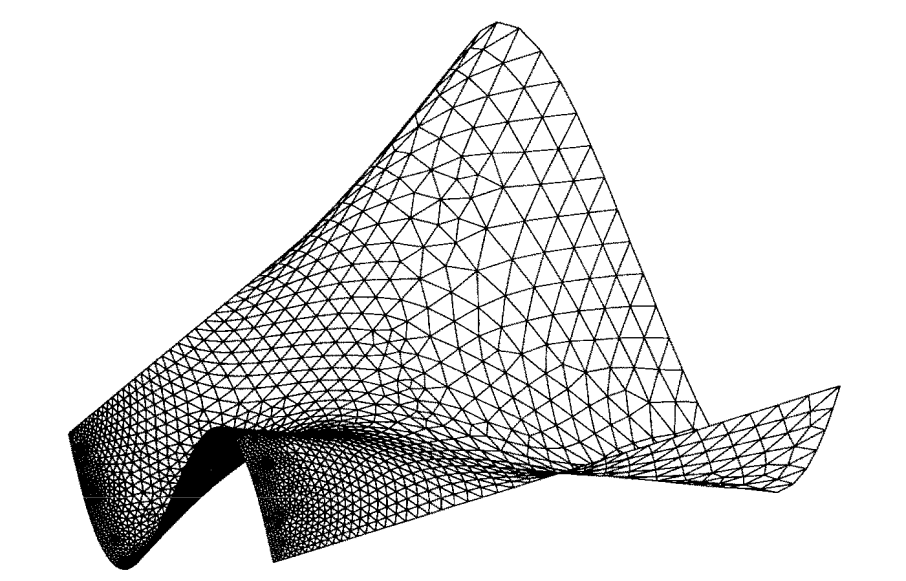
\includegraphics[width=\linewidth]{img/intro/lit/lu1.png}
		\caption{A ruled surface.}
		\label{fig-lu1}
	\end{subfigure}
	\begin{subfigure}{0.5\linewidth}
		\centering
		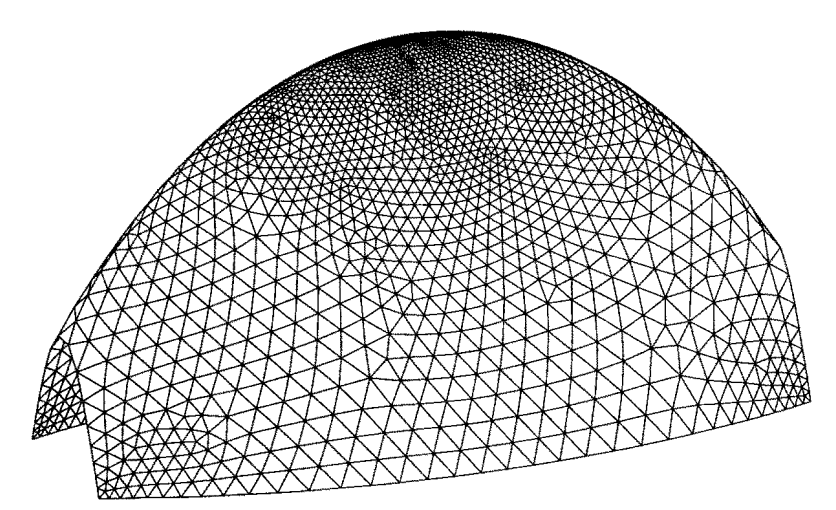
\includegraphics[width=\linewidth]{img/intro/lit/lu2.png}
		\caption{A free form surface.}
		\label{fig-lu2}
	\end{subfigure}
	\caption{Meshes generated directly over the surface by utilizing the analytical surface representation and element density distribution \cite{lan1996finite}.}
	\label{fig-lu}
\end{figure}

%%Consolidating

\subsection{Consolidating The Discussion}

%% 1. Hybrid
\subsubsection{Hybrid}
Consolidating our discussion on surface meshes, we find that most of the 3D surface meshes generated are triangular. In other words, these meshes are simplical. We discussed the pitfalls of using simplical mesh elements at the regions of anisotropy or at surface boundaries in \ref{sec-simplicial}. To recapitulate, higher vertex connectivity for simplicial meshes makes them inefficient when using a vertex-based discretization method. On the other hand, quad meshes in two dimensions and hex meshes in 3D are substantially more efficient than their simplicial counterparts for the same number of Degrees of Freedom. In addition to that, non-simplicial elements arranged in repeating arrays may enhance solution accuracy by local cancellation of truncation errors while their simplicial counterparts may fail to do so \cite{mavriplis1997unstructured}. Non-simplicial quadrilateral elements have been preferred over triangles in highly stretched two-dimensional grids due to their lower connectivity \cite{aftosmis1994accuracy}.

Even though non-simplicial elements are more efficient in mesh generation, conforming such elements to complex geoemtry remains a daunting task. Generally, manual input is required to generate all-quad surface meshes or all-hex volume meshes in the regions of geometric complexities. Hence, usage of simplicial mesh elements in these regions is a reasonable alternative. Hence, a surface mesh generation scheme is required, which generates a quad-dominant mesh with a very limited number of triangular elements. Regular arrays of highly-stretched quadrilateral elements should form the anisotropic boundary layer mesh. On the other hand, triangular elements could be used whenever one wants to conform to the geometry and increase the quality of the mesh elements generated.

%% 2. 3D
\subsubsection{Good Input For Anisotropic 3D Mesh}
Following the discussion from \ref{sec-3D}, it is particularly difficult to generate  hybrid 3D meshes from an isotropic surface discretization. At the minimum, several validation checks needs to be performed at the singularity points of the surface so as to generate a valid viscous 3D mesh. In addition to that, the anisotropy of the 3D mesh becomes extremely difficult to control at the complex corners of the surface if they are not handled specially. One solution discussed earlier was to add additional marching directions and nodes at the complex corners on the surface of the mesh so as to add additional normal directions near the complex corners. However, the root cause of the problem is the isotropic surface discretization which is completely unaware of its usage into a anisotropic 3D volume mesh generator. Hence, a better alternative is desirable which automates the process of special treatment of surface cusps.

%% 2. Automatic and Flexible
\subsubsection{Automatic and flexible}

The surface mesh generation methodologies either have several assumptions on the type of surfaces they can support or need a considerable amount of human intervention to complete. Specially for the cases where complex corners exist on the surface, a good surface mesh would need special arrangement of nodes and marching directions on the surface so as to produce a high-quality anisotropic volume mesh. Block structured meshes could be produced on a surface by manually discretizing the domain into several subdomains and meshing them using structured mesh generation technique independently. But again, the mesh generation process would be very tedious and would take a considerable amount of manpower. Hence, an automatic mesh generation technique which has a good level of anisotropy at surface boundary curves is desirable to serve as a good input to 3D mesh generation. Lastly, the mesh generation process could use flexibility in terms of the surface representation it can accept as an input. Many methods discussed earlier use the parametric form of the surface to generate the mesh. Additionally, some methods also require an element density distribution to be specified for the entire domain of the surface which needs to be meshed. These constraints again make it cumbersome to generate good quality surface meshes (for anisotropic volume meshes) for a wide variety of surface topologies. Hence, a method of surface mesh generation which accepts a more widely used surface representation is highly desirable.

\subsection{Advancing Layer Surface Mesh Generation}

We present a surface mesh generation algorithm that serves to address the aforementioned issues and carries desired qualities. The algorithm generates a surface mesh which has anisotropic characteristics normal to the boundary curves of the surface. The mesh elements are highly-stretched at these boundary curves of the surface and have a required level of directional anisotropy normal to the boundary curves. For the examples in this thesis, the boundary curves of the surface are chosen to be the curves where the surface normal direction jumps abruptly. Practically, the algorithm is independent of the selection of the boundary curves and can work for any selected set of boundary curves for a given surface. However, for the sake of automaticity and simplicity, the boundary curves are chosen to be the sharp features on the surface topology.

The surface discretization produced by the algorithm given in the thesis consists of a hybrid grid. Most of the elements (usually greater than 95\%) are quadrilateral mesh elements. Regular pattern of quad elements are repeated from the boundary curves of the surface towards its interior. This pattern helps retain the boundary curve topology towards the interior regions of the mesh. In addition to that, an appropriate discretization of the boundary curves of the surface can provide several additional normal directions to the surface near the boundary curves. This may be vital in solving the problem of complex corners or singularity points on the surface while generating a 3D viscous volume mesh.

With most of the elements on the mesh being non-simplicial, some triangular mesh elements are also utilized to discretize the surface. These elements are quite useful when dealing with complex surface topologies such as concave corners. Additionally, triangular mesh elements help to control the growth of the aspect ratio of the mesh elements as the mesh proceeds from the boundary towards surface interior. Overall, the surface mesh hence generated utilizes the advantages of both simplicial and non-simplicial elements. As the surface mesh produced is quad-dominant, it can be used to produce a hex-dominant volume mesh (for anisotropic boundary layer meshes or otherwise).

To keep the mesh development algorithm flexible and simplify the mesh generation pipeline, the input to the mesh generation scheme is only the initial surface triangulation as a Stereolithography (STL) file. STL files are the standard in 3D printing and CAD packages. These files contain the information regarding all the triangles in the mesh. Each triangle contains its normal and coordinates of its vertices. Hence, these files are easy to generate and use. Additionally, it is easy to generate a surface triangulation from a parametric or analytic representation of the surface. Innumerable surface triangulation packages are available to generate isotropic and triangular surface discretization with the given amount of refinement. Hence, taking a surface triangulation as an STL file is a reasonable choice for generating the desired surface meshes.

The surface mesh generation technique described in the thesis is based on a closed advancing front method. The surface triangulation imported to the mesh generator is taken as the initial mesh and mesh elements are placed over it to generate the desired surface mesh. The method needs minimal user input and automatically generates an advancing layer mesh from a given input surface triangulation. The only primary user input in addition to the surface triangulation are the initial extrusion length $x$ of the surface mesh and the growth ratio $g$. The initial extrusion length or $x$ defines the thickness of the first layer of the surface mesh. If a user defined value is not provided, the mesh generation algorithm makes a reasonable assumption and proceeds to mesh the domain. 

Sequentially, the input surface is first segmented into several sub-surfaces so that each of them can be meshed independently. Boundary curves of the surfaces are identified and the points on the boundary curves iteratively march towards the interior of the surface. Initial extrusion length and growth ratio can be varied so as to give the required level of anisotropy at each point of the mesh or for a given boundary curve. A valid surface mesh is produced after each layer is marched from the boundary curves. This gives the user freedom to advance until a given level of anisotropy is attained or until the advancing front routine terminates itself. 

Several quality checks and improvements are made during the mesh generation process. These include controlling the element to element turning ratio, limiting the deviation of the mesh elements from the underlying surface (or rather, sub-surface), swapping of edges so as to increase element quality, edge collapse to control aspect ratio and improve element quality, smoothing and special handling of corners. All these subroutines play a vital role in the overall mesh generation process.

However important may the advancing layer surface mesh generation process described here be, its creation poses challenges for geometries that are highly complicated and/or highly curved. In addition to that, tackling sharp concave corners on a surface mesh is a challenge in itself. These challenges raise robustness issues for most of the mesh generation procedures. Our advancing front routine includes several validity checks to avoid these issues. However, a completely robust algorithm which could generate an anisotropic surface mesh for such complicated topologies is still a work in progress.

\section{Outline}

************************************************************** \\
Outline will be updated as I complete various chapters of the paper.
Also, is it fine to place the outline of the thesis at this location? For me, this was fine as I could not place it before without breaking the flow of the chapter. \\
**************************************************************



%    2. Methodology 1 Geometry Representation and Point Placement
% Generally recommended to put each chapter into a separate file
\chapter{Methodology Part 1: Geometry Representation and Point Placement}

In this section, we will talk about the initial import of surface triangulation and storing the surface as a collection of bezier surface patches. Then, the point placement subroutine is explained which decides the mesh element structure. Lastly, a small discussion on the local mesh element quality improvement is added to explain the face swapping algorithm. 

\section{Surface Import}

\subsection{Surface Representation - A brief overview}

Surfaces can be represented in various forms. A surface could be represented by an explicit equation such as the one shown below.

\begin{equation}
z = F(x,y)
\end{equation}

Where the coordinate $z$ can be found by solving the aforementioned explicit equation, given the remaining two coordinates $x$ and $y$.  Explicit form of surfaces are easy to trace. However, it is not very versatile. Surfaces could also be represented with their implicit form, given by an implicit equation such as the one shown below.

\begin{equation}
F(x, y, z) = 0
\end{equation}

Here, solutions to the implicit equation represent points on the three dimensional surface. Figure \ref{fig-imex} shows an implicit and an explicit surface together with their mathematical formulations.

\begin{figure}
  \begin{subfigure}{0.5\linewidth}
  \centering
  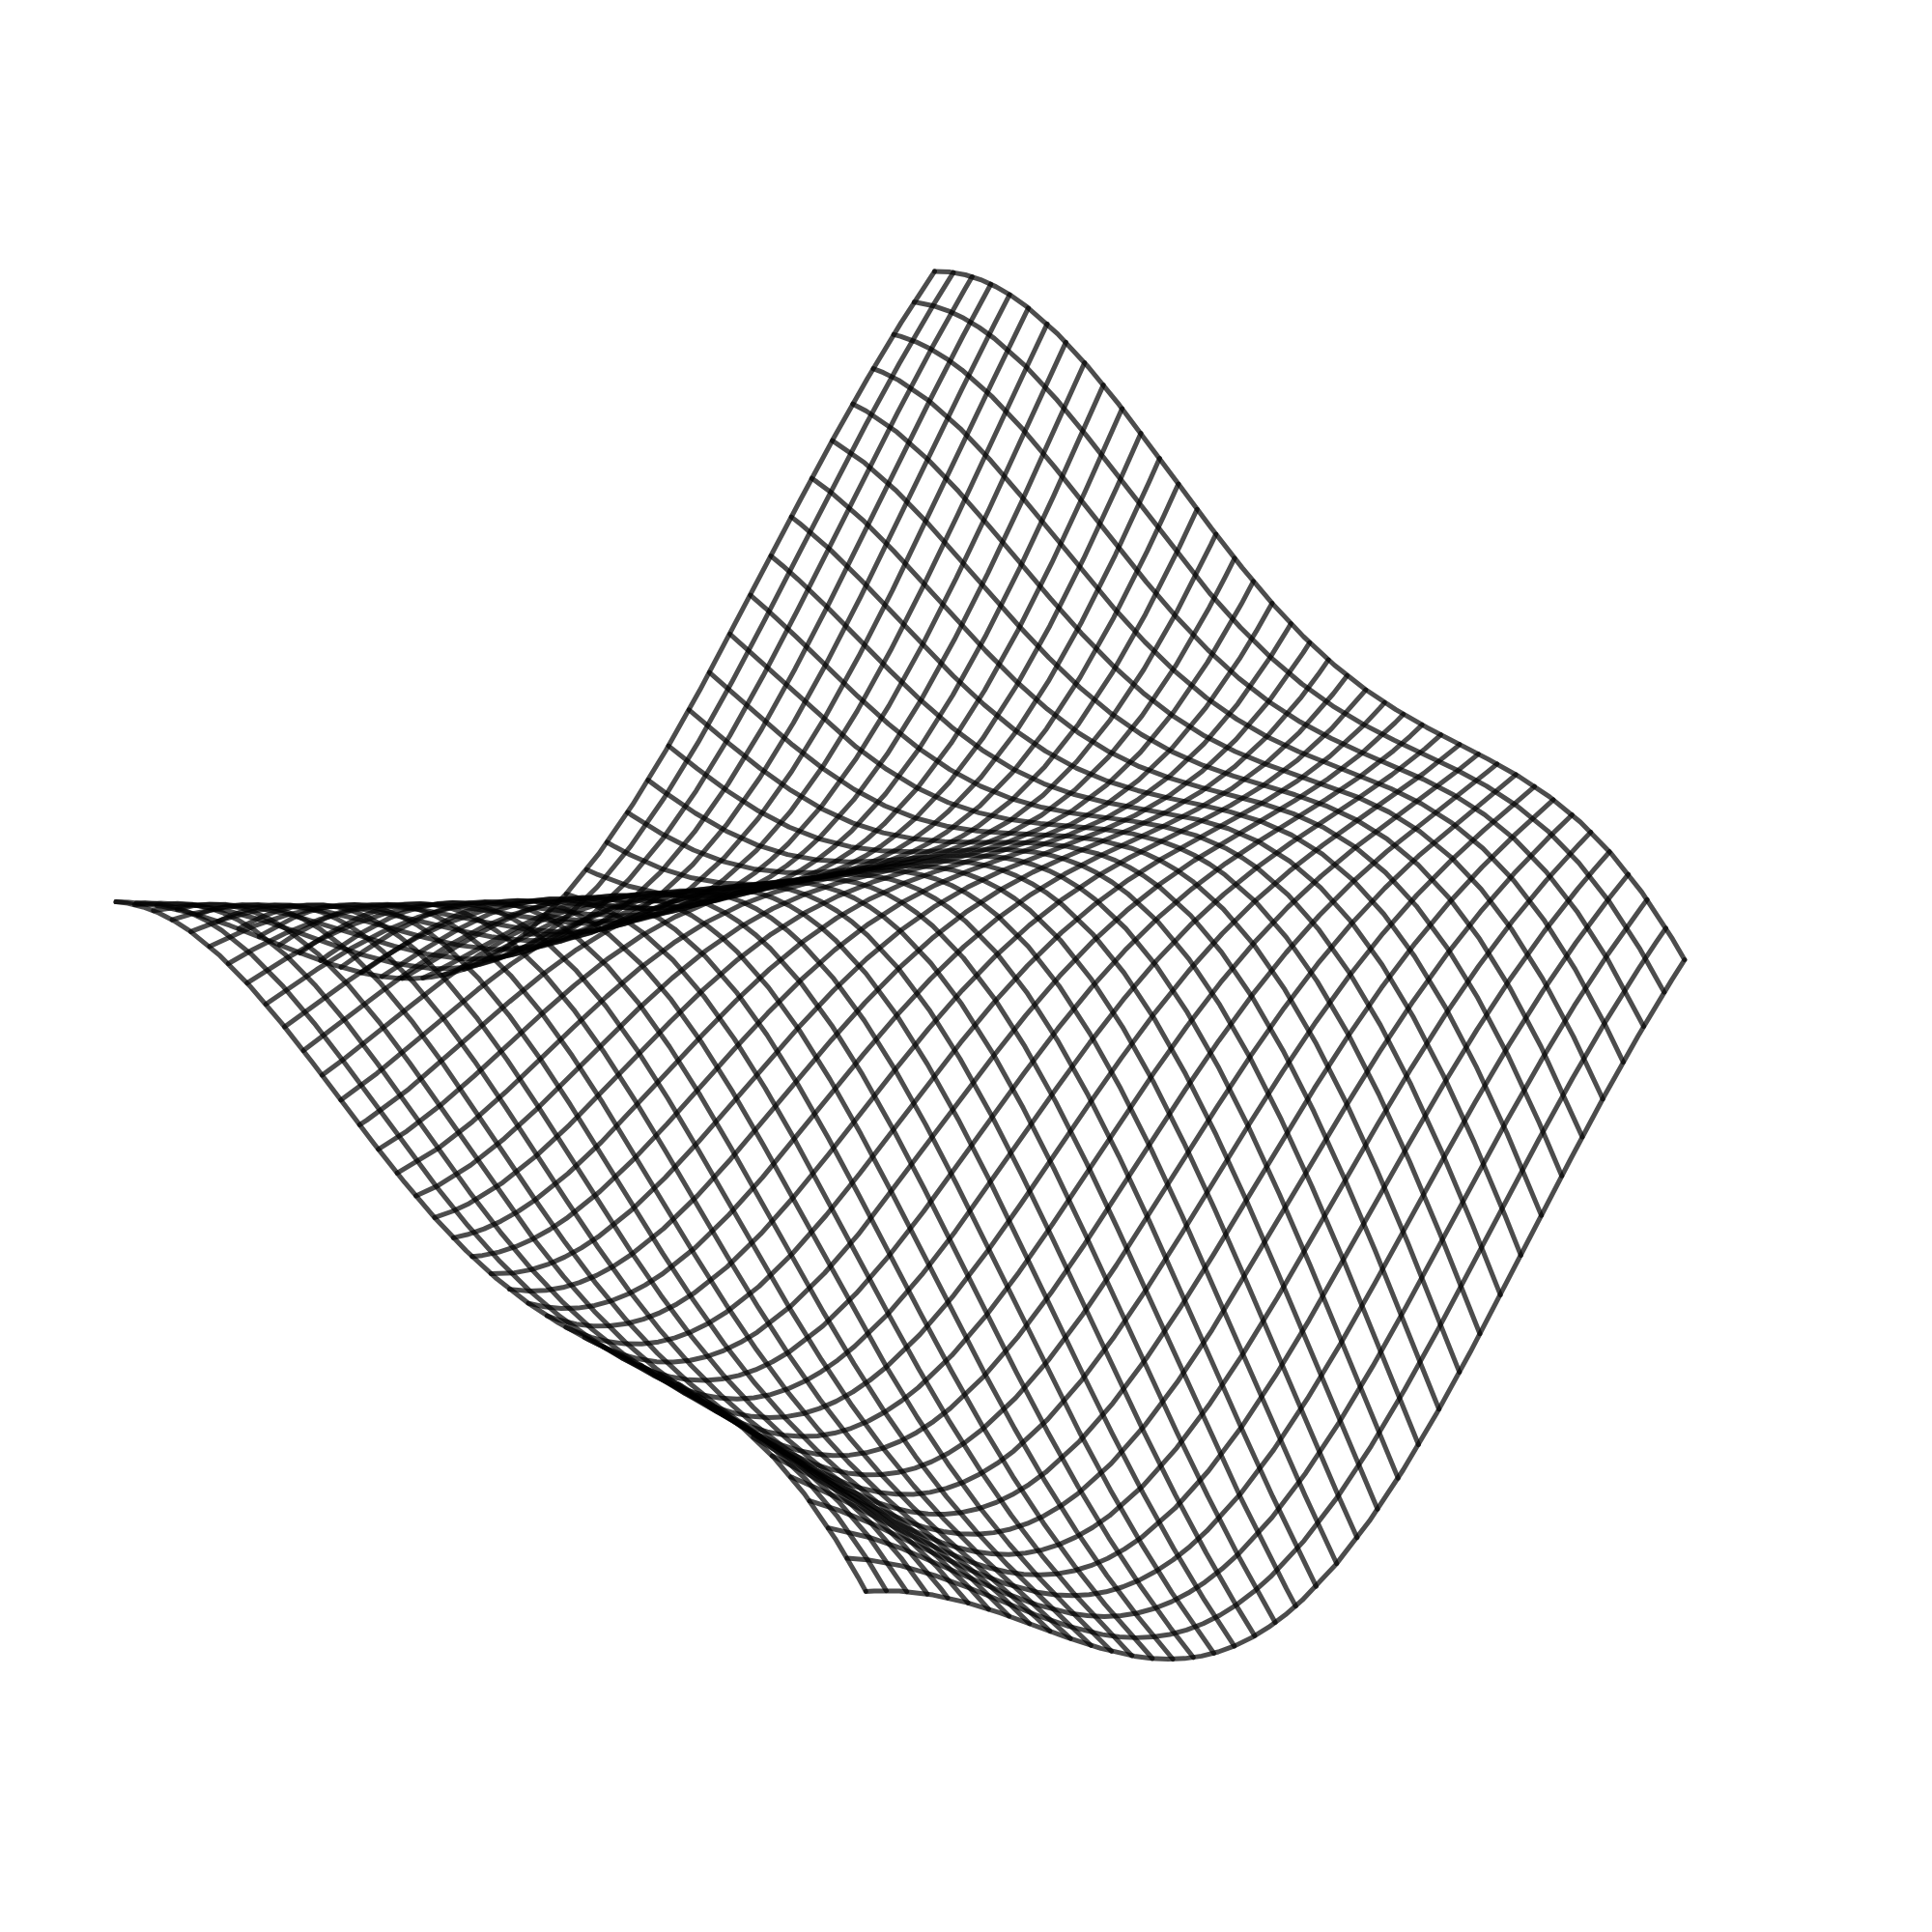
\includegraphics[width=0.9\linewidth]{img/m1/explicit.png}
  \caption{}
  \label{fig-explicit}
  \end{subfigure}
  \begin{subfigure}{0.5\linewidth}
    \centering
    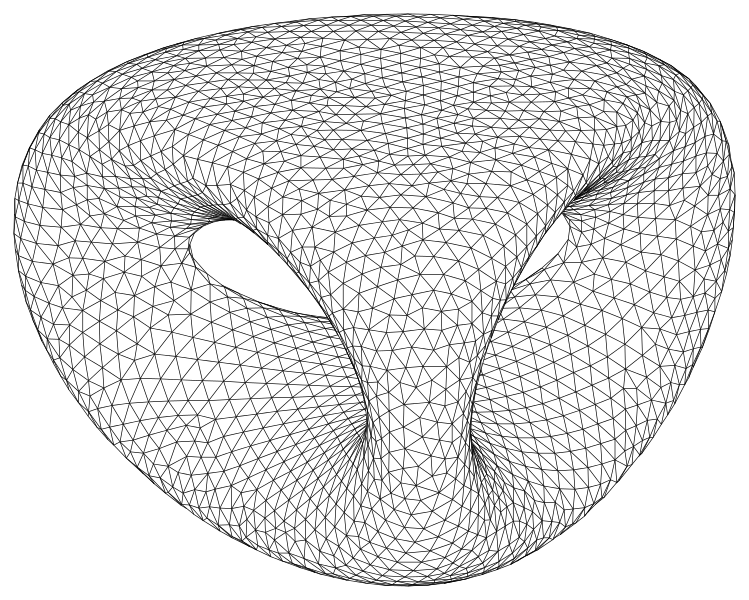
\includegraphics[width=0.8\linewidth]{img/m1/implicit.png}
    \caption{}
  \end{subfigure}
  \caption{(a) An explicit surface, given by $z = \cos ((x+y))+\frac{x^{2}}{6}-\frac{y^{2}}{6}$. (b) An implicit surface, given by $2 y\left(y^{2}-3 x^{2}\right)\left(1-z^{2}\right)+\left(x^{2}+y^{2}\right)^{2}-\left(9 z^{2}-1\right)\left(1-z^{2}\right)=0$. }
  \label{fig-imex}
\end{figure}

Apart from the explicit and implicit forms, surfaces can also be represented in their parametric form. The coordinates of a point $(x,y,z)$ of the surface patch are expressed as functions of parameters $u$ and $v$ in a closed rectangle:

\begin{equation}
x=x(u, v), \quad y=y(u, v), \quad z=z(u, v), \quad u_{1} \leq u \leq u_{2}, \quad v_{1} \leq v \leq v_{2}.
\end{equation}

In vector notation, the parametric surface can be specified by a vector-valued function

\begin{equation}
\mathbf{r}=\mathbf{r}(u, v)
\end{equation}

The parametric representation of surfaces is the most versatile out of the three. It is axis independent and is highly flexible in terms of defining complex intersections and point classification. It is generally easier to manipulate free-form shapes in parametric form than implicit or explicit forms  \cite{patrikalakis2009shape}. Hence, most of the CAD packages use parametric form of the surfaces to manipulate them. Bezier surface patch is one example of parametric form of a surface. 

\subsection{Surface File Format}


\begin{figure}
  \centering
  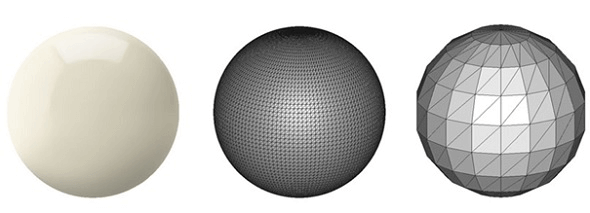
\includegraphics[width=\linewidth]{img/m1/tessellation.png}
  \caption{The perfect spherical surface on the left is approximated by tessellations. The figure on the right uses big triangles, resulting in a coarse model. The figure on the center uses smaller triangles and achieves a smoother approximation \cite{fileFormat}}
  \label{fig-tesellation}
\end{figure}

Given a free-form 3D surface geometry, various CAD packages could be used to encode it and store it in a file. Encoding the geometry using an approximate mesh is one of the most common methods adopted to store a surface geometry. An approximate mesh is created by covering the surface geometry with a series of tiny imaginary polygons. Trianlges are the most common polygon used for mesh generation. The encoded surface mesh can be stored in a file for sharing and future reference purposes. These files store the vertices of the triangles as well as the outward normal directions to the triangles. This process of tiling a surface with non-verlapping geometric shapes is also known as tessellation. Hence, the file formats used for storing the surface representation are called tessellated formats.

Due to the independent development of various CAD packages, a plethora of surface file formats are present in the mesh generation ecosystem. Many of these formats, such as DWG file format by AutoCAD and BLEND file format by Blender are proprietary. Hence, many of these cannot be shared between people working on different CAD packages. Native file formats are used to solve this problem. These formats can be shared easily among people working on different meshing softwares. One of the most common neutral surface file format is the STL (STereoLithography) file format. This format is compatible with most of the CAD and visualization softwares. Hence, we use the STL file format to import the surface geometry into our mesh generation algorithm.

An STL file stores the surface as a triangulated mesh. The following information is stored for all the triangles in teh STL file format:

\begin{enumerate}
  \item The coordinates of the vertices
  \item The components of the unit normal vector to the triangle pointing outwards with respect to the 3D model
\end{enumerate}

Innumerable software packages are available online which can be used to triangulate a surface (see \cite{meshSoftware} for a list of such softwares). A fine triangular mesh can be considered as an approximate encoding of a given surface geometry. The approximation could be improved by increasing the number of triangles or decreasing their size. However, using smaller triangles results in larger number of triangles needed to tile the surface. This increases the mesh file size. Hence, a user should define the mesh element size according to the kind of refinement needed.

\section{Surface Import and Segmentation using Common Geometry Module (CGM)}

As explained earlier, we import the surface geometry as a triangulation as an STL file. The Common Geometry Module (CGM) package is used to read the surface file and store the triangulation for further processing. The triangulated surface is stored as a collection of segmented sub-surfaces. The segmentation in CGM is done by identifying features in the surface. The only input parameter for surface segmentation accepted by CGM is the feature angle. We keep this feature angle value to be 135{$^\circ{}$}. This value helps us to identify sharp corners and edges on the surface. Figure \ref{fig-surfSegment} shows a surface triangulation of an arbitrary mechanical part. The surface triangulation is segmented into 10 sub-surfaces, which are identified by the sharp features on the surface. Four of these are shown in outline in the figure.

Each triangle imported in CGM is stored as a quartic-bezier patch. We will refer to the imported triangulation as $T$ and the underlying bezier surface representation as $S$. The underlying bezier surface representation $S$ is considered to be the ground truth for the surface and the mesh points are placed directly over $S$. Initial imported triangulation $T$ is taken as the initial mesh. We use a closed advancing layer mesh generation methodology. There are advantages and disadvantages of using such a methodology. Open advancing layer method requires less work overall to generate the mesh as there are no points to delete or reconnect to, ahead of the front. On the other hand, handling mesh layer collisions is  more tricky in open advancing layer method as no connectivity information is available ahead of the front in such methods. This leads to abrupt layer closures, which are undesirable in an anisotropic mesh.

Closed advancing layer mesh generation method generates a valid surface mesh at any point in the mesh generation process. Hence, there is more flexibility in terms of when to stop the marching layers and output the mesh in its current state. Additionally, connectivity information is known ahead of the front. This information is helpful while tackling layer collisions. This will be explained in more detail when we talk about handling front collisions in *ref*.

\begin{figure}
\centering
\begin{subfigure}{.5\textwidth}
  \centering
  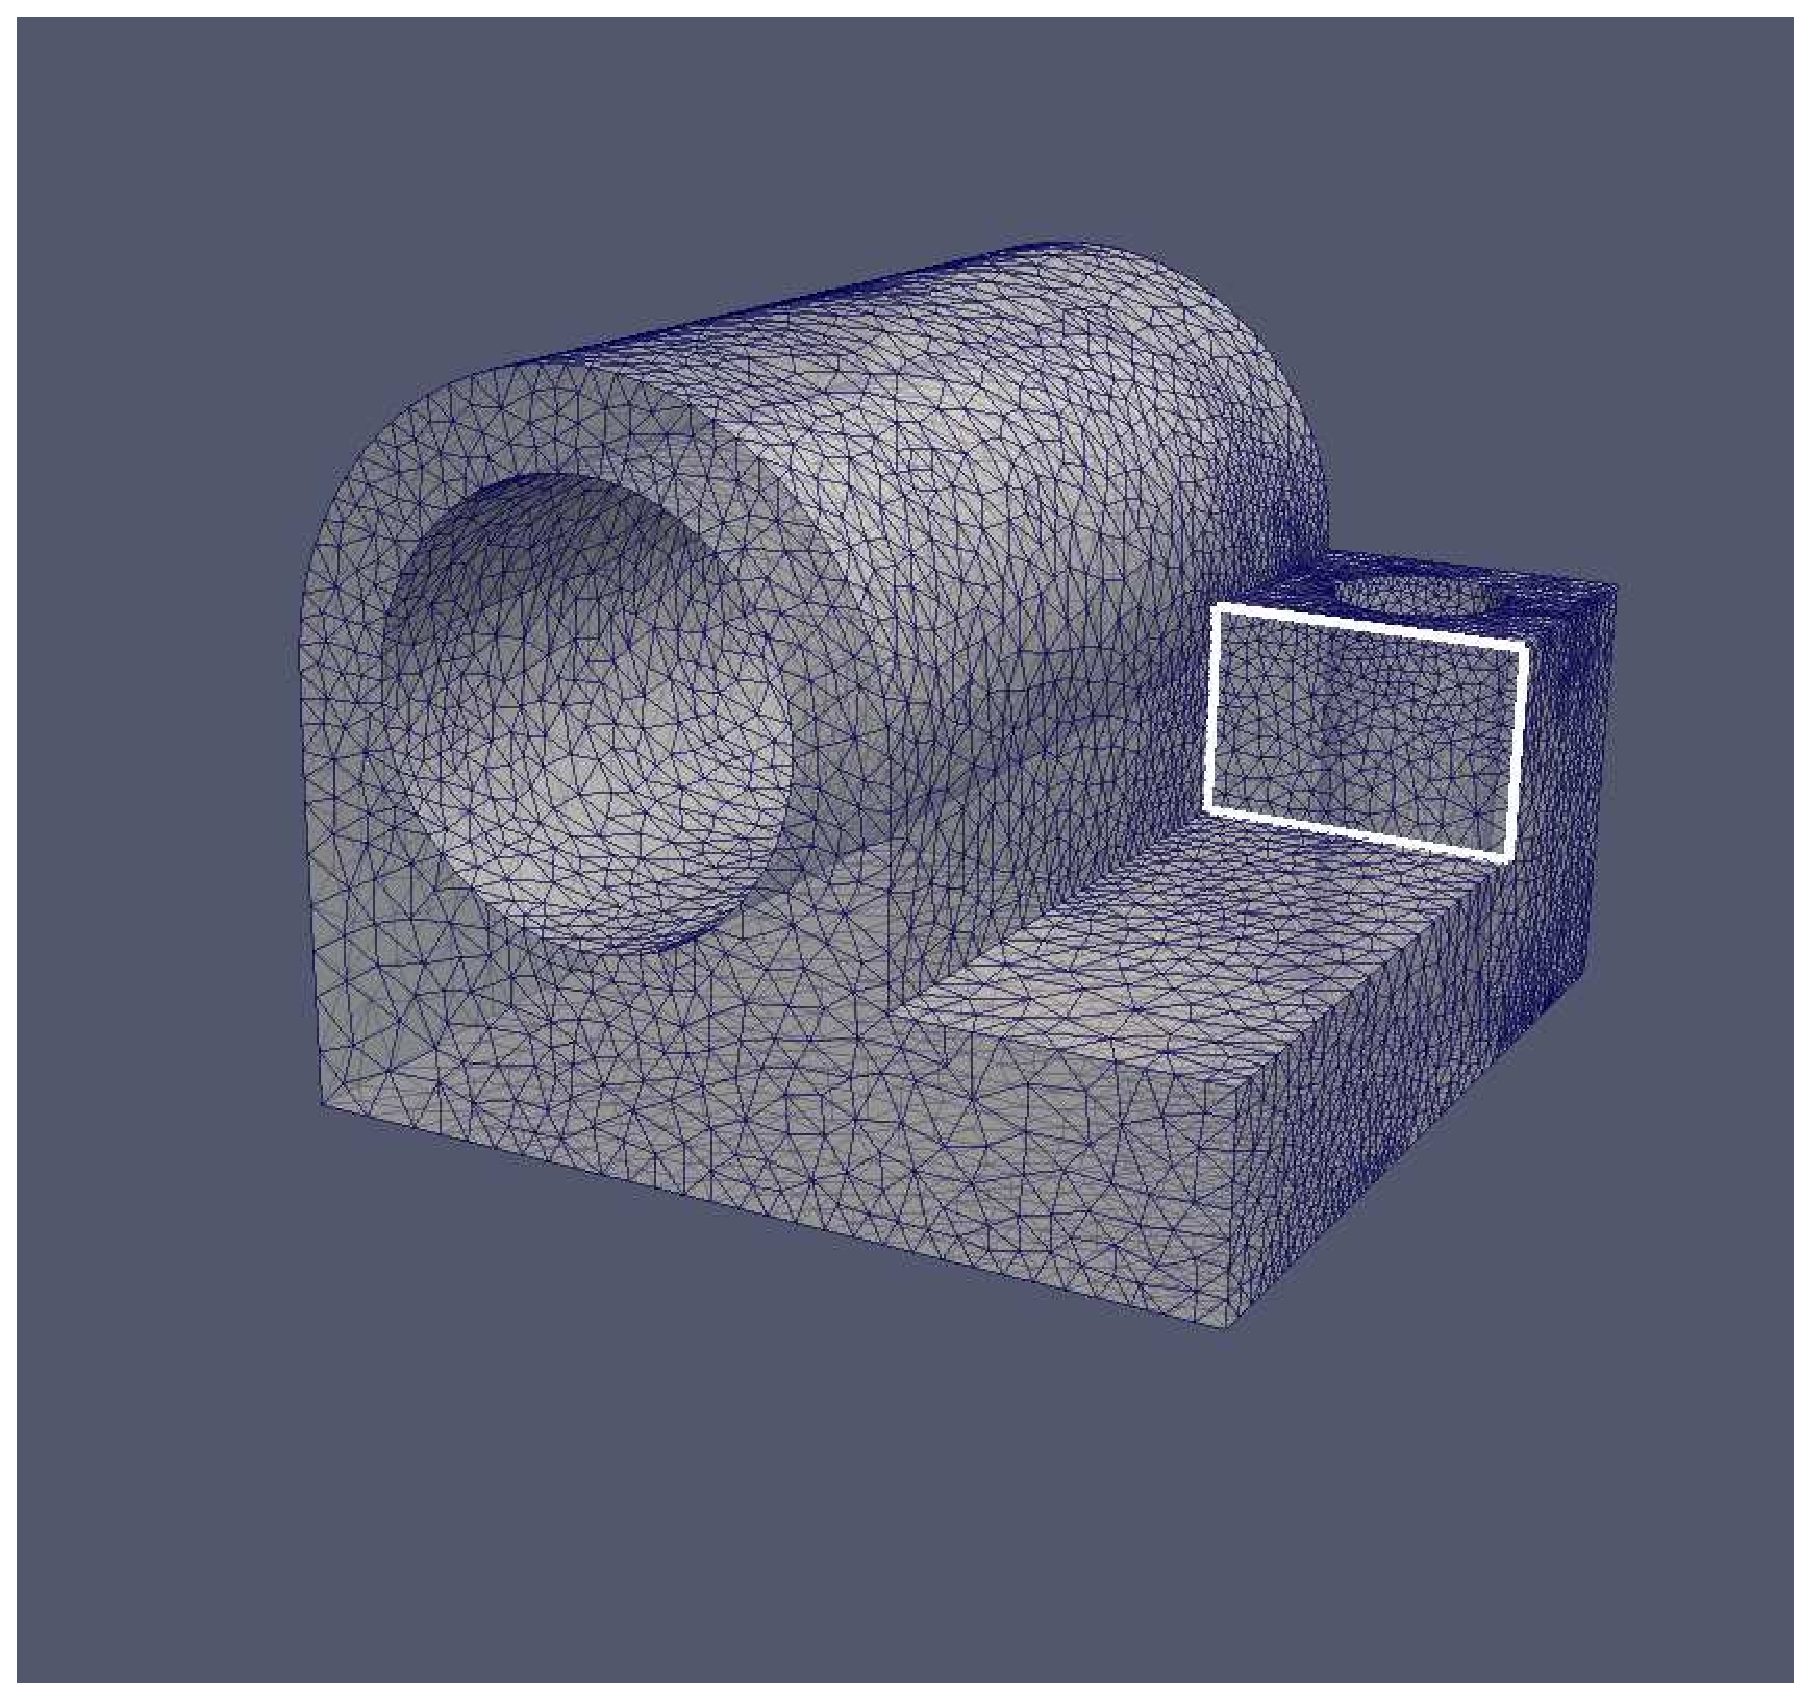
\includegraphics[width=.8\linewidth]{img/m1/surfSegmentation/surf0.eps}
  \caption{}
  \label{surf0}
\end{subfigure}%
\begin{subfigure}{.5\textwidth}
  \centering
  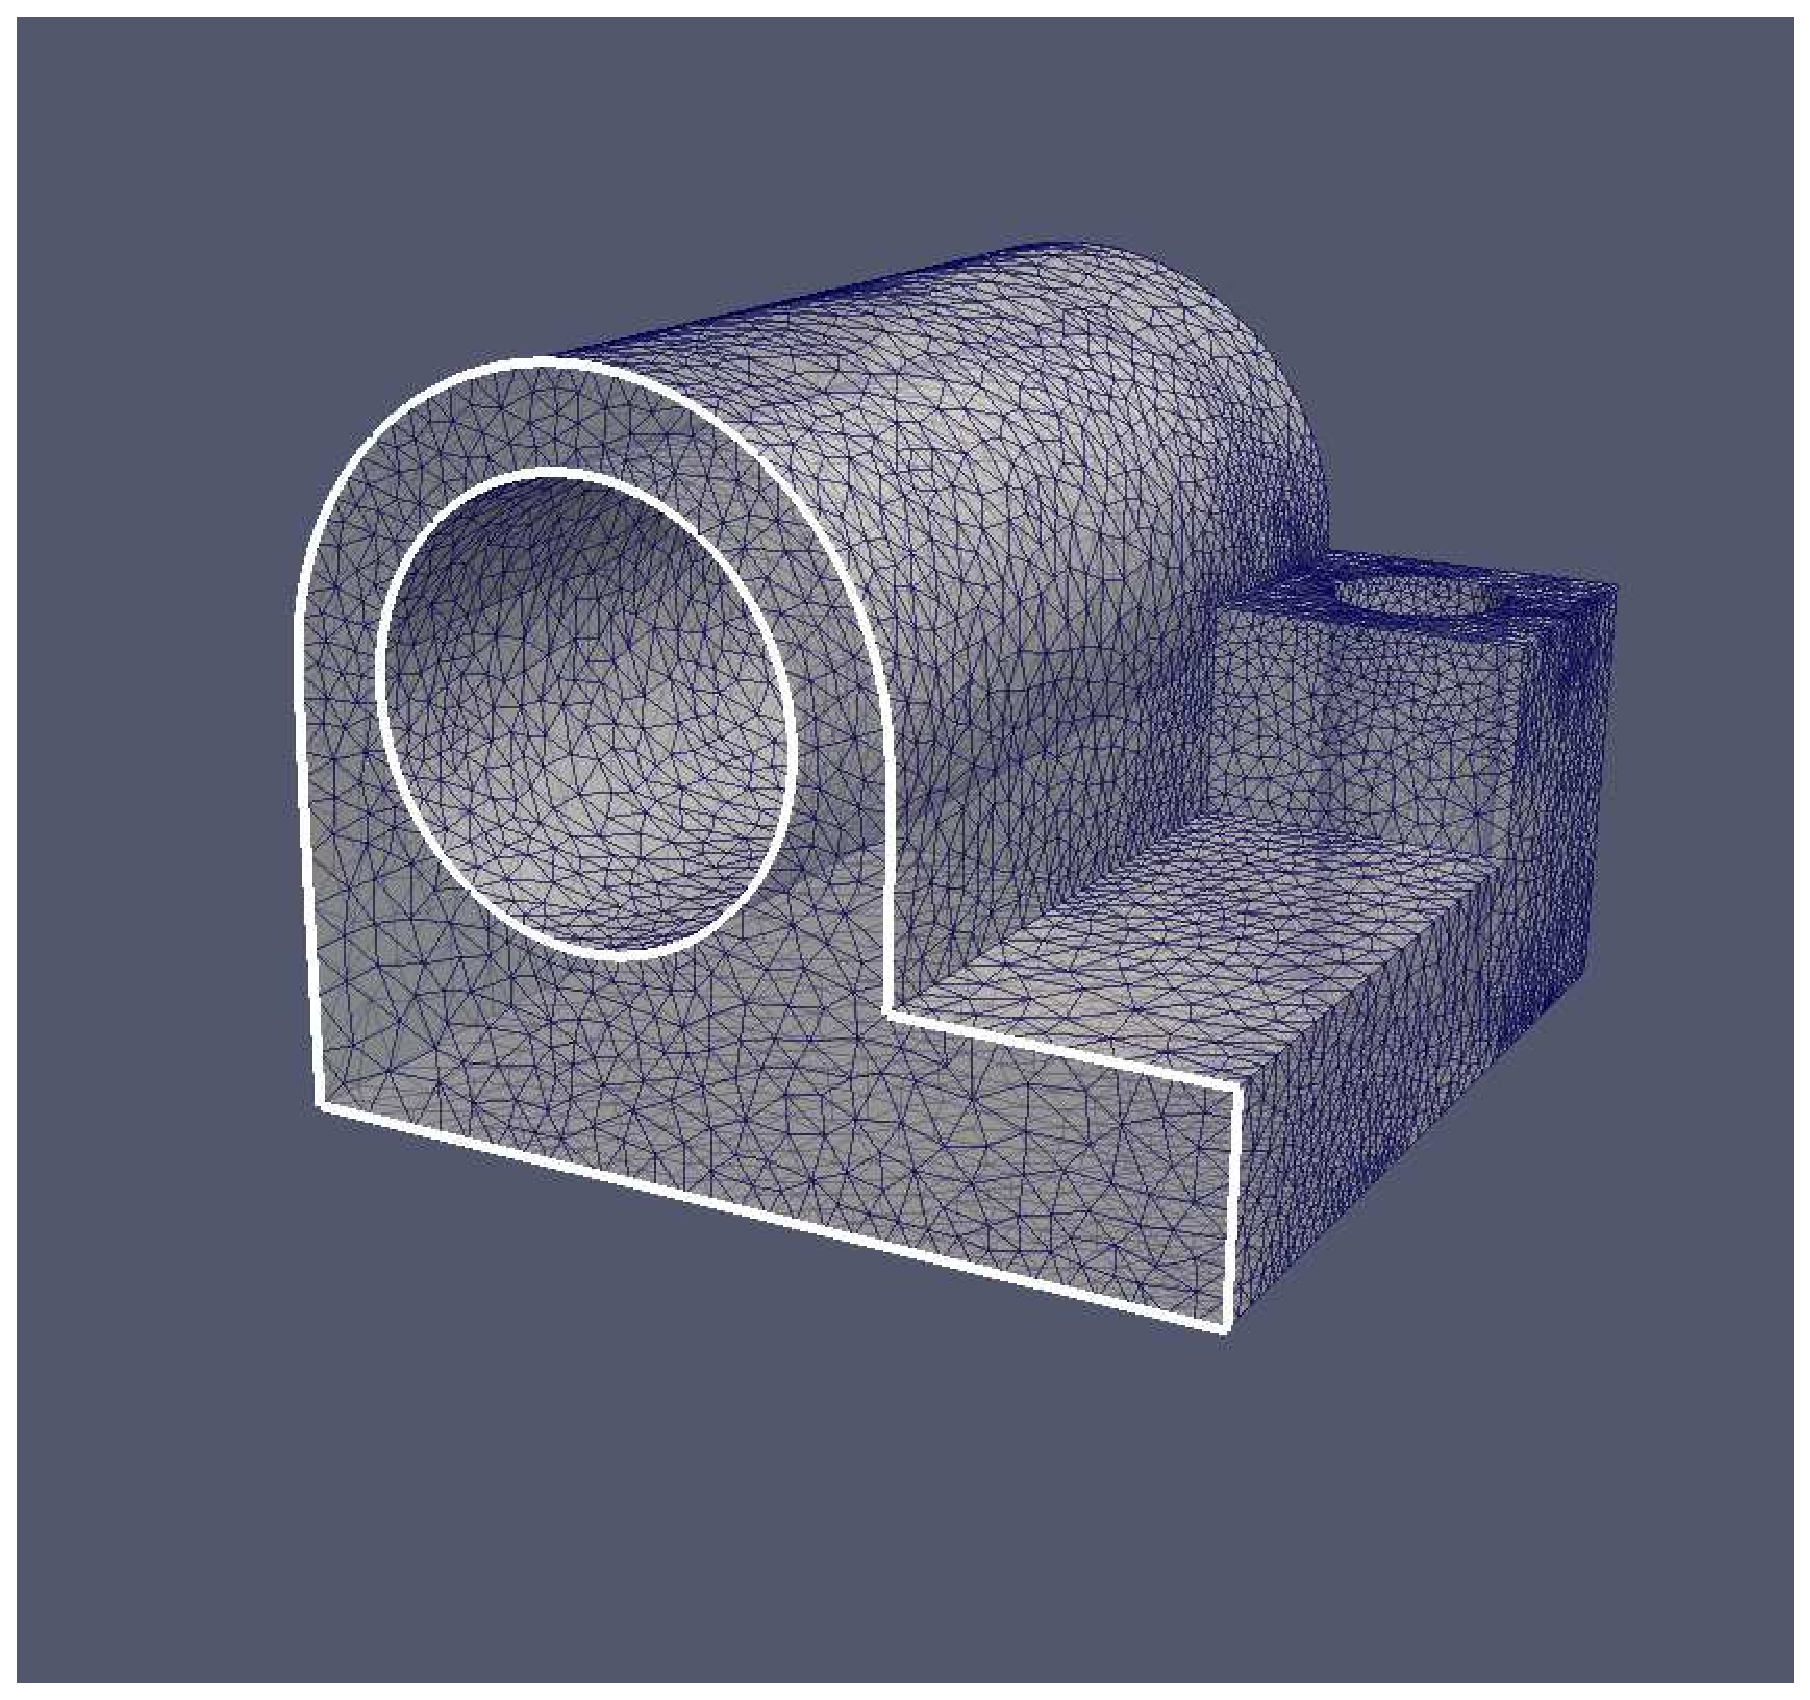
\includegraphics[width=.8\linewidth]{img/m1/surfSegmentation/surf3.eps}
  \caption{}
  \label{surf1}
\end{subfigure}
\begin{subfigure}{.5\textwidth}
  \centering
  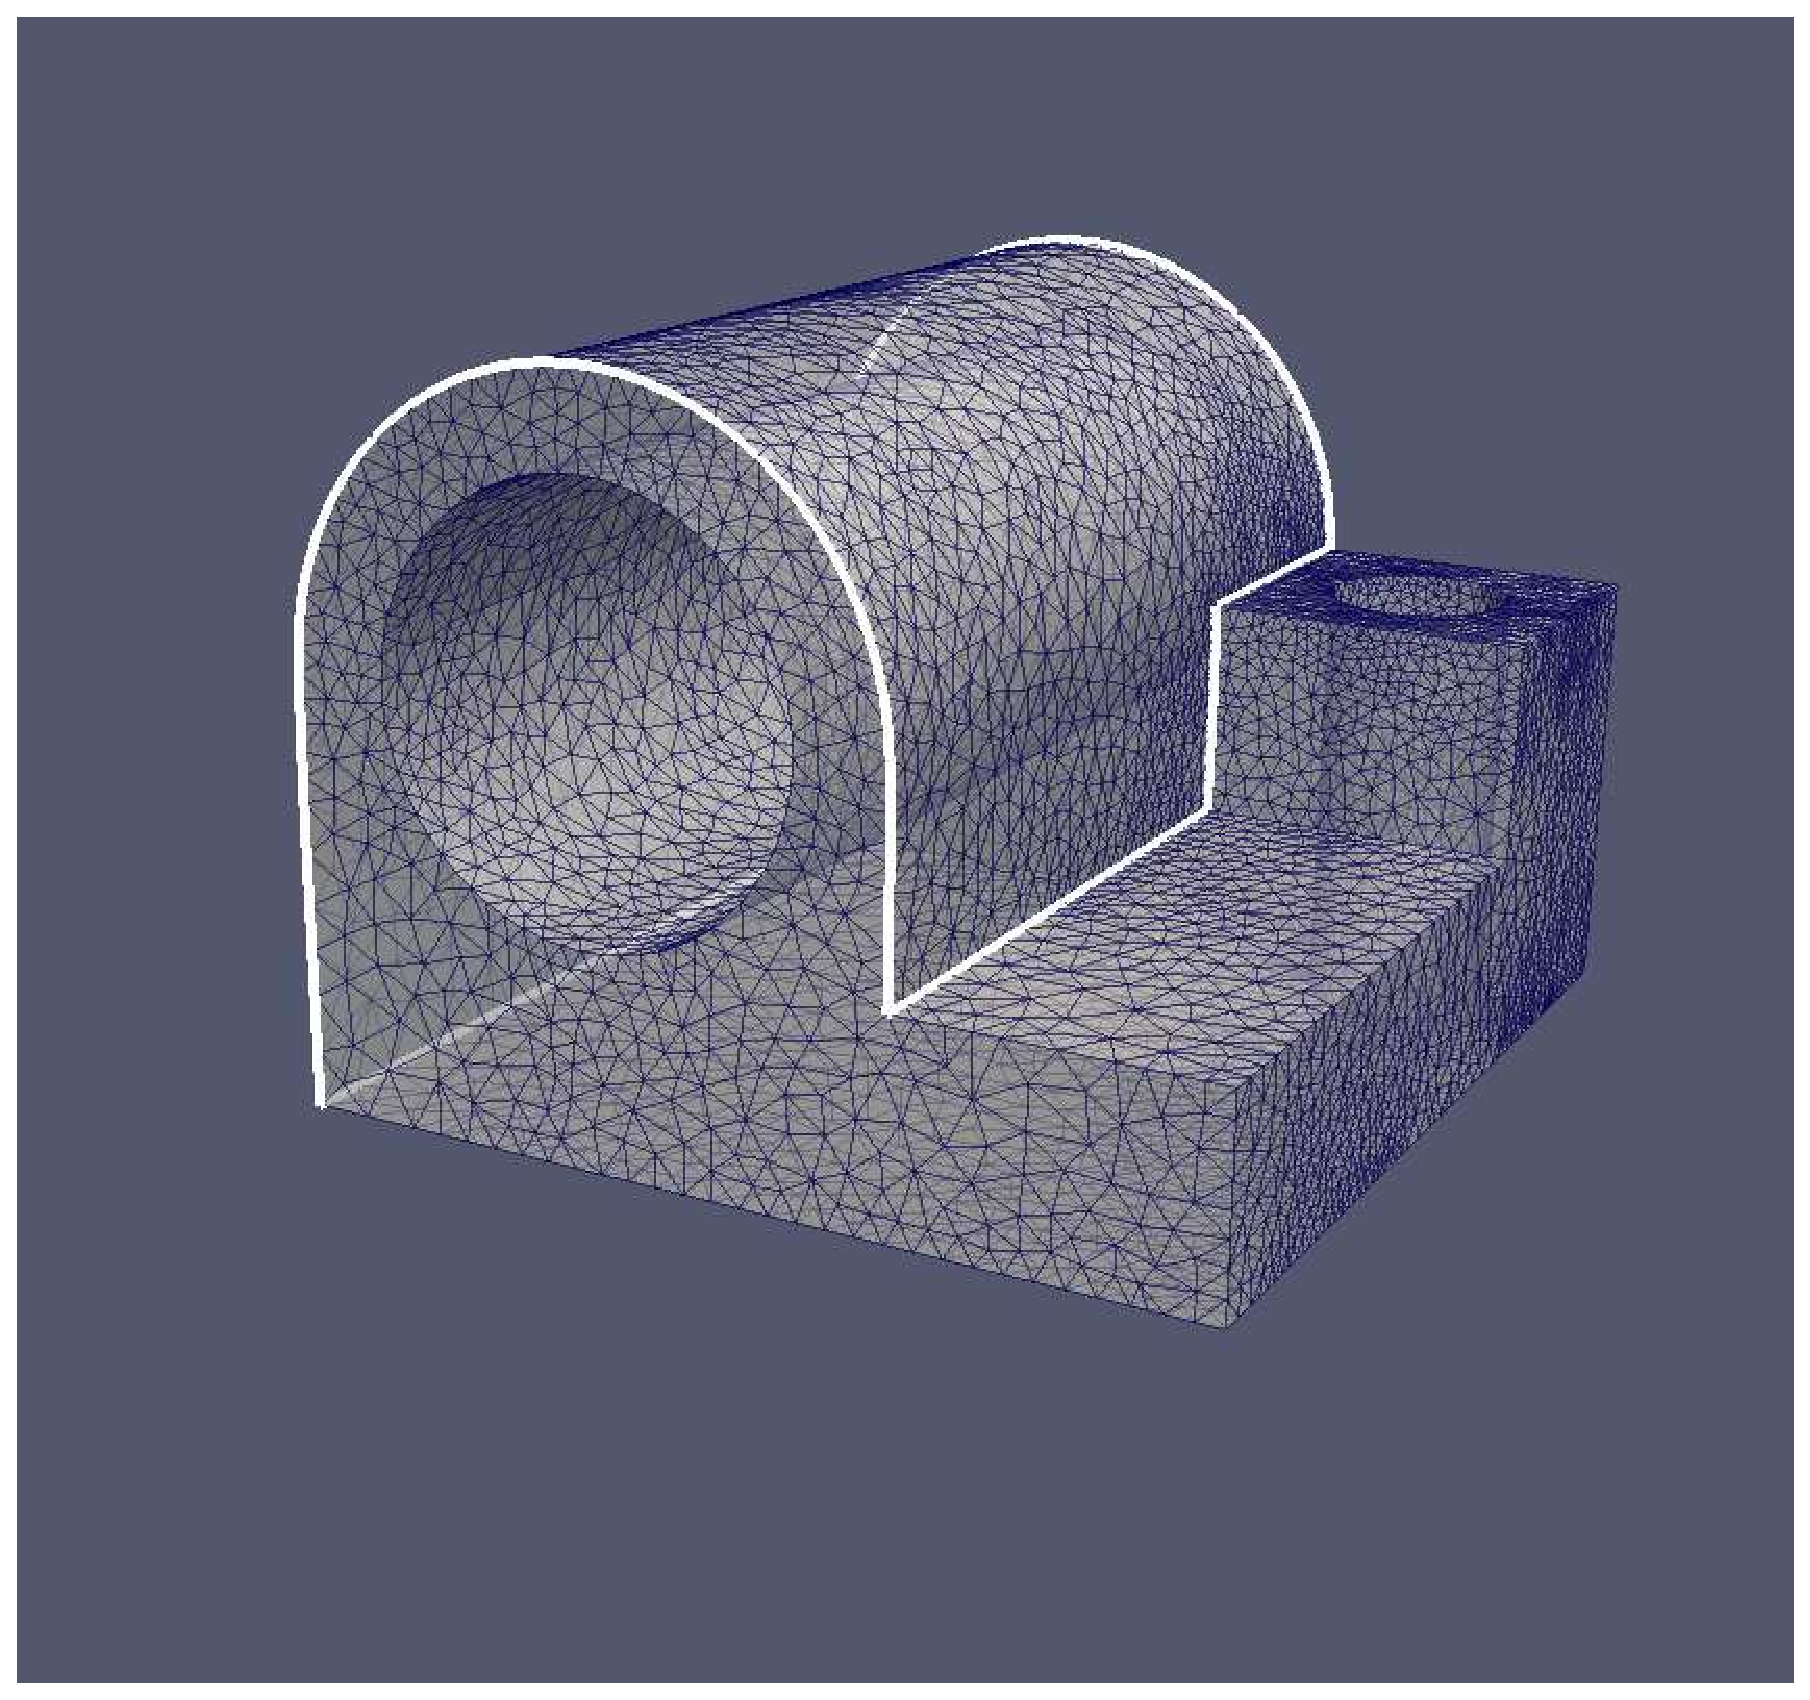
\includegraphics[width=.8\linewidth]{img/m1/surfSegmentation/surf5.eps}
  \caption{}
  \label{surf2}
\end{subfigure}%
\begin{subfigure}{.5\textwidth}
  \centering
  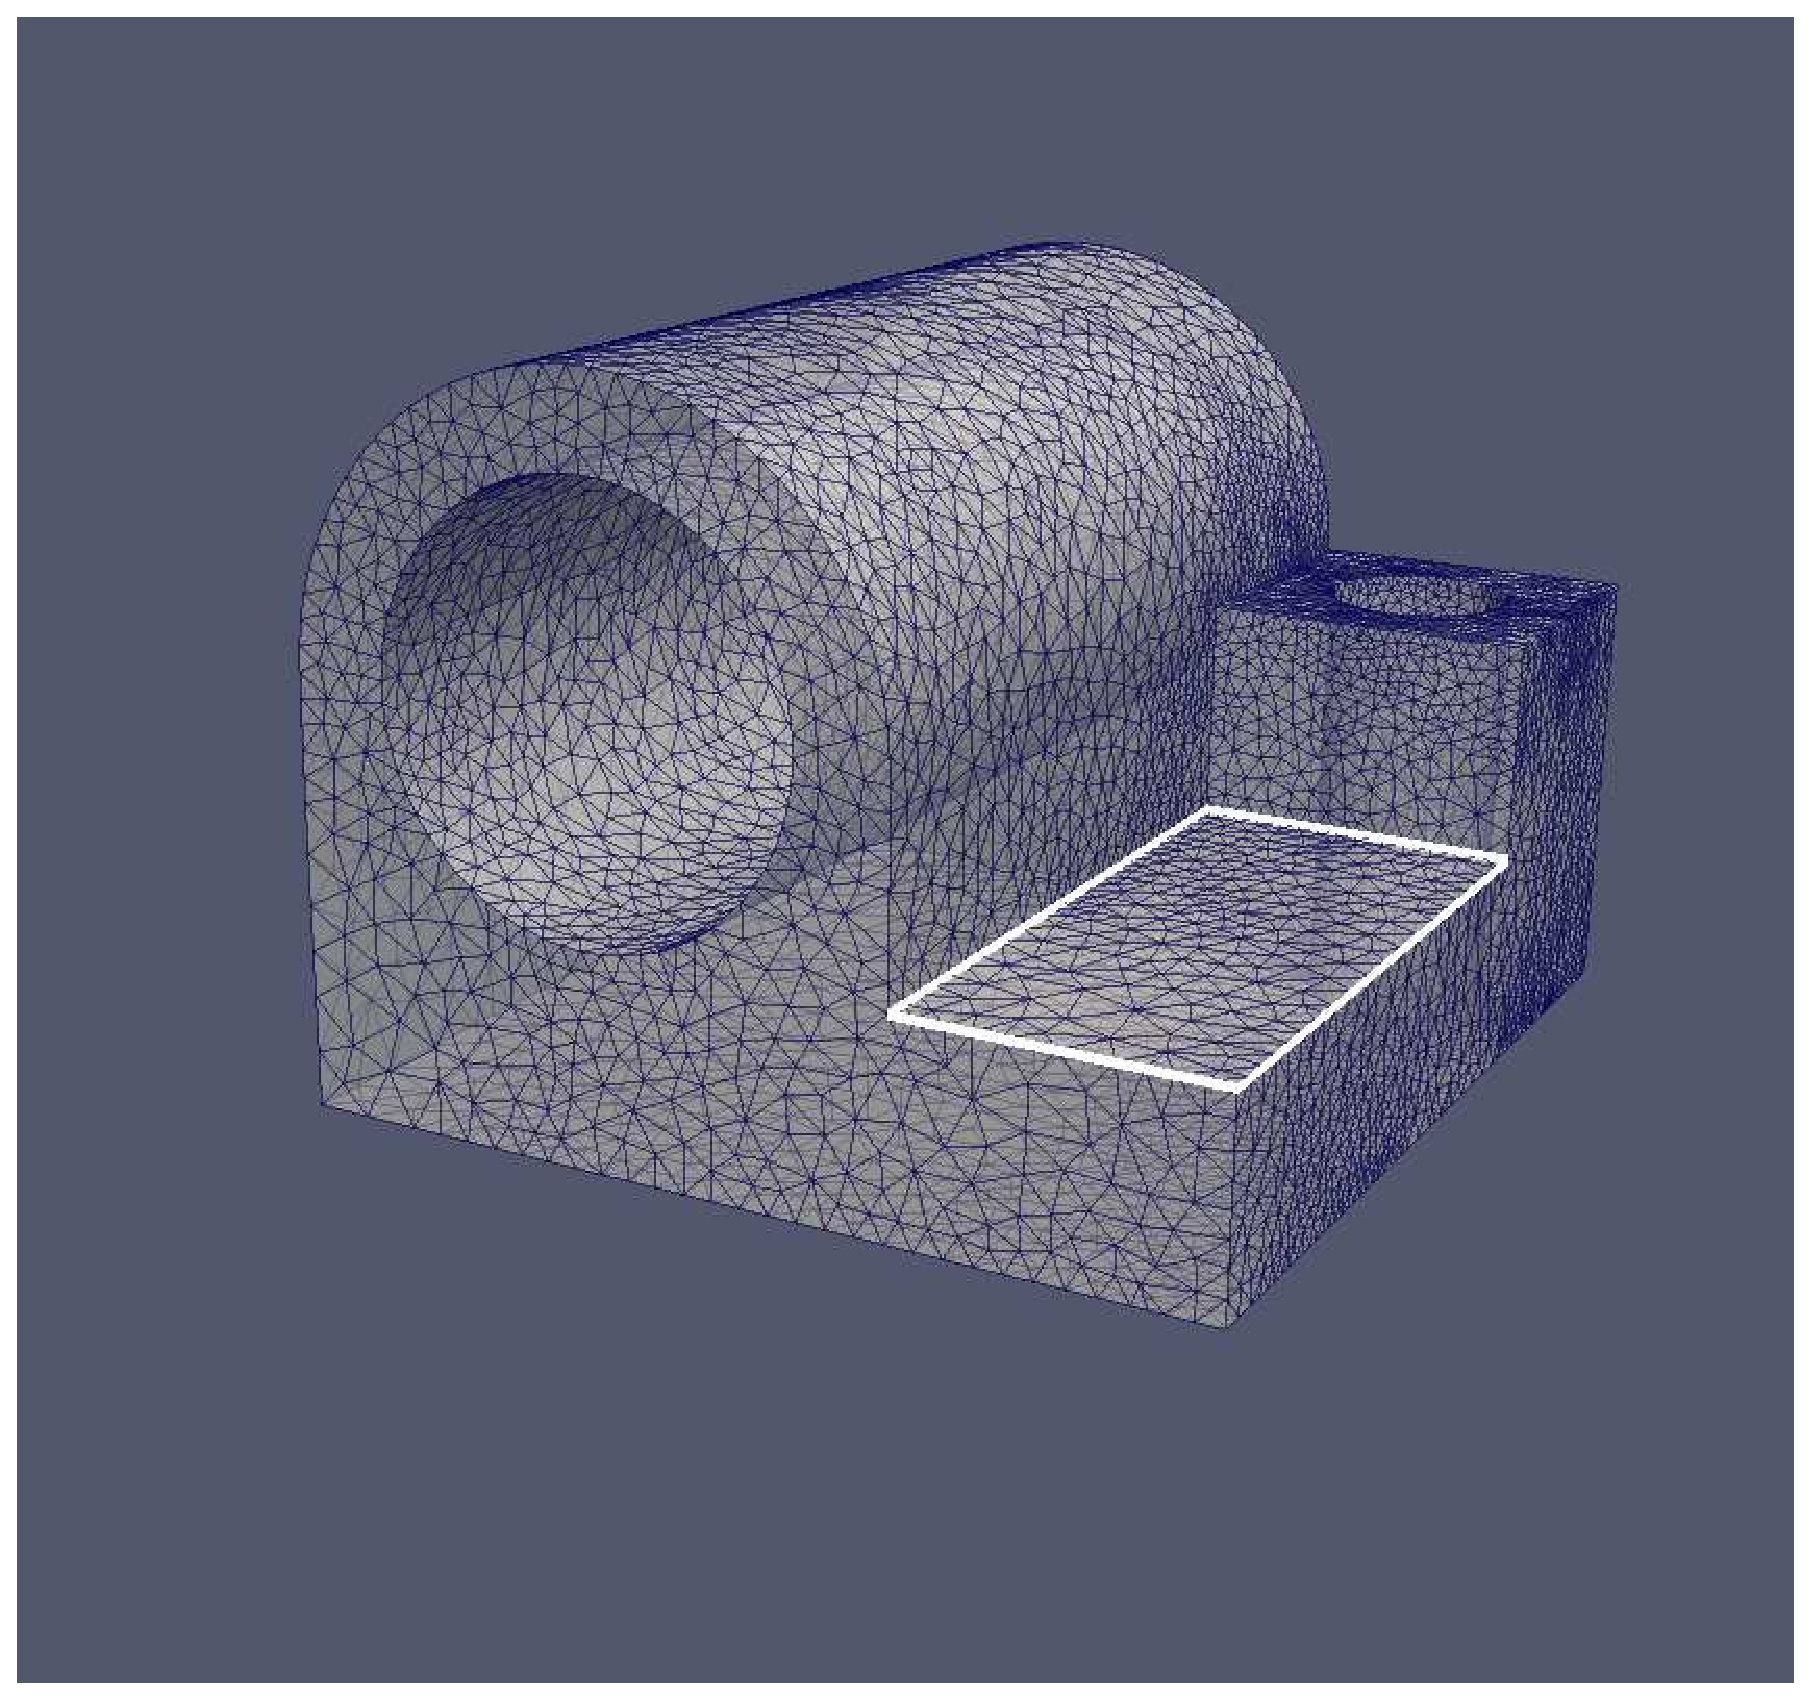
\includegraphics[width=.8\linewidth]{img/m1/surfSegmentation/surf7.eps}
  \caption{}
  \label{surf3}
\end{subfigure}
\caption{An example input triangulation of an arbitrary mechanical part. Four of the segmented surfaces are outlined.}
\label{fig-surfSegment}
\end{figure}

\subsection{Advancing Layer Initialization}

Sharp features of the imported surface are used by CGM to segment the surface. The boundary curves of the segmented surface denote these sharp features. For the purpose of this thesis, we consider these identified boundary curves as the initial front of the mesh. In other words, the boundary curves of the segmented surfaces (or sub-surfaces) serve as the zeroth layer of the advancing layer surface mesh.

Picking the boundary curves of the sub-surfaces to serve as the initial front helps us create anisotropy normal to these boundary curves. This way, desired refinement can be obtained normal to these boundary curves, which is a desirable feature as these boundary curves define the surface features. The discretization of the boundary curves imported along with the surface triangulation defines the refinement and gradation along the boundary curves (or along the zeroth front). Hence, the refinement and gradation along the boundary curves of the surface is defined by the input triangulation and is up to the user to vary. The surface mesh generated by EDAM-S hence provides with anisotropy along the normal direction (on the surface) to these boundary curves of the sub-surfaces.

We chose the boundary curves identified by CGM to serve as the zeroth layer of EDAM-S. However,the initial front could be chosen to be something else without affecting the rest of the mesh generation procedure. For eg. curves along high principal curvature directions on the surface could be added to the zeroth layer of the mesh to get the required anisotropy along highly curved regions of the surface. This is a work in progress and might be added to EDAM-S in the future.

\section{Point Placement}

After importing the surface triangulation, we have a valid underlying surface representation with us. Also, segmented sub-surfaces and their boundaries curves provide us with the boundaries we need to march off of. Each vertex on these boundary curves is extruded in two directions, one each for the sub-surfaces which share the boundary point. To make things simpler, two copies of each boundary vertex (vertex on the boundary) are created and associated with the two sub-surfaces which share the vertex. This untangles the process of generating the surface mesh of the two sub-surfaces, which now can be meshed independently. Meshing sub-surfaces independently has several advantages. If one sub-surface mesh fails to generate, other sub-surfaces would still continue to generate the advancing layer mesh. Also, parallelisation of the surface mesh generation subroutine would be simpler. From here onwards,  the discussion would focus on generating the mesh for a sub-surface, which is a segment of the complete surface. 

The mesh generation routine starts by initializing the front as the boundary curves of each sub-surface. All the boundary points are marked as candidate marching points and form the starting layer in the mesh. The points at the boundary curves of the sub-surfaces serve as the parent points for the first layer inserted into the mesh.

The data structure created to store a vertex on the advancing front of the mesh also stores the edges adjacent to that vertex so as to identify the marching directions. Hence, the extrusion direction or marching direction of a point is obtained from the location of the vertex, its adjacent edges, and the underlying sub-surface which is being meshed. The 
extrusion direction calculation procedure is explained in detail in the next subsection. Each edge on the advancing layer stores the direction into the interior of the sub-surface it bounds with respect to the surface normal. In other words, the edge datastructure stores its orientation relative to the sub-surface associated with it. As the sub-segments sharing a common boundary are meshed independently, it is easy to identify the normal to an edge along the sub-surface for advancing the front in the mesh generation algorithm.

%\begin{lstlisting}[language=cpp,caption={Caption}, frame=bt, numbers=none]
%// Class defining a vertex on the advancing layer
%class edamSurfVert {
%public:
%  int index;  
%  
%}
%\end{lstlisting}

\subsection{Advancing Layer Routine- Point placement} \label{advancing-layer}

For each of the sub-surfaces of the geometry, the advancing layer routine iteratively picks a point from its boundary and extrudes it in a given direction. After evaluating the extruded point, we project the point onto the underlying surface. This process is set up to be of two steps for simplicity, accuracy and computational efficiency as will be explained later.

\begin{figure}
\centering
\begin{subfigure}{0.5\textwidth}
  \centering
  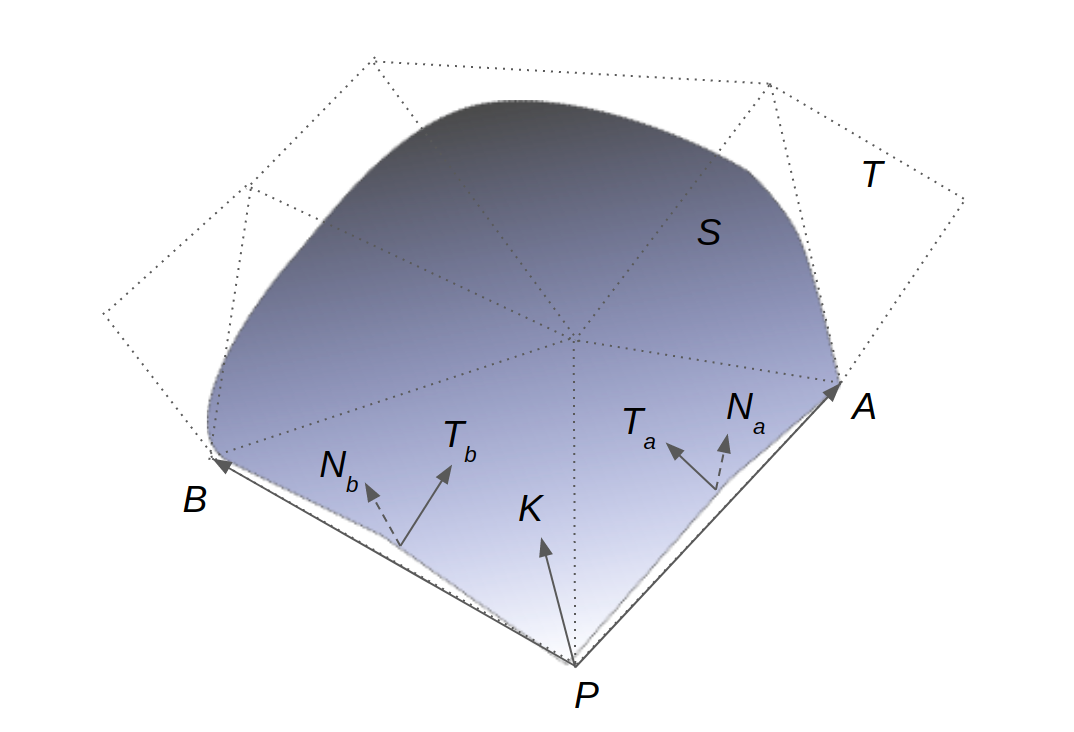
\includegraphics[trim={2cm 0 2cm 0},clip,width=\linewidth]{img/m1/pointPlacement.png}
  \caption{}
  \label{fig-pointPlacement1}
\end{subfigure}%
\begin{subfigure}{0.5\textwidth}
  \centering
  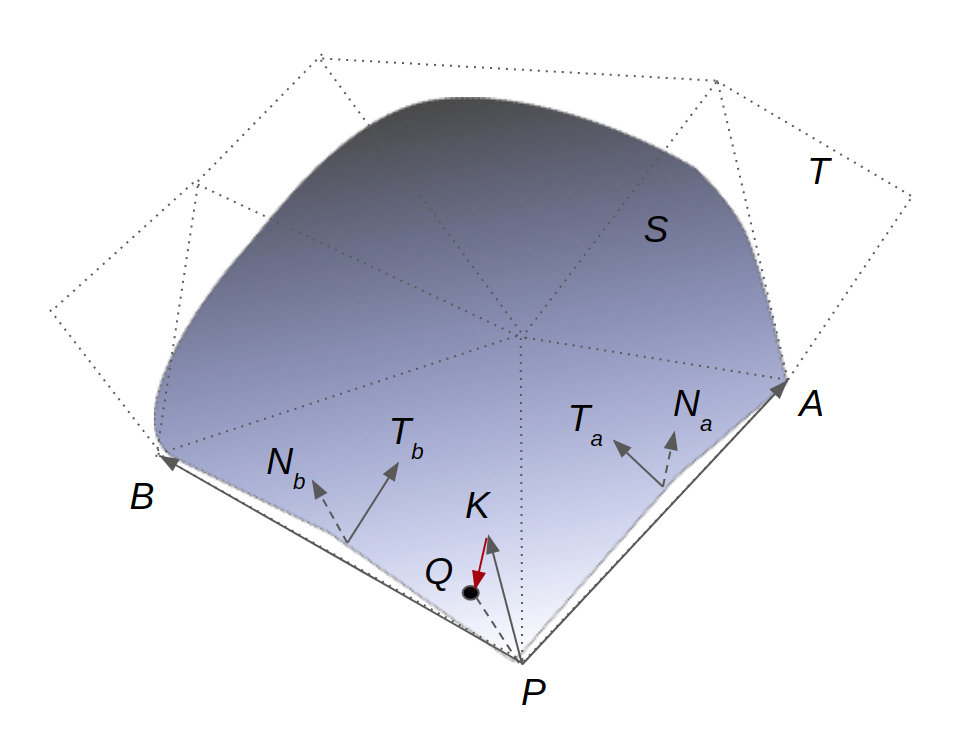
\includegraphics[width=\linewidth]{img/m1/pointProjection.png}
  \caption{}
  \label{fig-pointPlacement2}
\end{subfigure}
\begin{subfigure}{0.5\textwidth}
	\centering
	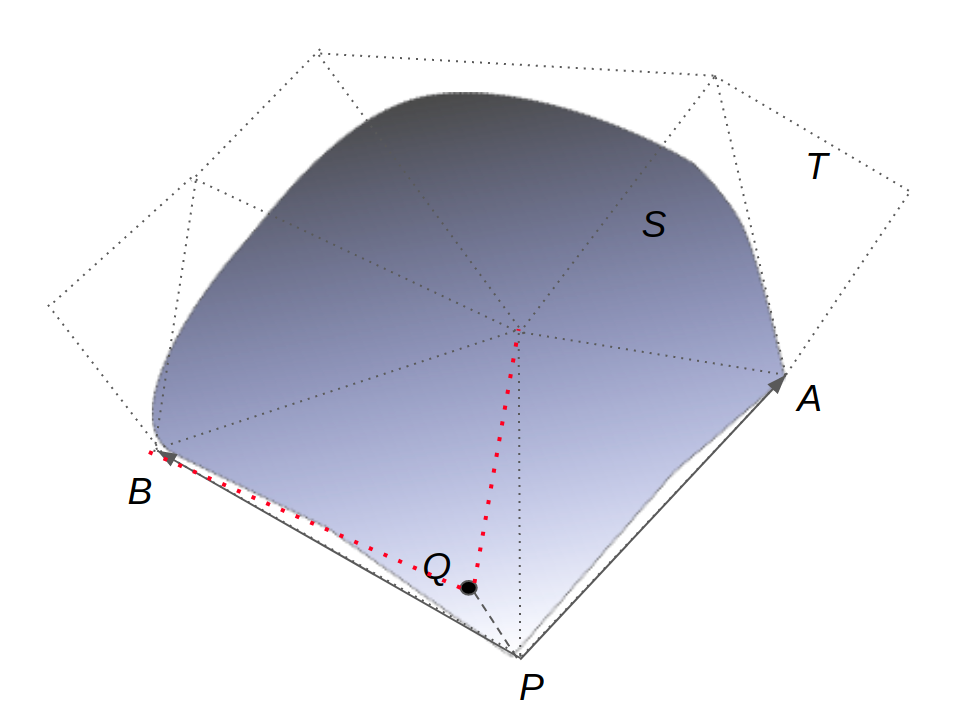
\includegraphics[width=\linewidth]{img/m1/pointInsertion.png}
	\caption{}
	\label{fig-pointPlacement3}
\end{subfigure}%
\begin{subfigure}{0.5\textwidth}
	\centering
	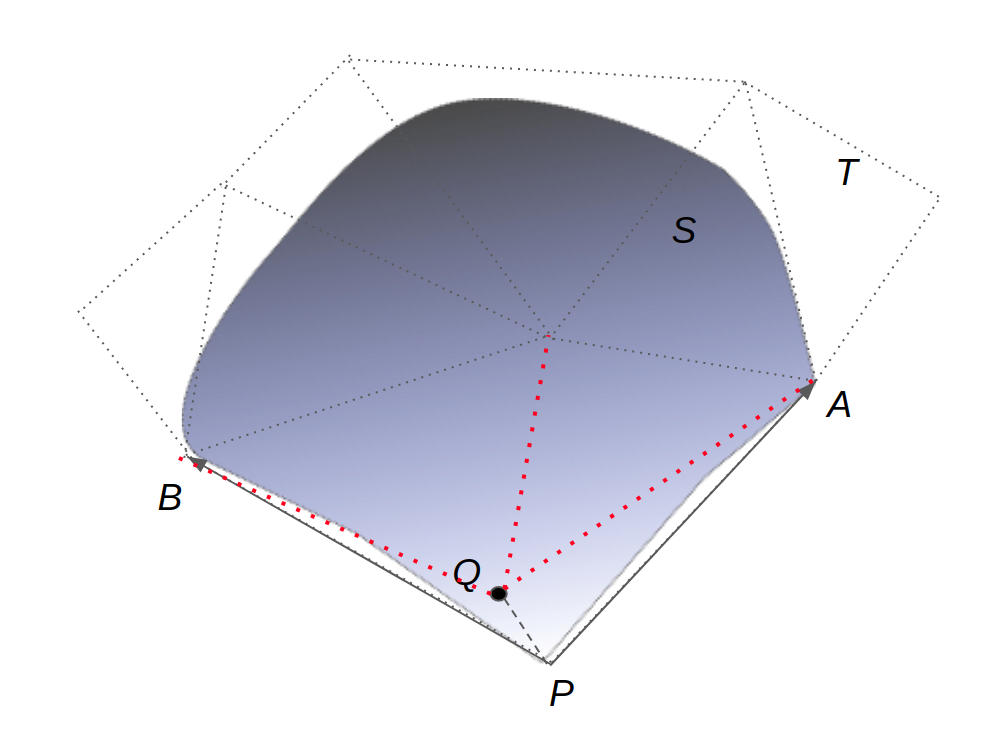
\includegraphics[width=\linewidth]{img/m1/localReconnection.png}
	\caption{}
	\label{fig-pointPlacement4}
\end{subfigure}
\caption{}
\label{fig-point}
\end{figure}

In the first step, we extrude the parent point to get the extruded point. We would interchangeably call the extruded points as the kid points as they represent the successors of their parent points from the previous layer. The direction of this extrusion is set up to be the average of the normals of the parent vertex's adjacent edges in the tangential plane of the sub-surface. In other words, the normals of the adjacent two edges of a vertex on the underlying sub-surface are averaged to get the extrusion direction.

Consider Figure \ref{fig-point}. Initial input triangulation is marked $T$ and the bezier surface representation is marked $S$. Point $P$ is at the boundary curve of the surface. We need to find the extrusion direction of P to know where its kid would be located. In the underlying triangulation $T$, $PB$ and $PA$ are the edges adjacent to $P$ on the boundary of the surface $S$. We first find the mid-points of quartic-Bezier curves $PB$ and $PA$ which are constructed by CGM as a part of constructing the quartic-Bezier triangular surface patches from the underlying triangulation $T$. Next, we find the normal directions on the surface at these mid-points. The normal directions are carefully queried from the sub-surface which is being meshed currently. The normal directions are labeled as $N_b$ and $N_a$ in the figure. We cross product the vector $PB$ with $N_b$ to get the direction $T_b$. The vector $T_b$ is normal to the edge $PB$ as well as tangential to the surface $S$. Similarly, we find the vector $T_a$. The direction of extrusion $\vec{PK}$ is chosen to be the average of the direction of $T_a$ and $T_b$.

The initial extrusion length is an input parameter provided by the user. This length would be taken as the extrusion length when the boundary points are extruded for the first time to the interior of the surface. This length can vary with boundary vertices as the points are extruded independently. Hence, this extrude length can either be supplied by the user for all the points of the boundary separately or as a single value for all the boundary points. To obtain best quality quad elements, we scale the extrusion length at a given vertex on the advancing layer with respect to the interior angle between the direction vectors $T_a$ and $T_b$. If the vertex is a concave corner vertex, the extrusion length is increased so as to create good quality quad elements in the next layer. This process is described in detail in section \ref{section-extrusionScaling}.%and vice-versa for convex corner vertices. Also, if the vertex is a convex corner, additional marching directions are added so as to sufficiently refine the interior domain of the surface. The number of additional marching directions added depends on the convexity of the vertex. If we have $n$ marching directions for a point, the angle between the adjacent edges would be divided into $n+1$ angles to get the marching directions for the $n$ points. We hope to include these modifications in the final paper submission.

After we have extruded the point, we project it on to the underlying geometry. This operation ensures that all the  points we insert in the mesh are on the underlying geometry. Errors here would compound in subsequent layers. Points are inserted in the mesh and the mesh elements are subdivided to include the new point. The candidate point for insertion can subdivide an existing triangle to replace the previous triangle with three new ones, or can subdivide an edge to replace existing two triangles with four new ones. To find the best triangle or edge for subdivision, we first make a guess for the triangle to insert the point. Any triangle in the surface interior adjacent to the point being extruded is chosen. Starting from this triangle, we iteratively jump to the best edge or triangle by comparing the barycentric coordinates of the new point with respect to the triangle in consideration. This technique suffers from two disadvantages. First, we need to compare double precision values of barycentric coordinates for making a decision on which triangle to choose for insertion. If the values are too close, the point might be inserted in the wrong triangle and would eventually lead to deviation of the mesh from the underlying surface. Second, the process of iteratively finding the right triangle for insertion might end up being in an infinite loop. Both of these problems are substantially reduced with a good isotropic initial triangulation. However, we add several validity tests to avoid these problems even for a coarse initial triangulation. These include orientation checks of the triangles formed with respect to the surface, thresholding the maximum deviation of the newly formed triangle from the surface and thresholding the dihedral angles between two triangles on the surface. We use an epsilon value of $10^{-5}$ while comparing the values of barycentric coordinates to zero. Also, we insert the point on a face rather than in a triangle when the ratio of the second-smallest barycentric coordinate to the smallest one is more than a set threshold ($10^2$). This helps us avoid very skinny triangles with large obtuse angles and also helps in avoiding several unnecessary face swapping in the mesh.

After advancing one layer to the surface interior, we increase the extrude length at each point by a factor. This factor, called the growth ratio, specifies the anisotropic layer-on-layer extrusion length growth as we march on the surface. A value of growth ratio between 1.1 and 1.4 gives us satisfactory anisotropy at the boundaries of the mesh.

%\begin{figure}
%    \centering
%    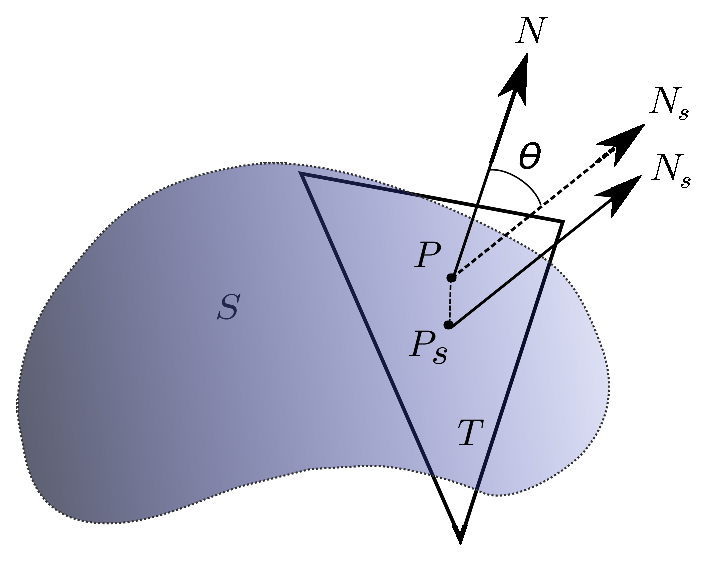
\includegraphics[width=.3\textwidth]{deviate-surface.eps}
%    \caption{Triangle $T$ deviates from the underlying surface $S$. $P$ is the centroid of $T$ and $P_s$ is the projection of $P$ on $S$. The deviation is calculated as the interior angle between the normal to the triangle $PN$ and the normal to the surface at $P_s$, which is $P_sN_s$. The angle $\theta$ represents the deviation here. The deviation is exaggerated for illustration purposes.}
%    \label{deviation-surface}
%\end{figure}

\section{Local Reconnection for quality}




%		3. Methodology 2 Advancing Several layers
\chapter{Methodology Part 2: Advancing Several Layers}

In the previous chapter, we talked about how the very first layer of the mesh is generated. Starting from the discussion of extruding one boundary vertex onto the sub-surface, we went on explained how all the vertices on the boundary curve of the sub-surface are extruded and subsequently, how the advancing front is recovered so as to move on to the next layer. We also talked about how extrusion length scaling at concave corners helps us avoid immediate front collapse and improves overall mesh quality. In this chapter, we are going to discuss some of the important subroutines which help complete the anisotropic surface mesh.

We will start by discussing the subroutine used to control the aspect ratio as we advance several layers in the mesh. Combining triangular mesh elements to quad elements would be discussed next. Subsequently, mesh smoothing and collision handling would be discussed.

\section{Aspect Ratio Control and Sub-surface Interior Improvement}

\subsection{Vertex Decimation on the Front}
\label{aspectRatioControl}

As the advancing front moves into the surface interior, the layers grow in size. This is done for the purpose of giving a higher refinement at the boundary curves. As the size of the layer grows, the aspect ratio of the mesh elements generated decrease. Also, some of the vertices on the front might come so close to each other that the aspect ratio approaches unity. Growing the layers further with all the vertices on the front would lead to anisotropy in the orthogonal direction  and/or front overlap. Hence, decimation of some of the front vertices is necessary to proceed with the next few layers.

\begin{figure}[hbt!]
\centering
\begin{subfigure}{.5\textwidth}
  \centering
  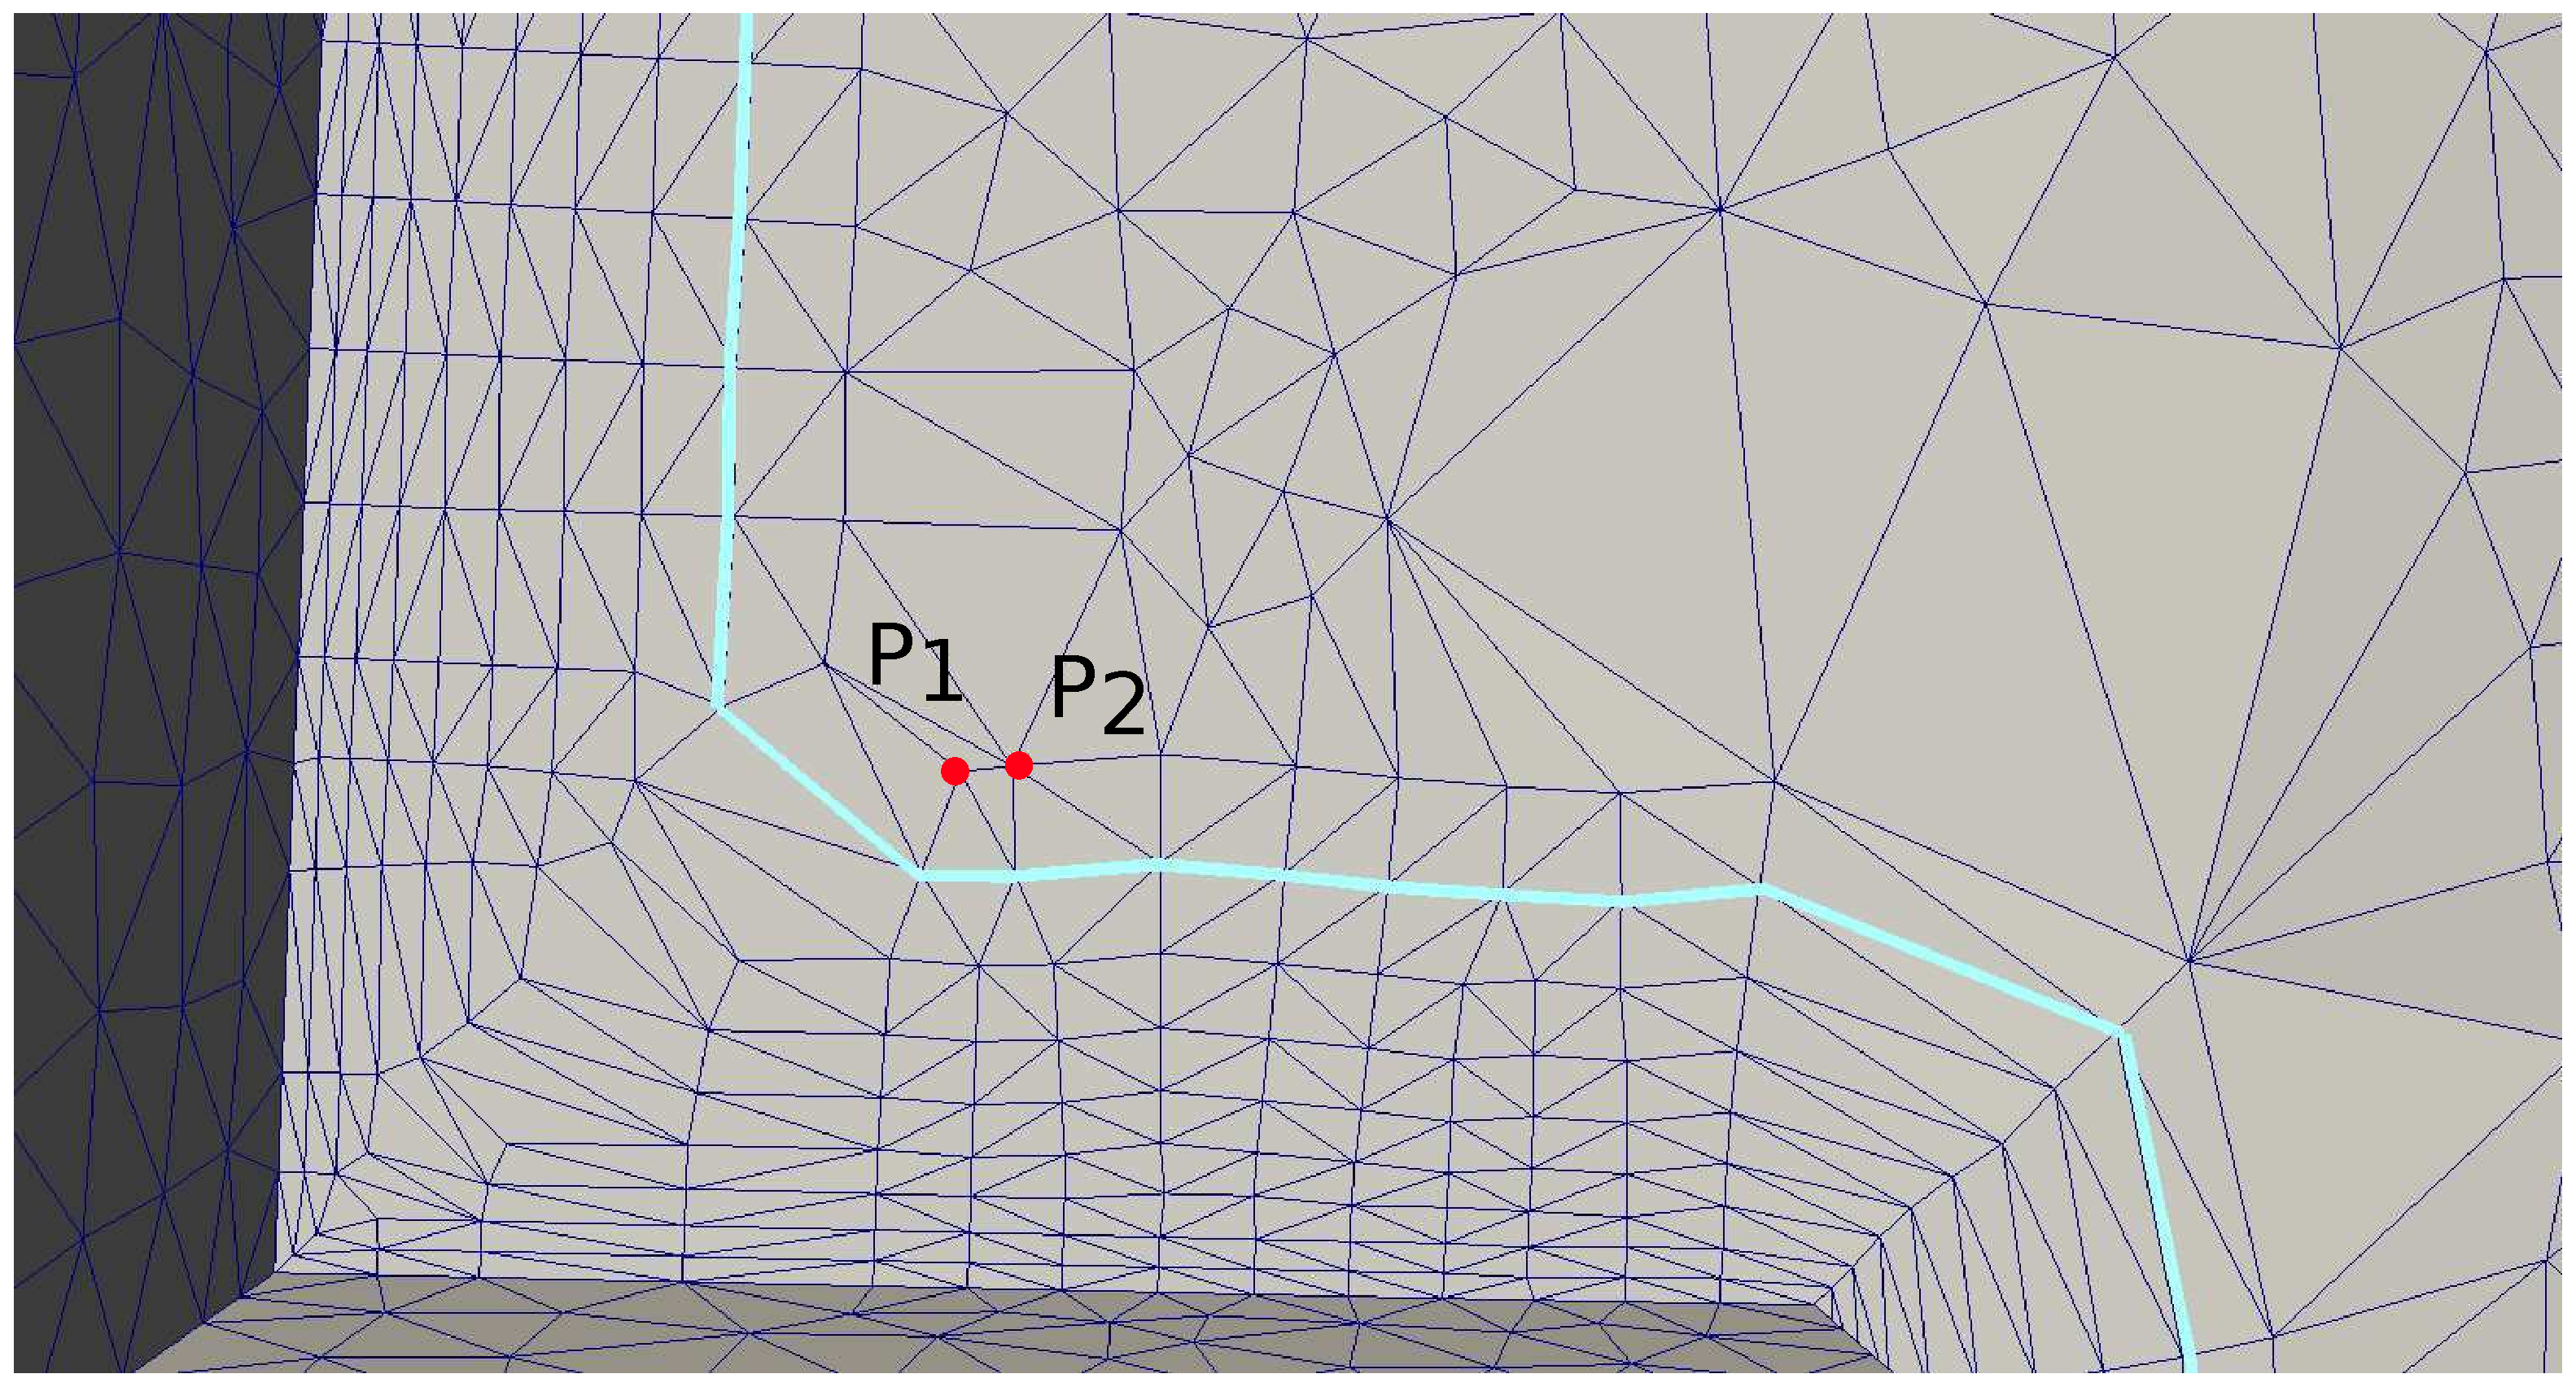
\includegraphics[width=.9\linewidth]{img/m2/edge-collapse/collapse1.eps}
  \caption{}
  \label{collapse1}
\end{subfigure}%
\begin{subfigure}{.5\textwidth}
  \centering
  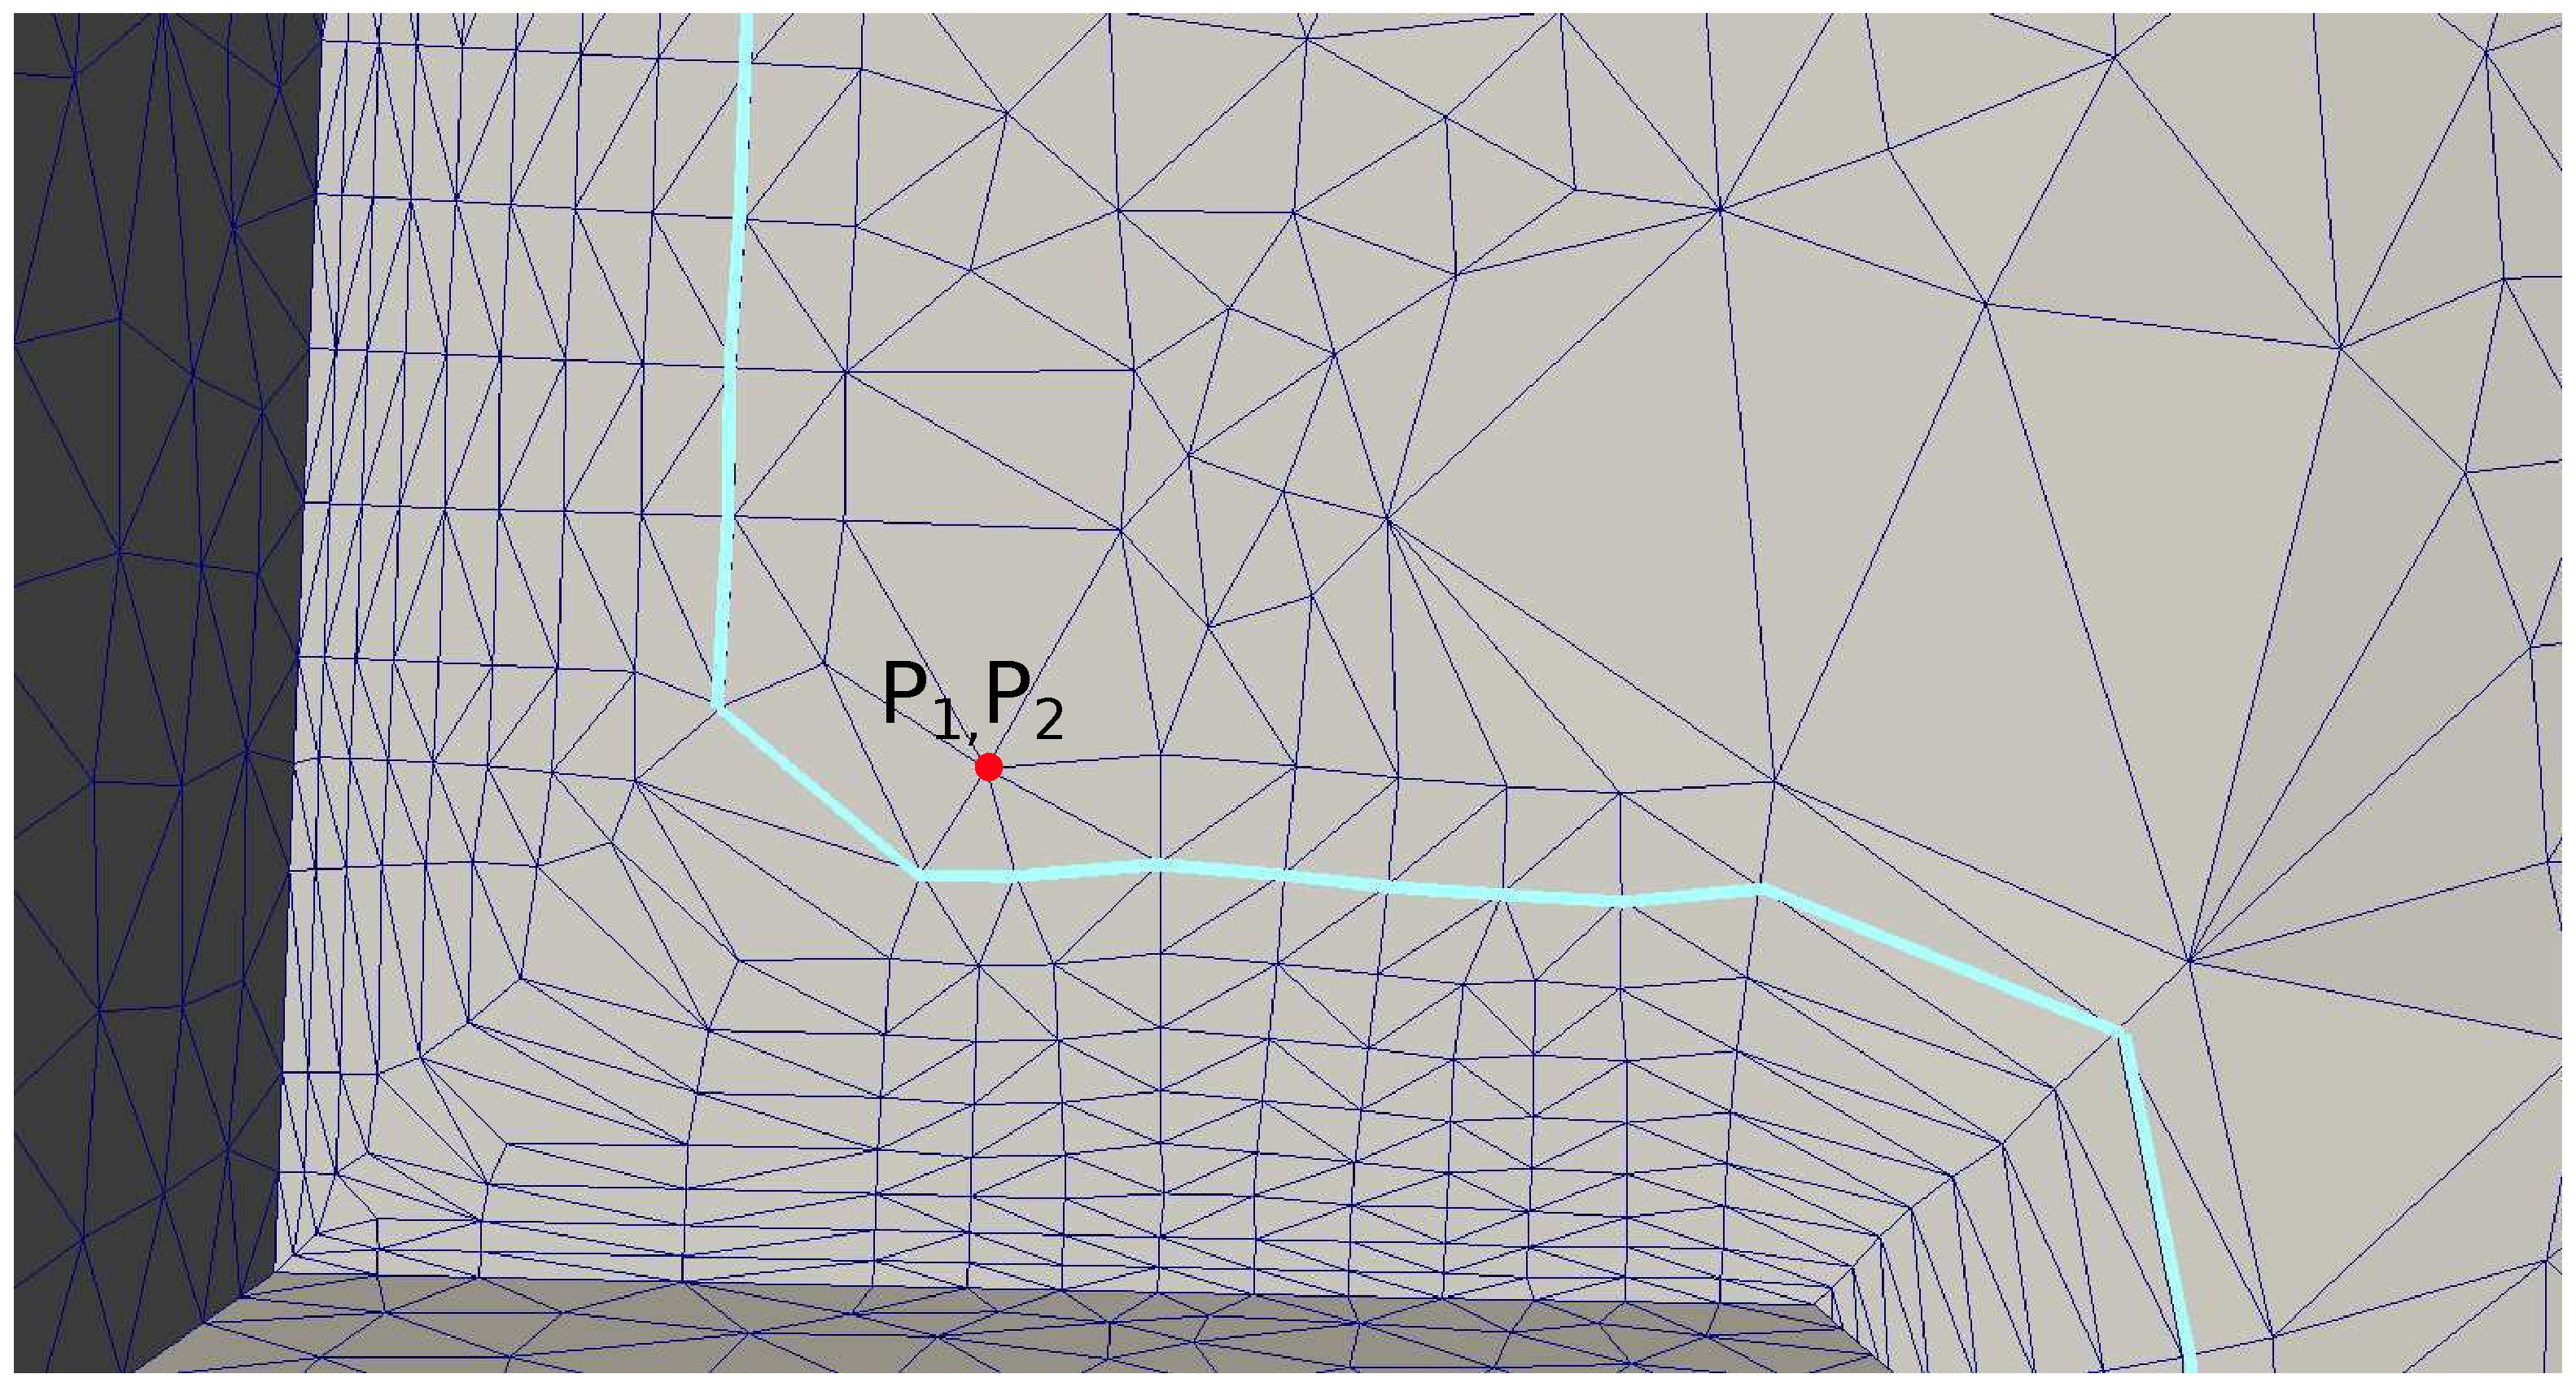
\includegraphics[width=.9\linewidth]{img/m2/edge-collapse/collapse2.eps}
  \caption{}
  \label{collapse2}
\end{subfigure}
\begin{subfigure}{.5\textwidth}
  \centering
  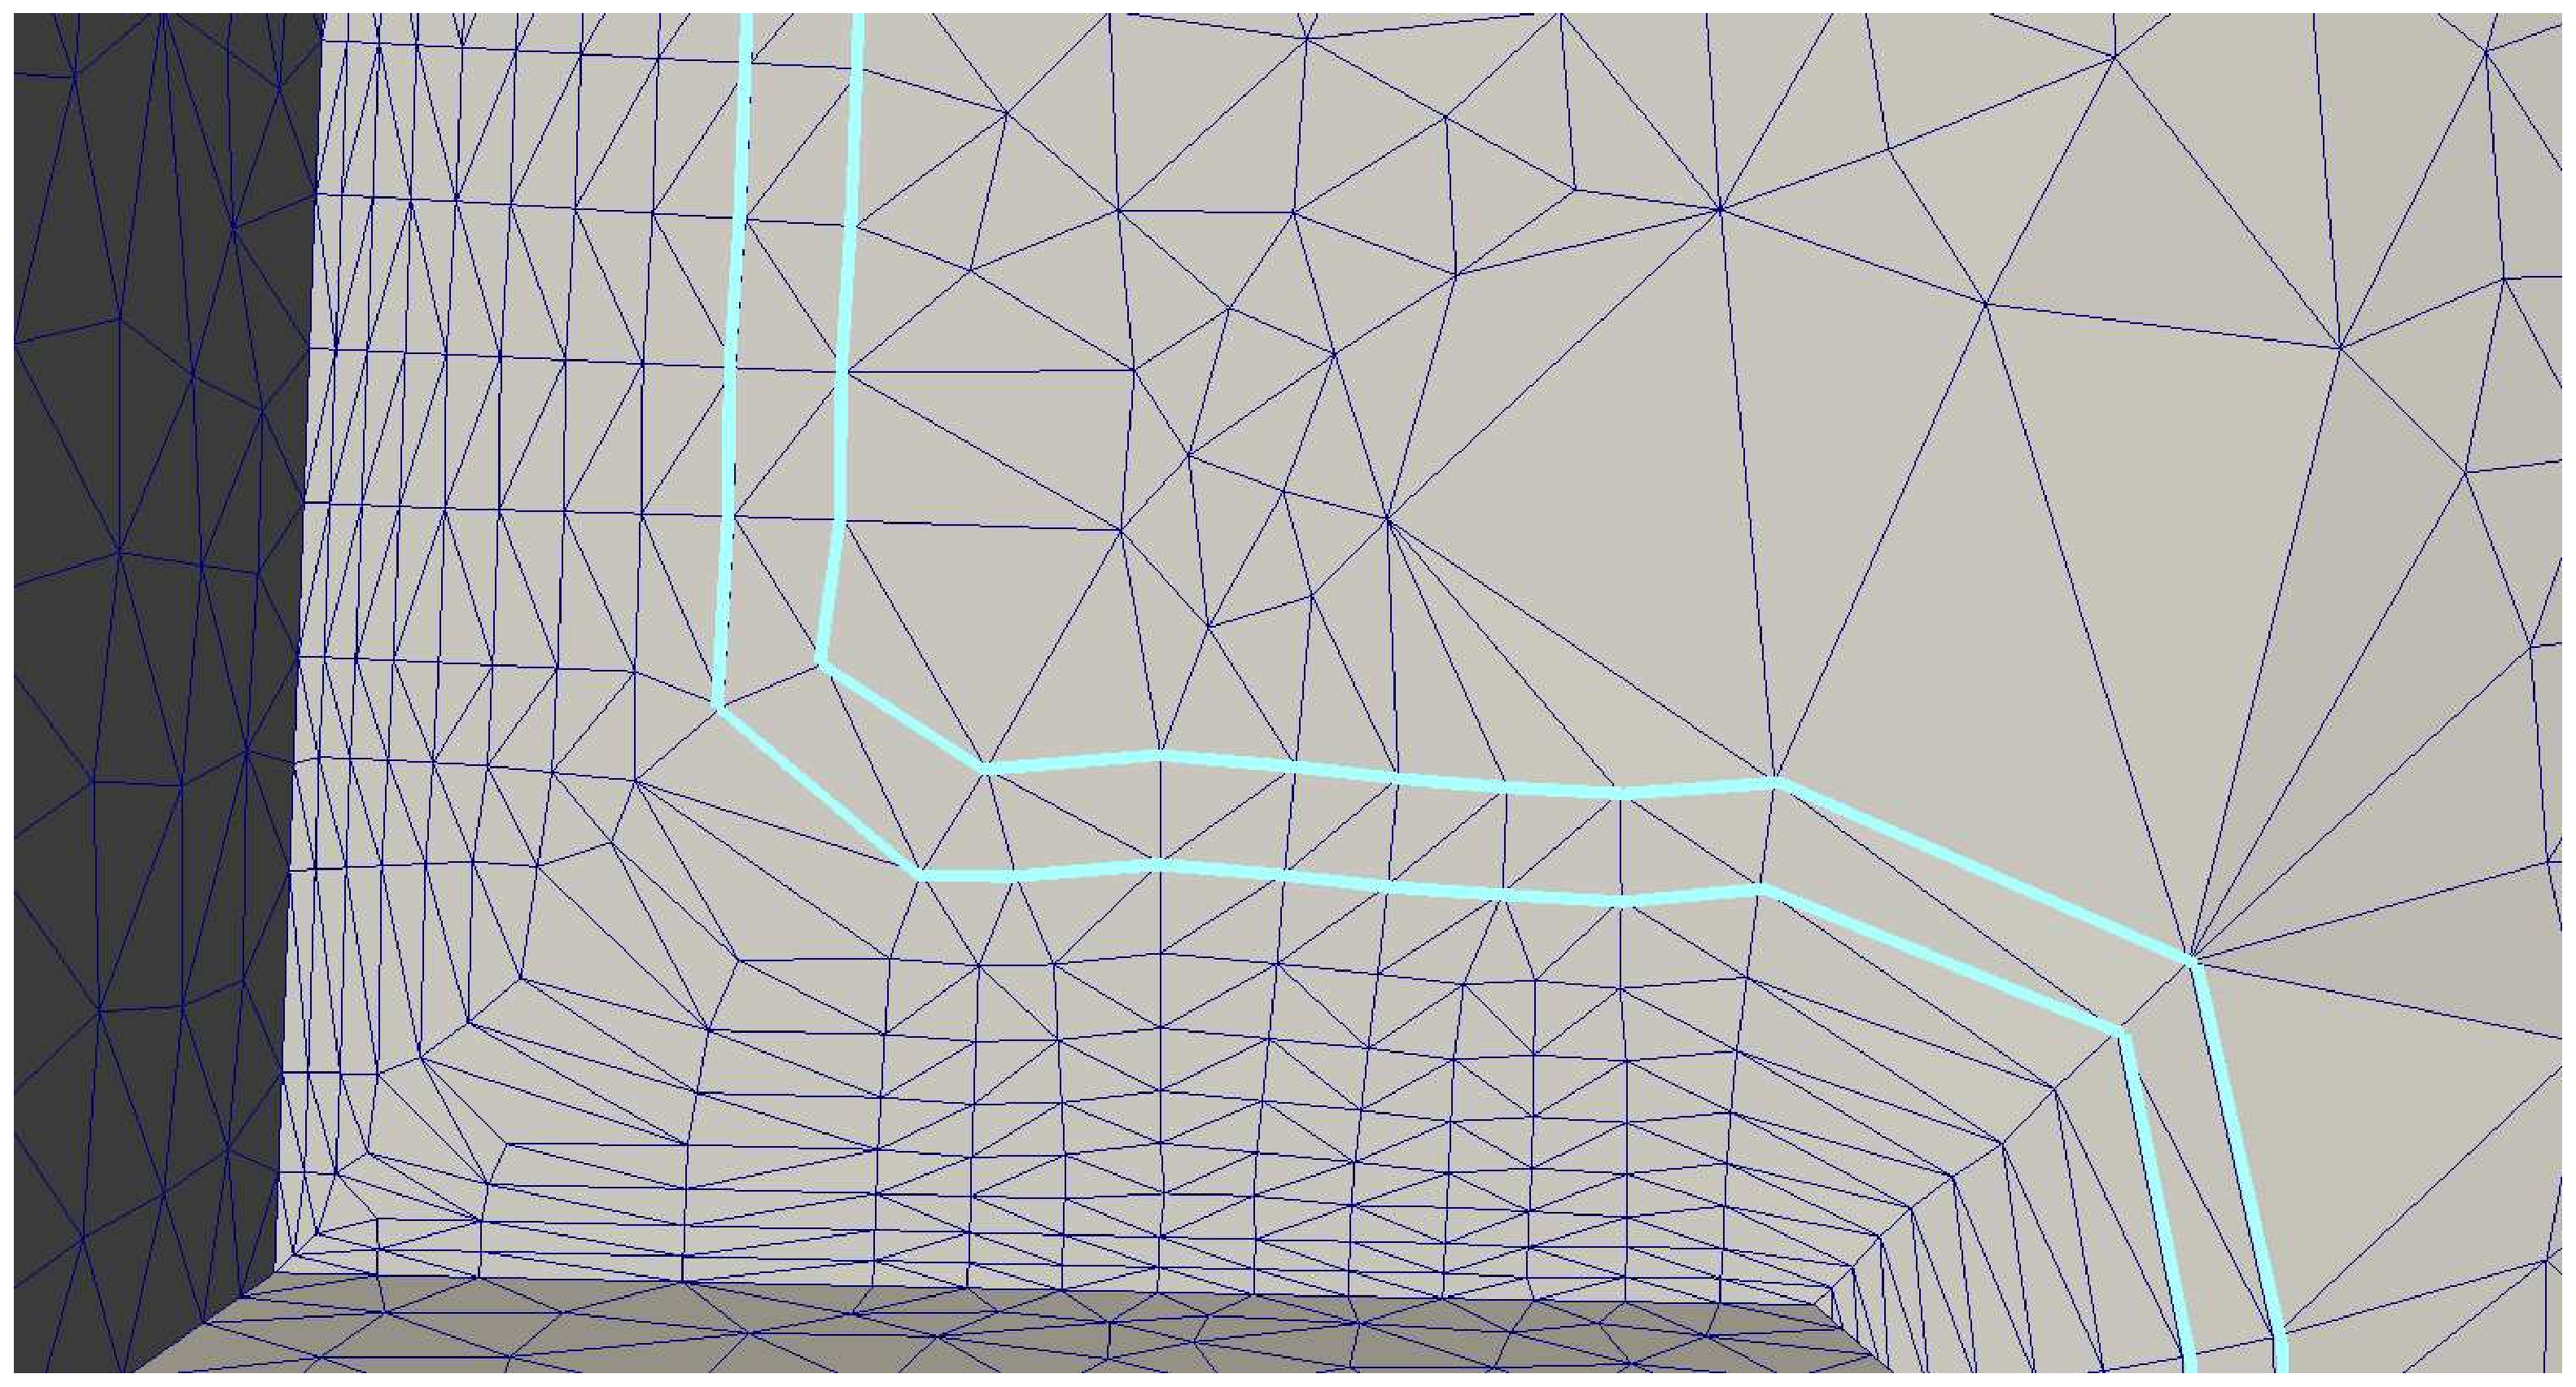
\includegraphics[width=.9\linewidth]{img/m2/edge-collapse/collapse3.eps}
  \caption{}
  \label{collapse3}
\end{subfigure}
\caption{Edge collapse on an advancing front to avoid encroachment of points. In (a), two points in the kid layer $P_1$ and $P_2$ are sufficiently close to each other. Their parent layer is highlighted. If both the points advance to the next layer, then the next front would fail to recover. Hence, the edge between them is chosen to collapse. (b) shows the result of the edge collapse. The new location of both the points is the average position of their initial location. (c) shows how the next front looks like.}
\label{edge-collapse}
\end{figure}

Once we have recovered the advancing front by iterative edge swaps to connect the kid points in the mesh, we check for vertices on the front that are too close to each other relative to the extrusion length. For instance, vertices which are near a concave corner could encroach each other if they are not decimated. Another example of a situation where vertex decimation on the advancing front becomes necessary is when the front has advanced to a substantial distance from the surface boundaries. In such a case, the extrusion length on the front has grown so much that the aspect ratio approaches unity. Decimating vertices from the front which are at a substantial distance from surface boundaries helps prevent the cell aspect ratio, ie front edge length over extrusion length, from dropping below one.

To check for vertices to decimate, we iterate through the vertices in the front and identify the ones which are too close to their neighbours. Vertex decimation is done through the edge-collapse routine as described in \cite{hoppe1994mesh}. The threshold edge length between two points on the front is set to be $2 \tan(\pi/8)$ times the average extrusion length at those points. This value is set so as to minimize the normalized maximum deviation of angle from $90^\circ$ for quad elements. Hence, the threshold ensures that the anisotropic properties are retained for several layers into the surface. All short edges on the front are collapsed using the edge-collapse algorithm. An example of an edge-collapse on the front is shown in Figure \ref{edge-collapse}. Here, two points $P_1$ and $P_2$ are collapsed into a single point which forms a part of the next front on the surface. Mathematically,

\begin{equation}
l_{\mathit{collapse}} = 2 \cdot \; tan \left( \frac{pi}{8} \right) \cdot \; x_n \; ;
\end{equation}

where $l_{\mathit{collapse}}$ is the minimum length of an edge on the advancing front which will not be considered for edge collapse and $x_n$ is the extrusion length at the $n^{th}$ layer.

%Validation checks are made before collapsing an edge. The deviation of the triangles formed as a result of edge collapse from the underlying surface is constrained to be less than $30^{\circ}$ to limit the deviation of the mesh from the ground truth surface $S$. 

Topological and geometrical checks are done before an edge can be collapsed in the mesh. These include a threshold for the ratio of area of generated triangles and a limit on the dihedral angle between the adjacent triangles created by the collapse. The area threshold is set to be $10^8$. Also, edge-collapse is successful only if the triangles resulting from it are be within a limit of $\theta < 30^{\circ}$ from the surface(see Figure \ref{deviation-surface}). The threshold for the maximum dihedral angle between any two adjacent triangles that result from the edge-collapse is set to $40^{\circ}$. 

After we have a recovered the front and decimated encroaching vertices in the surface interior as well as on the advancing front through edge collapse, we queue up the immediate interior edges of the surface and swap them for maximizing mesh quality. This step is included so that we have a good interior triangulation at each step of the advancing layer routine. This step ensures that we do not have bad triangles causing problems as we continue to march.

The edge collapse subroutine on the advancing front helps in controlling the aspect ratio at the front and limit its minimum value to 1. Once the aspect ratio has approached a value of $1$ on the front, layers will continue to extrude without growth in their size. Additionally, at concave corners with low aspect ratios, the edge collapse subroutine helps in maintaining a valid front to continue marching towards surface interior.

\subsection{Vertex Decimation in Sub-Surface Interior}

As discussed in the previous chapter, we follow a closed advancing front methodology to generate the anisotropic surface mesh. The input triangulation $T$, which is the encoding of the surface $S$ is taken to be the initial mesh. Such a technique helps us in maintaining a complete and valid surface mesh at each step in the mesh generation process. However, this means that we need to do some additional work in deleting the vertices on the sub-surface imported initially which are no longer required to be a part of the anisotropic surface mesh. Fortunately, we have all the connectivity information of the vertices on the front. This means that we do not have to scan the 3D space near the vertex to find the encroaching points. Checking the vertices in surface interior which share an edge with the front vertex is sufficient.

\begin{figure}[hbt!]
\centering
\begin{subfigure}{.5\textwidth}
  \centering
  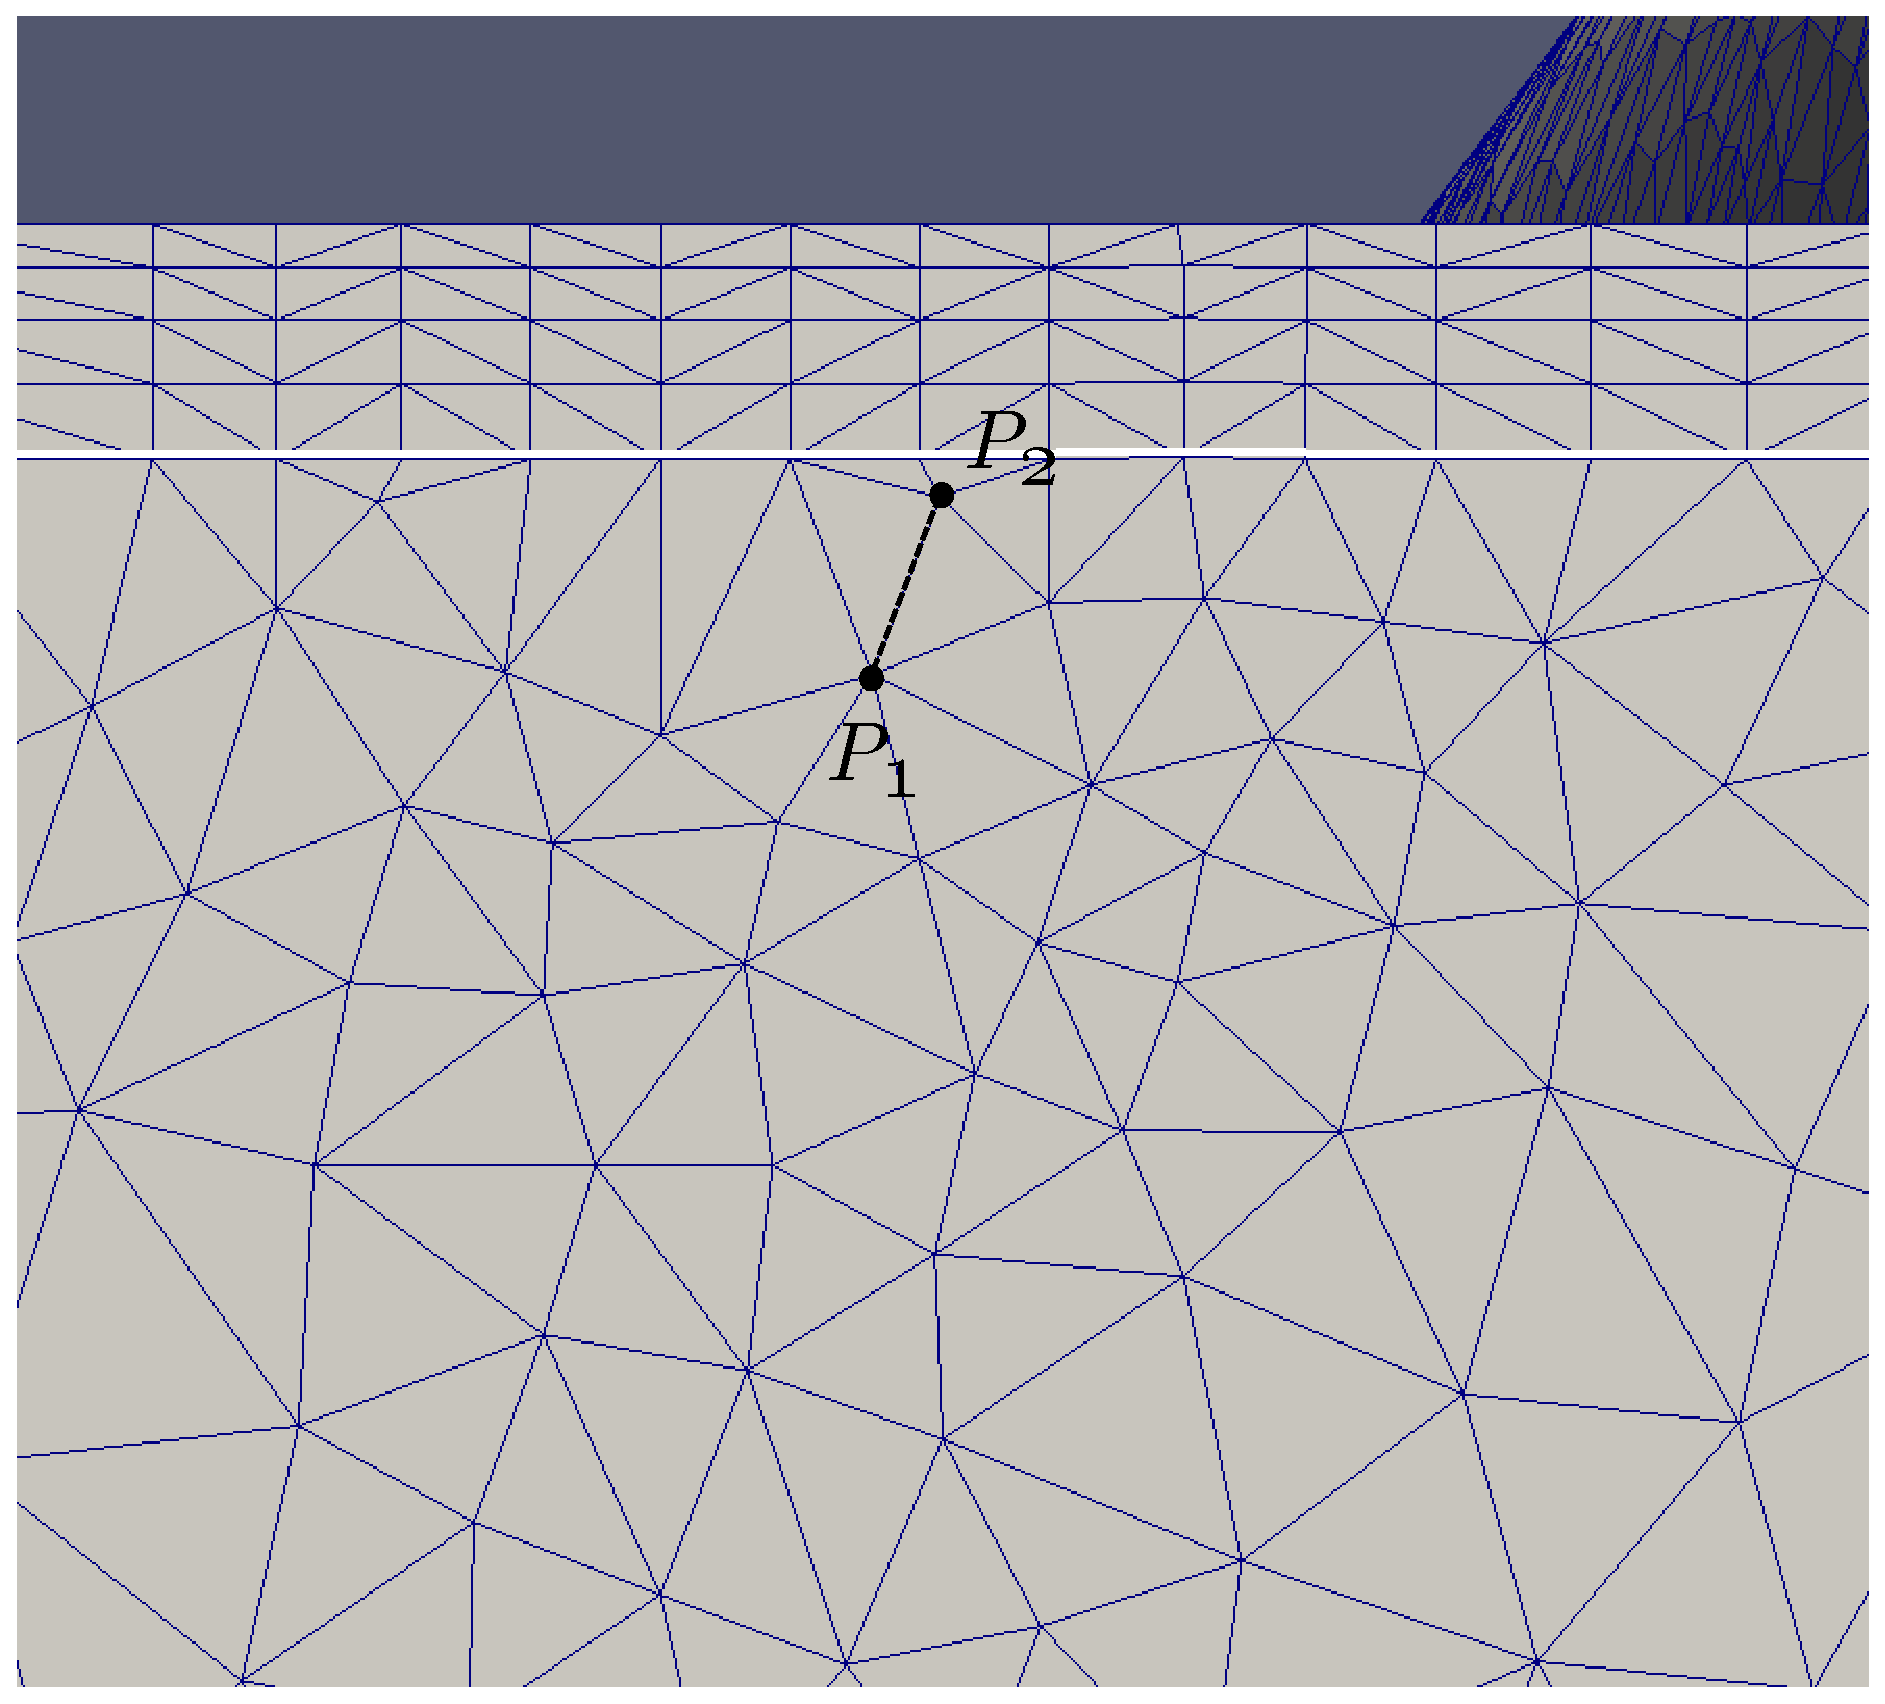
\includegraphics[width=.9\linewidth, trim={0 5cm 0  0}, clip]{img/m2/interior-vert-collapse/cc1.eps}
  \caption{}
  \label{cc1}
\end{subfigure}%
\begin{subfigure}{.5\textwidth}
  \centering
  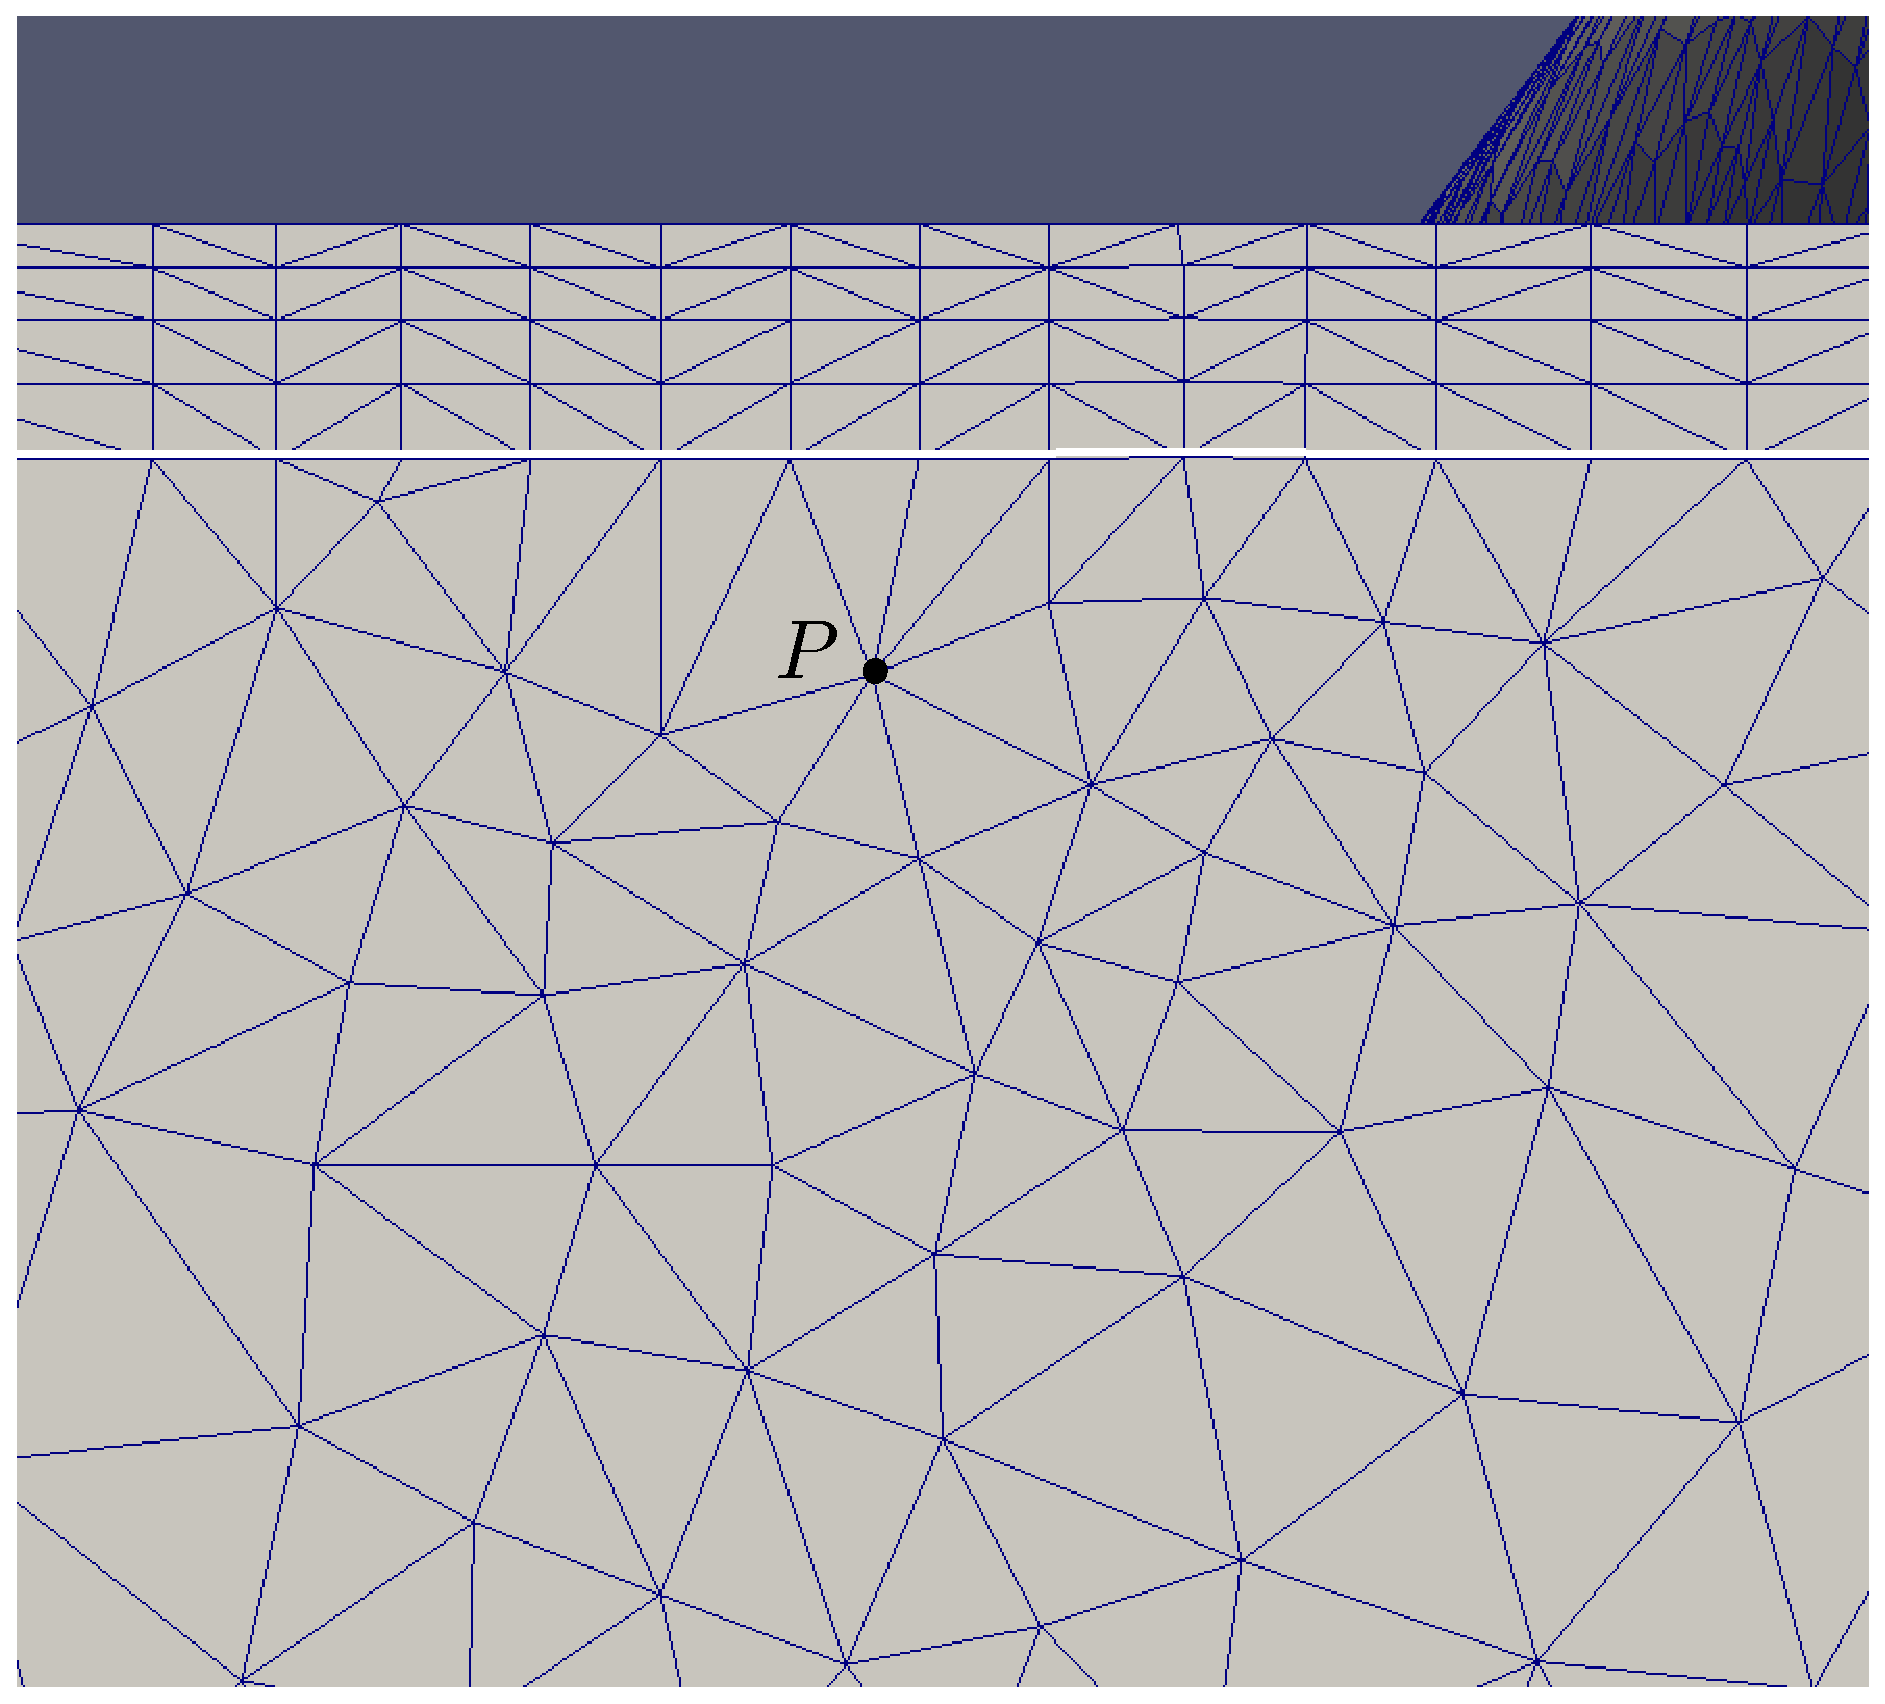
\includegraphics[width=.9\linewidth, trim={0 5cm 0  0}, clip]{img/m2/interior-vert-collapse/cc2.eps}
  \caption{}
  \label{cc2}
\end{subfigure}
\begin{subfigure}{.5\textwidth}
  \centering
  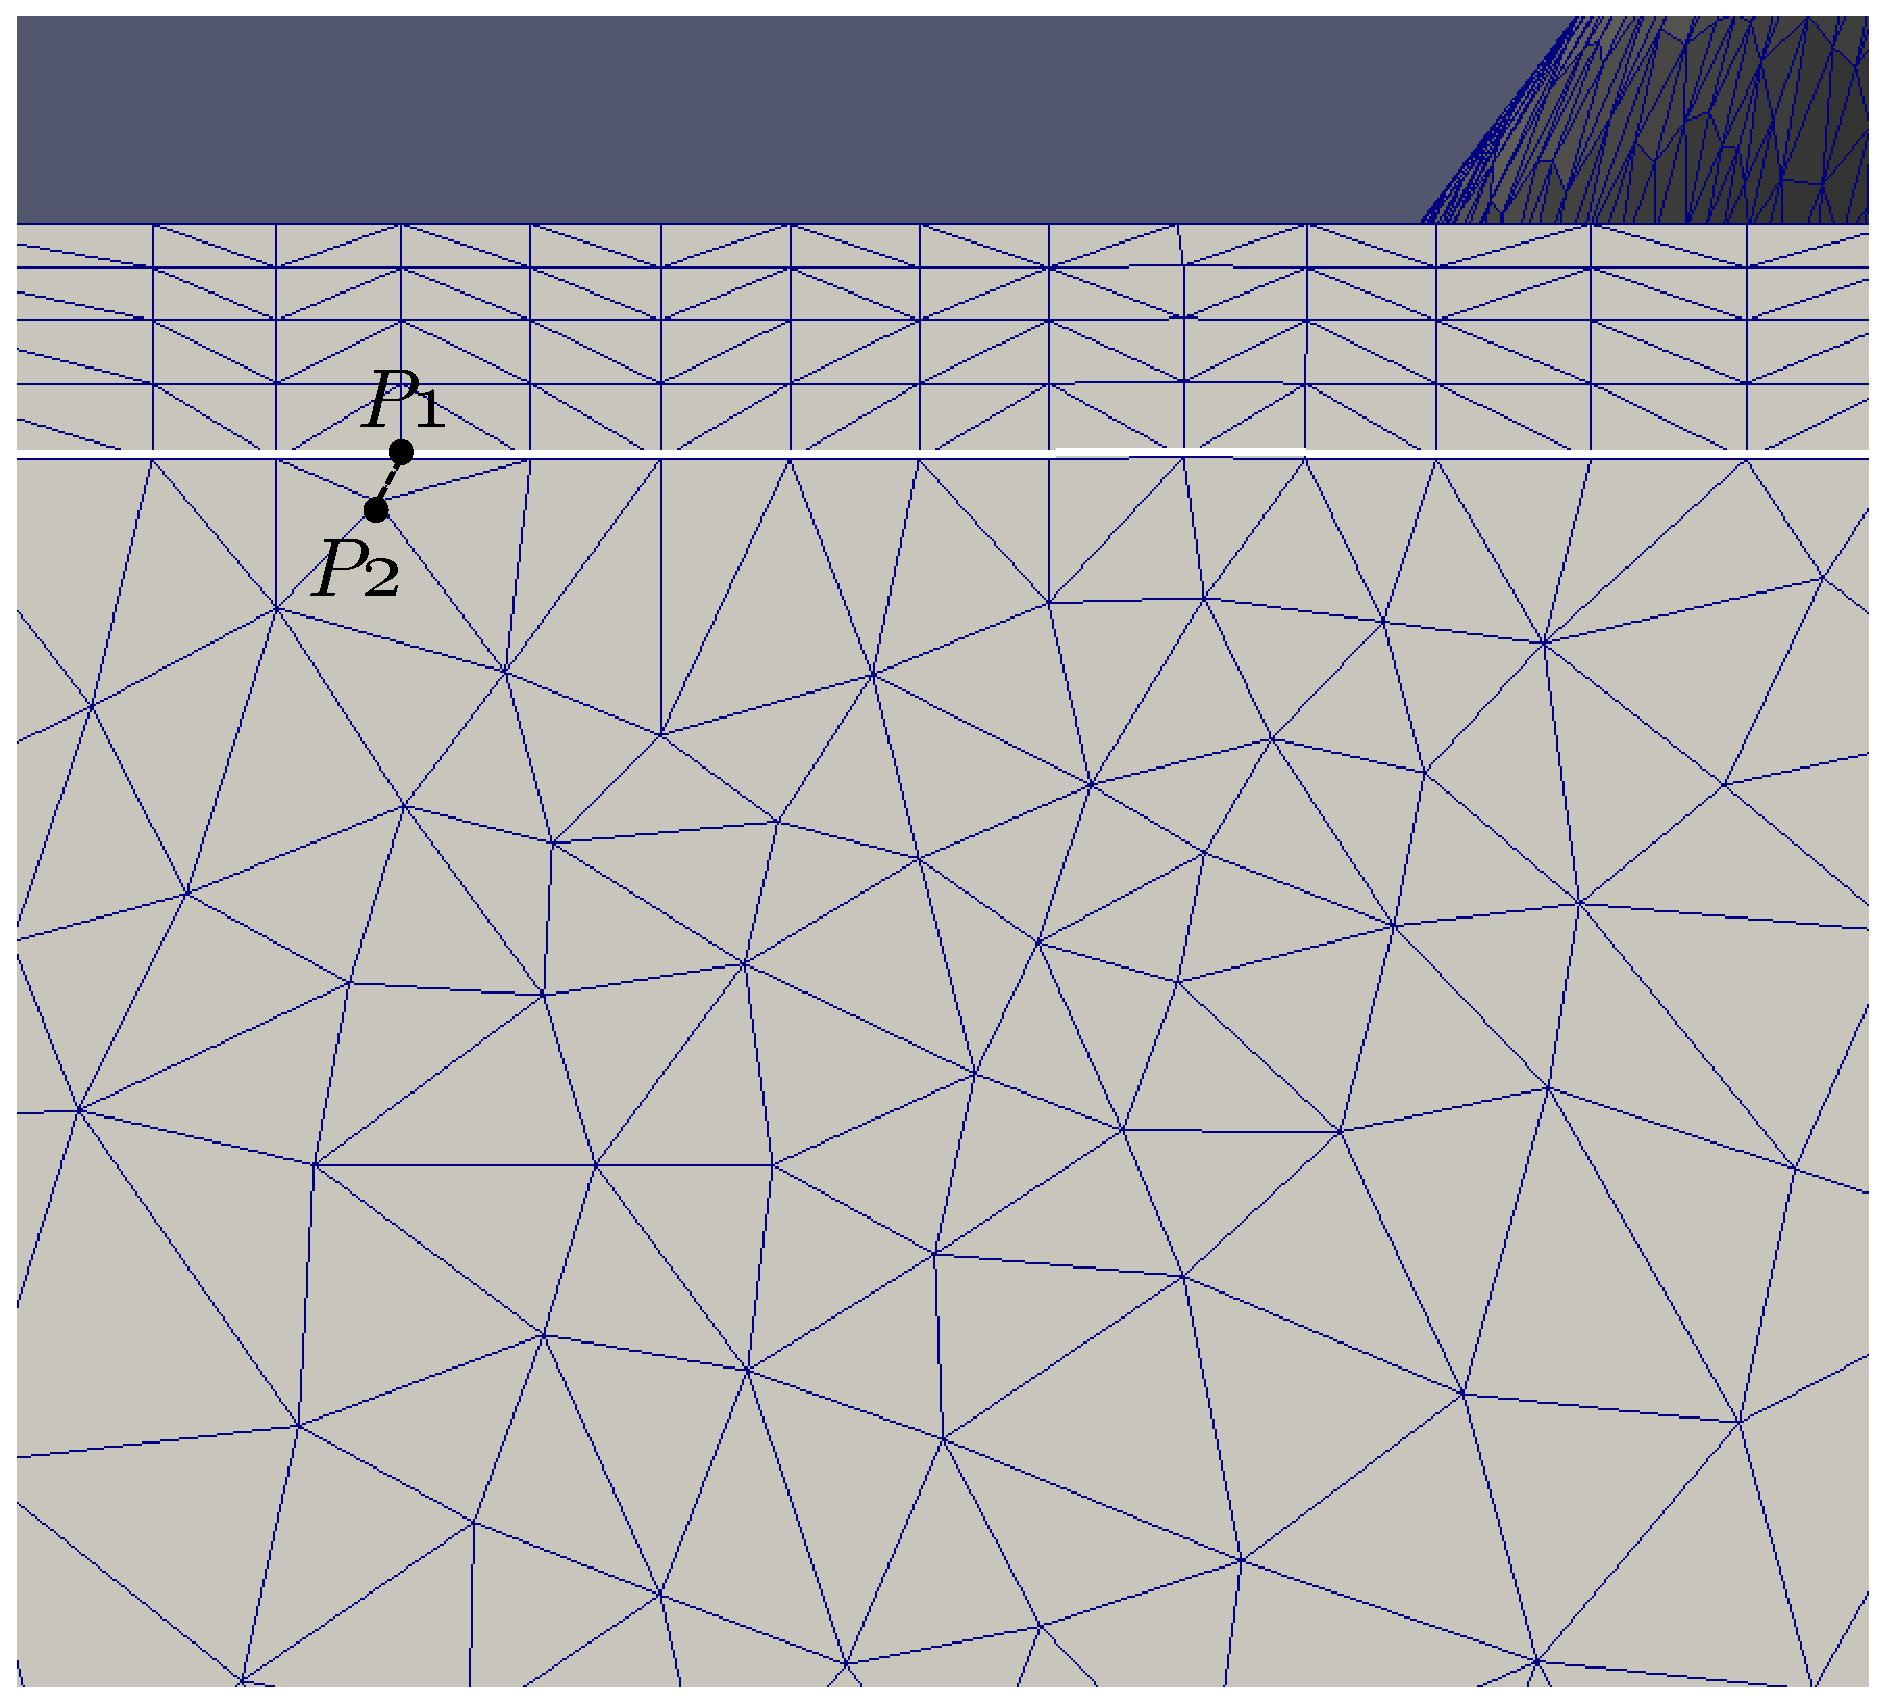
\includegraphics[width=.9\linewidth, trim={0 5cm 0  0}, clip]{img/m2/interior-vert-collapse/cc3.eps}
  \caption{}
  \label{cc3}
\end{subfigure}%
\begin{subfigure}{.5\textwidth}
  \centering
  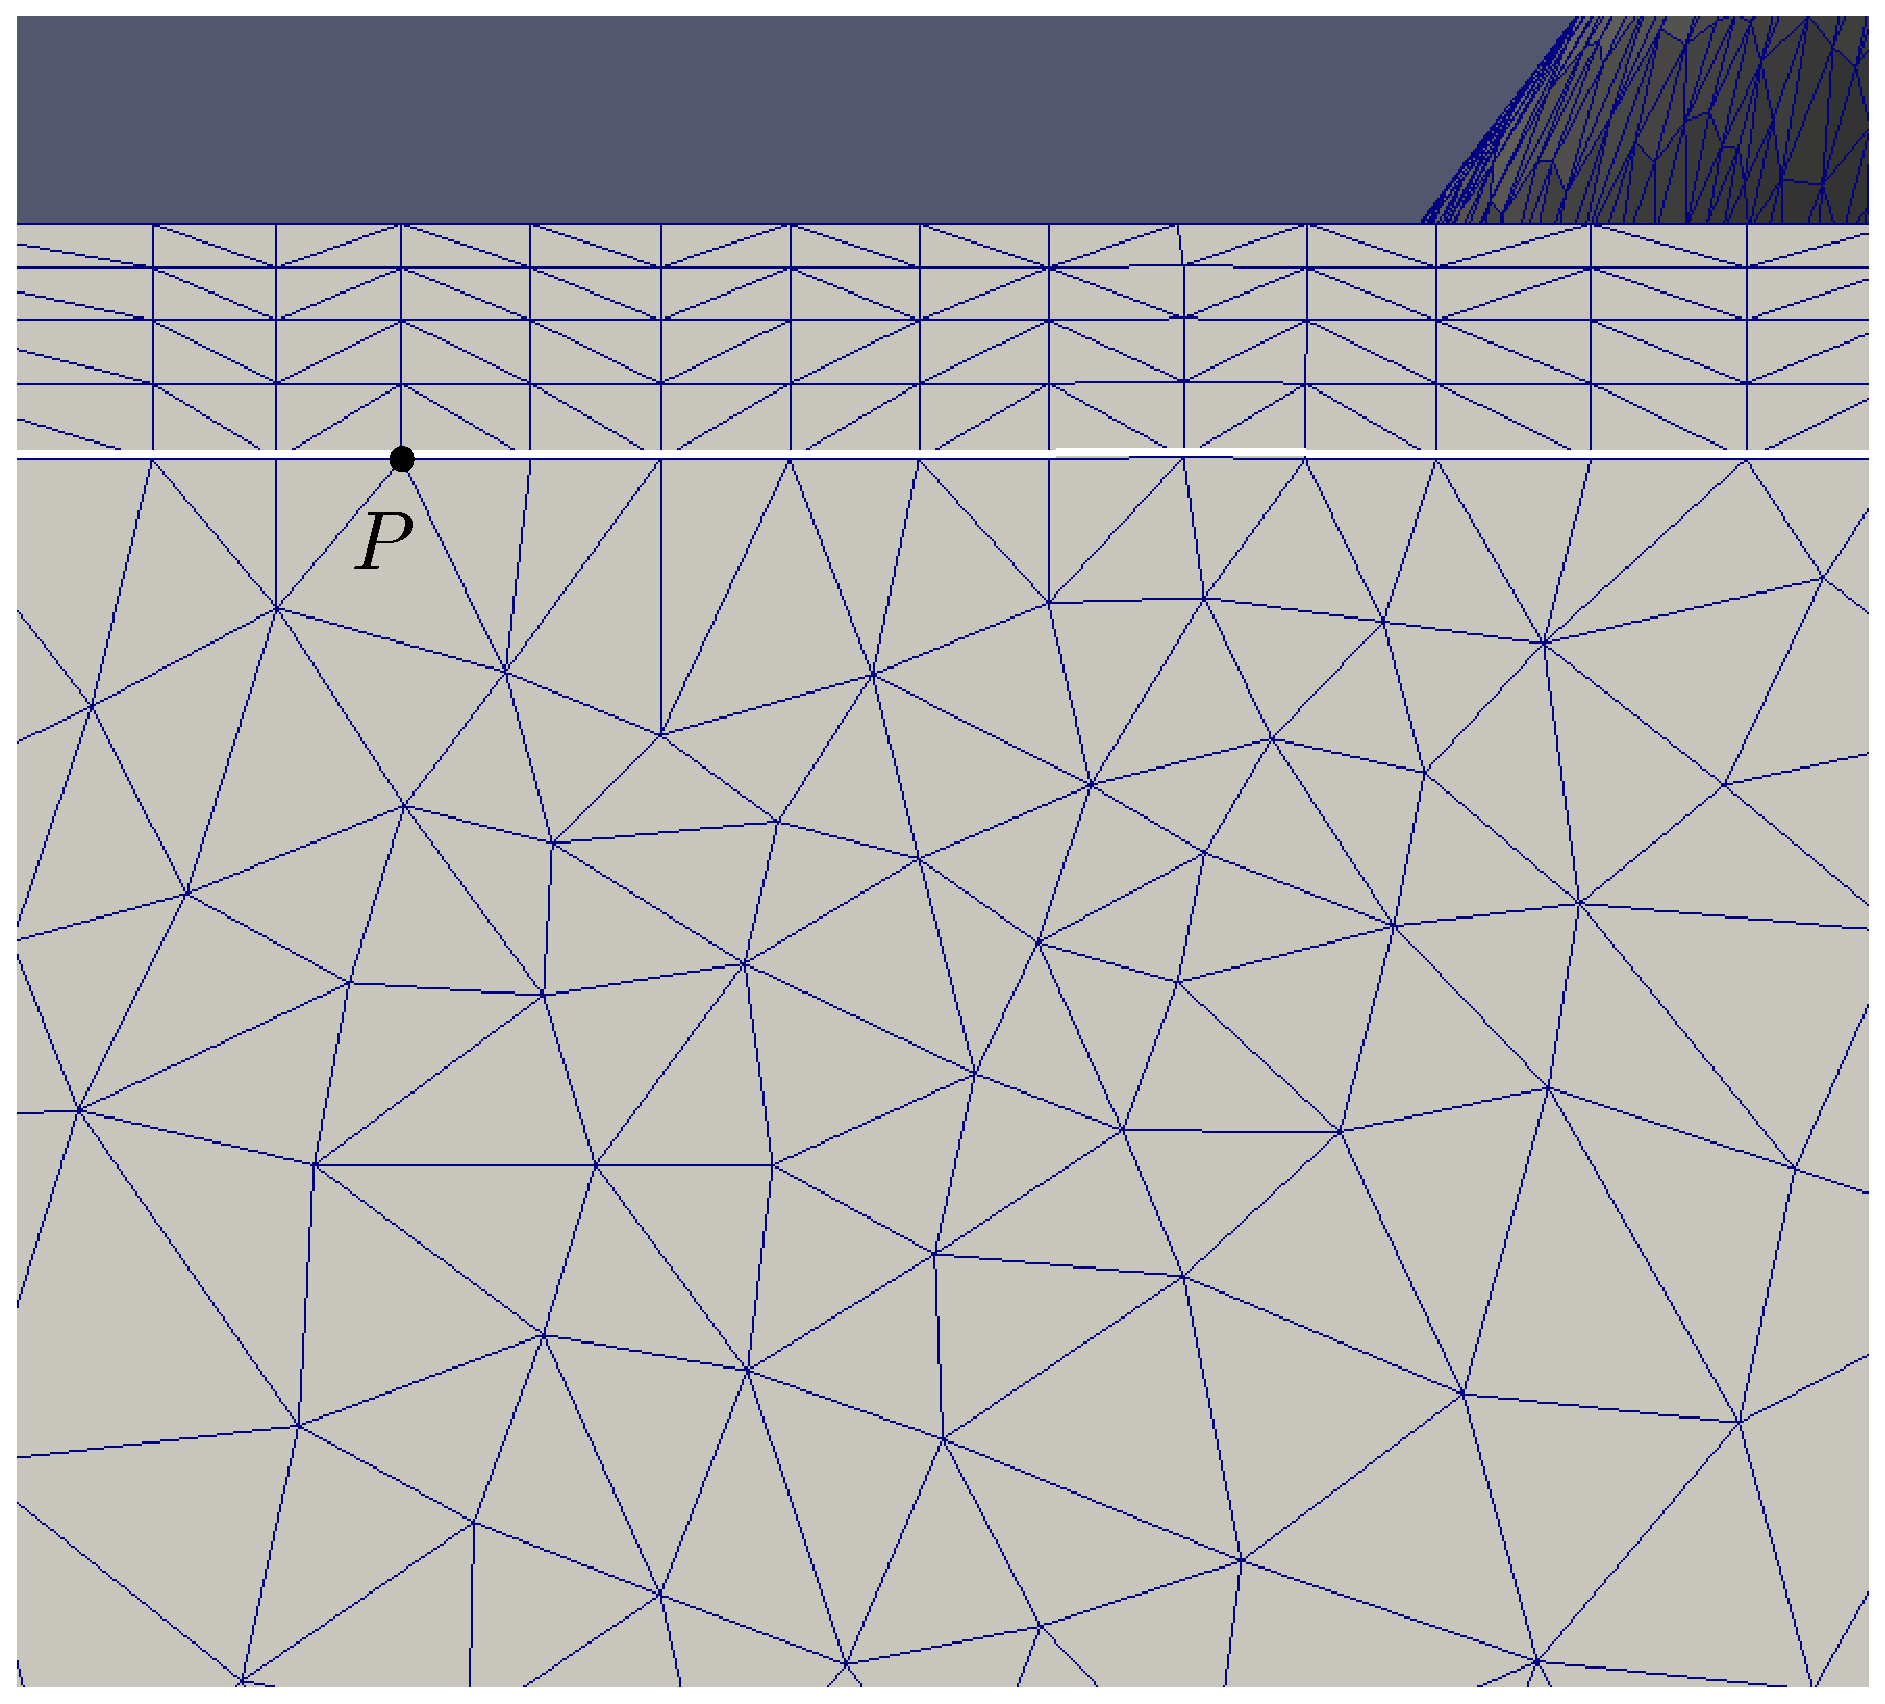
\includegraphics[width=.9\linewidth, trim={0 5cm 0  0}, clip]{img/m2/interior-vert-collapse/cc4.eps}
  \caption{}
  \label{cc4}
\end{subfigure}
\caption{Interior vertex decimation through edge collapse. The highlighted white line shows the advancing front. In (a), vertex $P_2$ is about to encroach the front. Hence, the best vertex for collapse is chosen among its neighbours. The best vertex for edge collapse here is $P_1$. Hence, $P_2$ is collapsed on to $P_1$. The connectivity after the edge collapse is shown in (b) where vertex $P$ represents the collapsed vertex. Similarly, in (c), vertex $P_2$ is about to encroach the advancing front and is collapsed onto vertex $P_1$ which is on the advancing front itself. The new connectivity is shown in (d) where all the possibly encroaching vertices for the advancing layer are decimated.}
\label{interior-vert-collapse}
\end{figure}

In other words, as the advancing front marches into the surface, vertices in the interior of the surface immediately next to the front are decimated to make way for the advancing layers. Before extruding a point $P$ on the advancing front, we check if any point in the surface interior with which it shares an edge agrees with the following condition. If it does, we decimate the interior vertex.

\begin{equation}
    d < max \left( \frac{l_{1}}{\sqrt{2}}, \, \frac{l_{2}}{\sqrt{2}}, \; c \cdot  \mathit{x_n}\right)
    \label{collapse-eq}
\end{equation}

Here $d$ is the distance between the point on the advancing front and the interior point, $l_1$ and $l_2$ are the lengths of adjacent front edges of the point on the front, c is a constant whose value is set as $2$ and $x_n$ is the extrusion length at the vertex on the $n^{th}$ front. This condition ensures decimation of vertices in the surface interior which are close to the advancing front and avoids any encroachment of surface interior vertices on the advancing layers. 

Validation checks for front edge collapse mentioned in the last subsection are also run during interior edge collapse. The quality criterion used for interior edge collapse is maximization of the minimum angle in the triangles thus produced. The best edge for collapse is chosen when decimating the interior vertices using this quality criterion. This is in contrast to the vertex decimation on the advancing front where the candidate edge for collapse is already identified. An illustrative example for surface interior vertex decimation can be seen in Figure \ref{interior-vert-collapse}.

\section{Combining Triangular Elements to Quadrilateral Elements}

In section \ref{sec-simplicial}, we discussed about the pros and cons of simplical and non-simplical mesh elements. Then, in section \ref{consolidate-motivation}, we talked about the motivation to produce a hybrid surface mesh which consists of both simplical and non-simplical mesh elements. Briefly, a hybrid anisotropic surface mesh which consists primarily of quadrilateral elements with a small number of triangular elements gives us the flexibility to mesh topologically complex surface geometries while keeping the average vertex connectivity of the mesh to a low value.

Almost all vertices in our closed advancing front method have a parent-kid relationship. The successor of a vertex is called its kid while the predecessor is called the parent. There are a couple of exceptions to this. First, vertices on the boundary curve do not have a parent as they are the zeroth layer of the mesh. Second, wherever an edge collapse operation is done, two kids from two different parent vertices collapse into a single vertex. This leaves a kid vertex with two parents, or, in other words, a two parents who share a common kid vertex.

\vspace{10pt}
\begin{figure}[hbt!]
\centering
\begin{subfigure}{\textwidth}
  \centering
  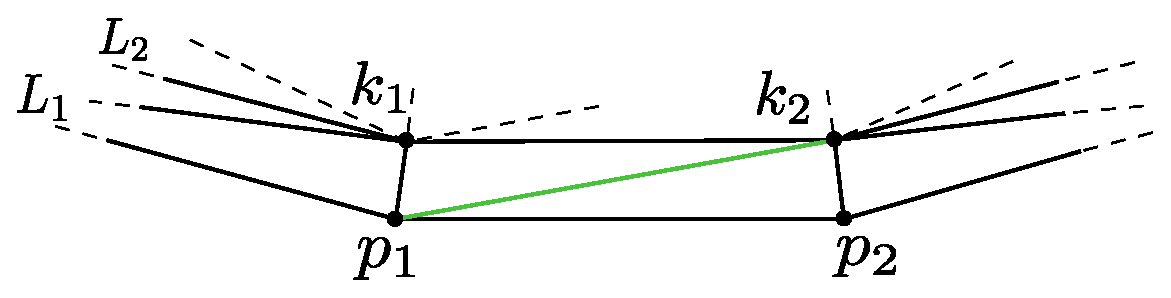
\includegraphics[width=.7\linewidth]{img/m2/combineTriToQuad.eps}
  \caption{}
  \label{triToQuad1}
\end{subfigure}
\begin{subfigure}{\textwidth}
  \centering
  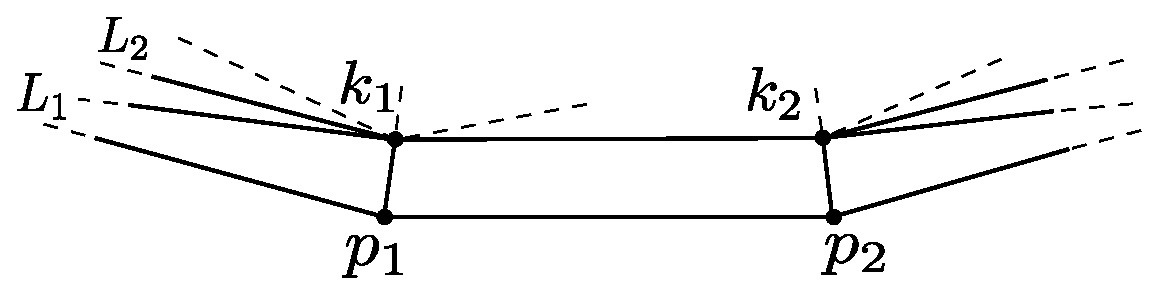
\includegraphics[width=.7\linewidth]{img/m2/combineTriToQuad2.eps}
  \caption{}
  \label{triToQuad2}
\end{subfigure}
\caption{}
\label{triToQuad}
\end{figure}

Apart from the two exceptions just mentioned, all the vertices have a parent and a kid. This gives some structure to our mesh. As the layers grow in the normal direction to the boundary curve, this helps us in generating rectangular quadrilateral elements easily. Edges are removed from the finished layers so as to generate superior quality quadrilateral cells. As the layers advance from the boundary curves towards the tangential direction onto the surface, the quadrilateral elements generated retain the boundary topology several layers into the interior of the surface. The quality of a quadrilateral element is calculated as the inverse of the maximum deviation of its interior angles from 90 degrees. This criterion is selected so as to prefer rectangular elements and retain the boundary representation on the surface mesh. Starting from the first layer generated on the surface, multiple iterations of this subroutine are run for the same layer to ensure as few triangular elements are left per layer as possible.

Consider Figure \ref{triToQuad1}. $L_1$ and $L_2$ denote two successive layers on the advancing layer mesh. Points $p_1$ and $p_2$ are on the parent layer $L_1$ and their kids, $k_1$ and $k_2$, respectively, are on the kid layer $L_2$. All the edges in the neighbourhood of $p_1$ and $p_2$ which are not on the advancing front are queued. Then, these edges are sorted in order of the quality of the quadrilateral elements generated after their removal. Finally, all the edges in the queue are deleted until both the elements which share the edge are triangular. The edged marked in green color in the figure is deleted in the process which results in the deletion of two triangular elements and generation of a new quadrilateral element. The local mesh after edge removal is shown in Figure \ref{triToQuad2}.

\vspace{10pt}
\begin{figure}[hbt!]
  \centering
  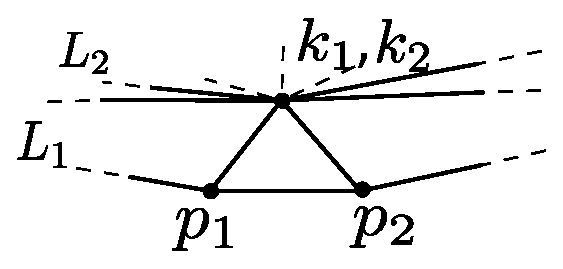
\includegraphics[width=0.5\linewidth]{img/m2/combineTriToQuad3.eps}
  \caption{•}
  \label{triLeft}
\end{figure}

As discussed earlier, some exceptions exist in the advancing layer mesh where all the elements in a layer cannot be converted to a quadrilateral element. An illustration of such an exception is shown in Figure \ref{triLeft}. Here, two kids $k_1$ and $k_2$ had to collapse to a single vertex as the edge between them is collapsed in the aspect ratio control subroutine explained in section \ref{aspectRatioControl}. Hence, a triangle would be left in between layers $L_1$ and $L_22$. An example surface mesh which shows the result of the combine triangular elements to quadrilateral elements subroutine can be seen in Figure \ref{fig-triQuad}. Most of the triangular mesh elements are converted to quadrilateral elements save a few.

\begin{figure}
\centering
\begin{subfigure}{0.5\textwidth}
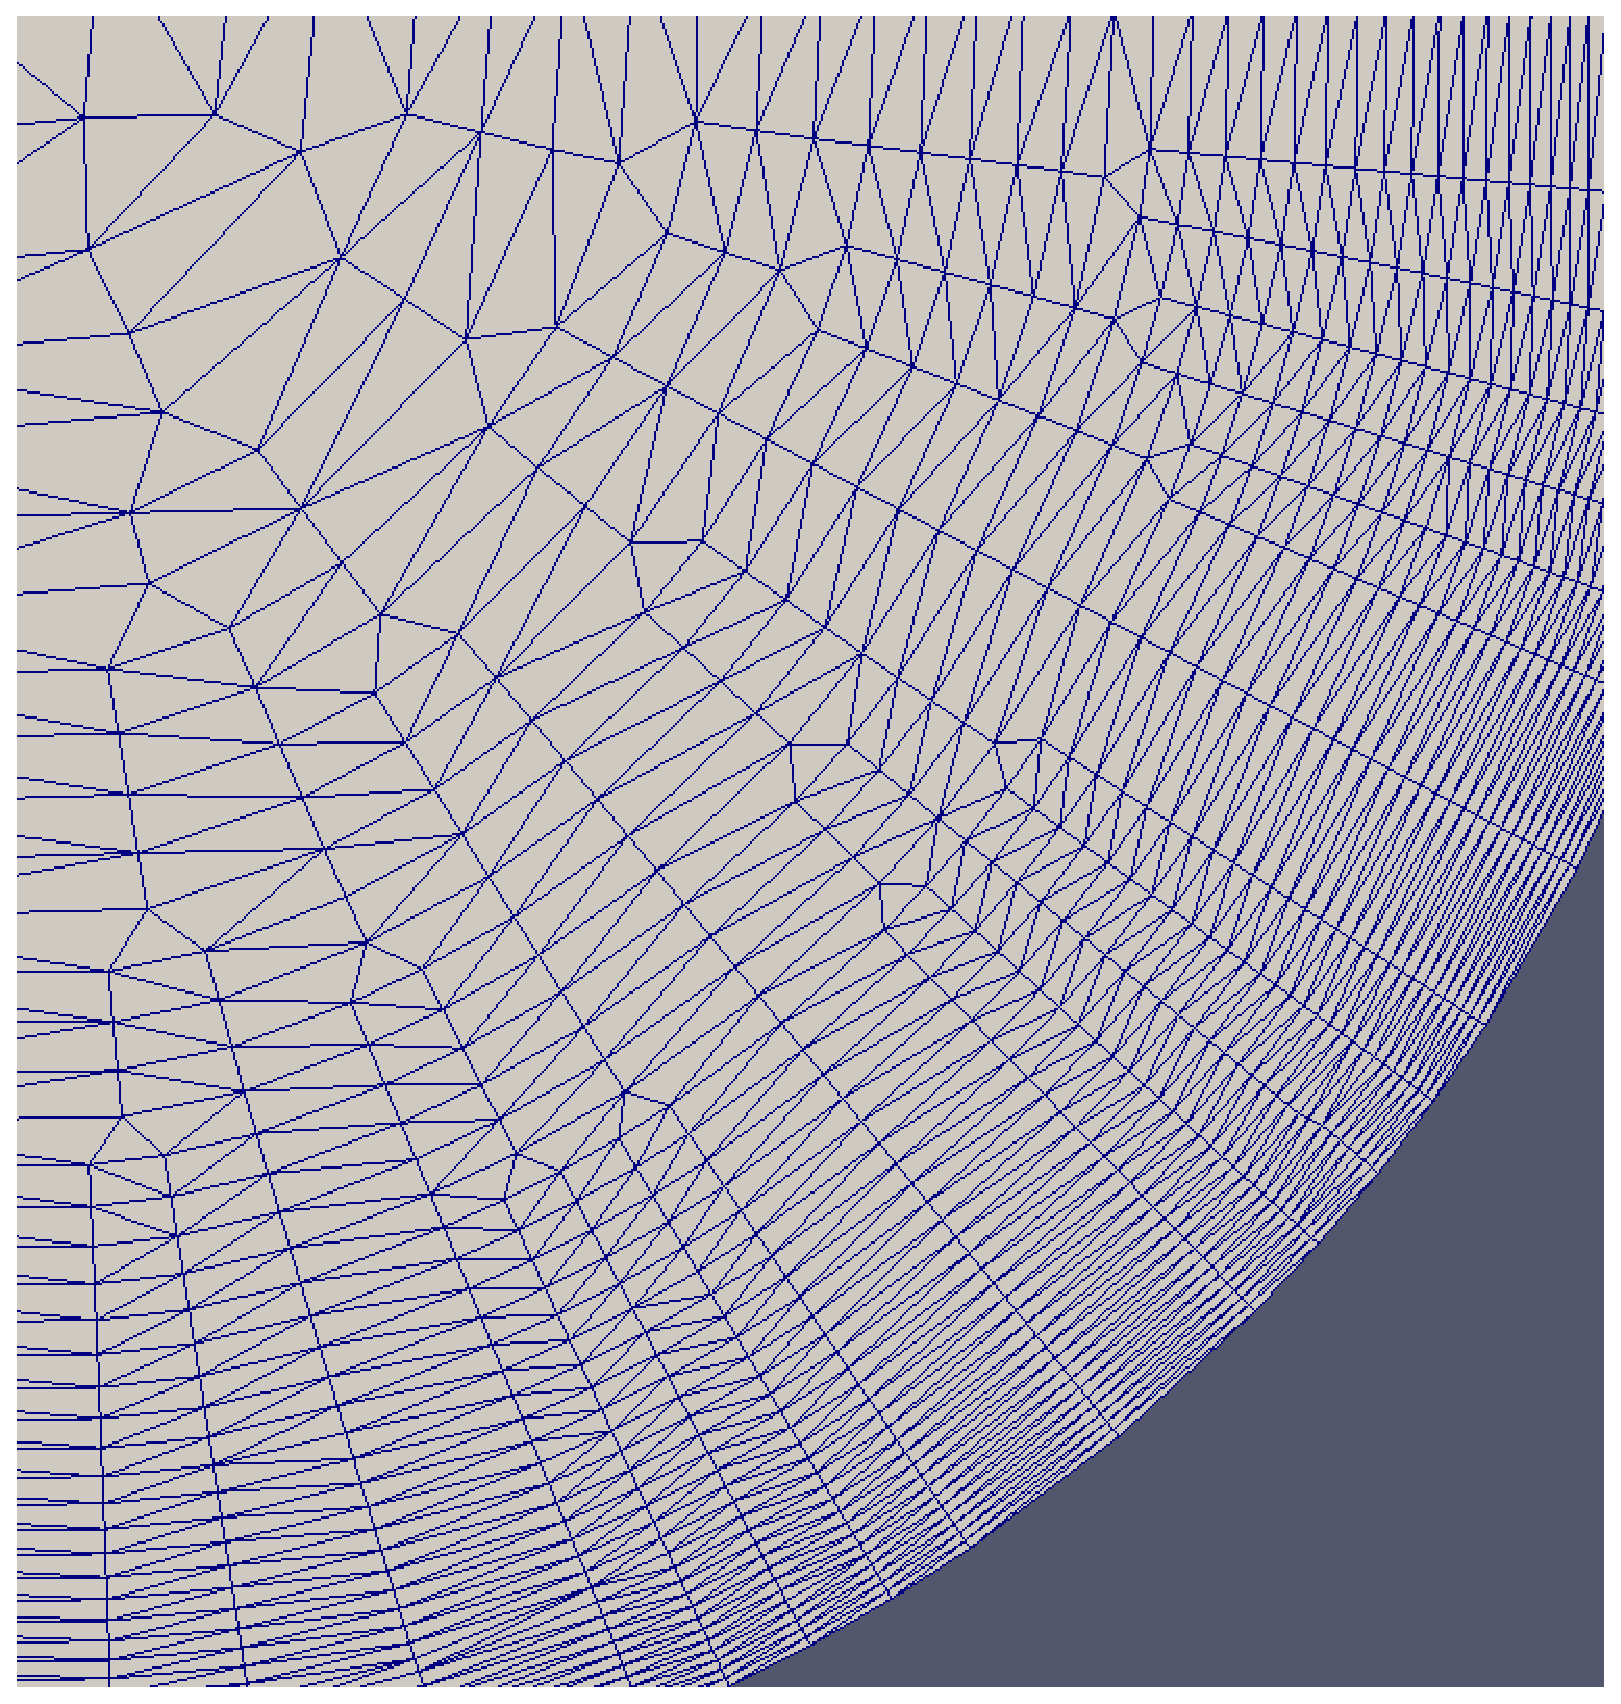
\includegraphics[width=0.9\linewidth]{img/m2/combine-tris-to-quads/combineTrisToQuads1.eps}
\caption{}
\label{fig-triQuad1}
\end{subfigure}%
\begin{subfigure}{0.5\textwidth}
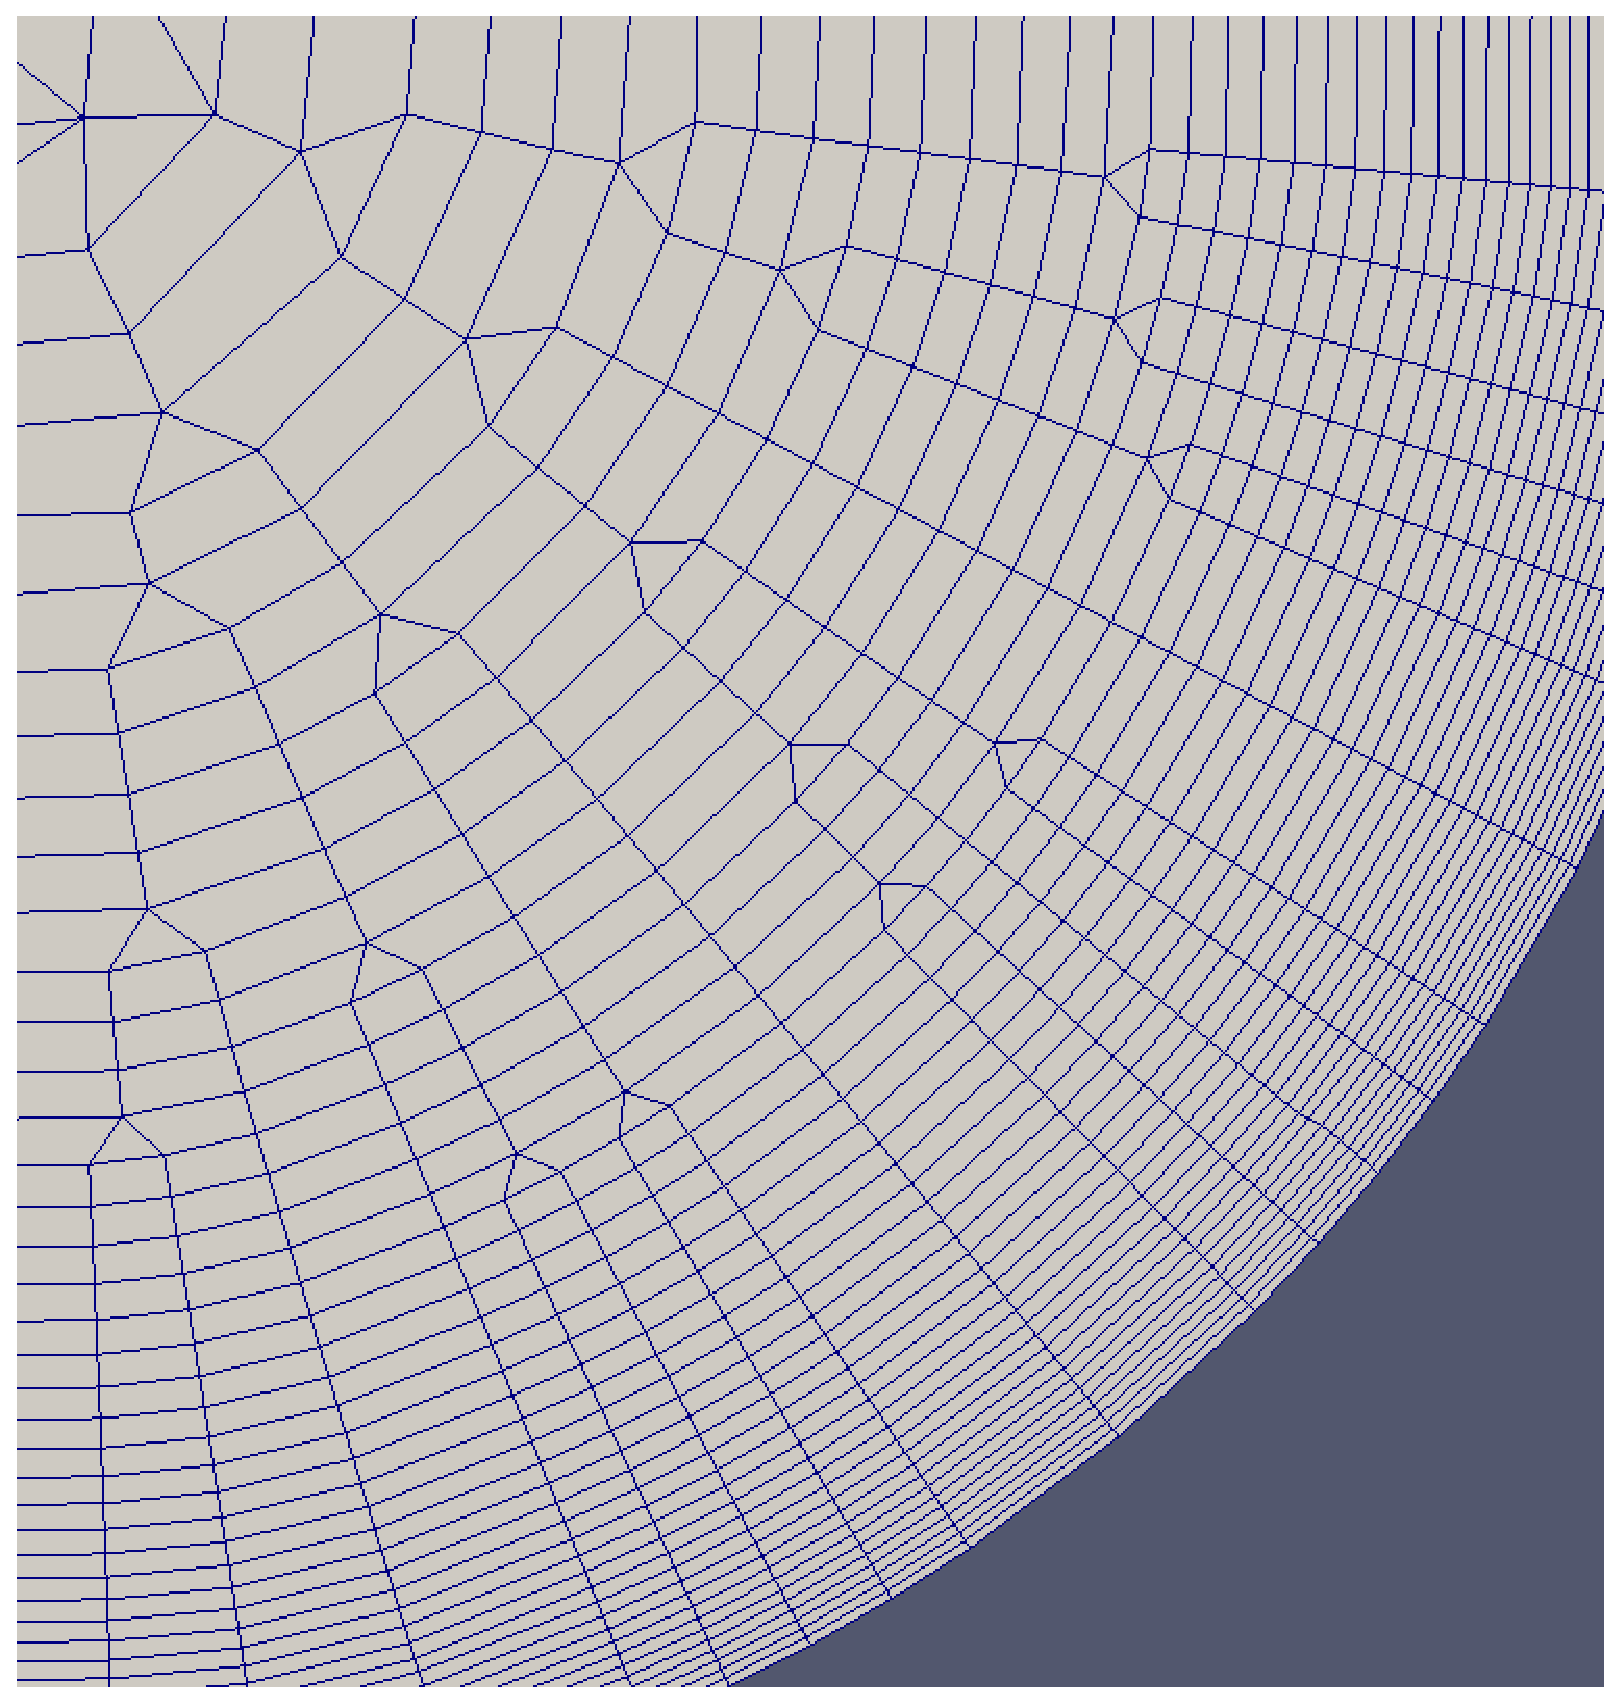
\includegraphics[width =0.9\linewidth]{img/m2/combine-tris-to-quads/combineTrisToQuads2.eps}
\caption{}
\label{fig-triQuad2}
\end{subfigure}
\caption{Combining triangular cells to quadrilateral cells based on the quality of the quadrilateral cells generated. For any given quadrilateral element, the inverse of the maximum deviation of its interior angles from 90$^\circ$ is adopted as the measure of quality.}
\label{fig-triQuad}
\end{figure}

\section{Mesh Smoothing}

Mesh smoothing is the process of improving the quality of the mesh. However, the context in which quality is referred to changes with the application of the mesh. Diffusion of mesh elements might be a desirable effect of mesh smoothing in one application and might not be a desirable effect in yet another application. One segment of the mesh smoothing techniques either proceed by filtering out noises of selected frequencies. Laplacian smoothing is the simplest example of such a smoothing technique. In a very simplistic Laplacian Smoothing technique, vertices on the mesh are moved towards the average position of its neighbours. Another implementation considers moving the centroid of an element towards the average location of the centroids of the adjacent elements. In either of the cases, there is a filteration of high frequency undulations on the surface mesh. This causes loss of sharp features on the surface. Also, such a smoothing methodology results in shrinkage of the volume of the geometry which might not be desirable everywhere.

Another segment of mesh smoothing methodology falls under the category of optimization by minimizing a given energy or error function in the mesh \cite{freitag1997tetrahedral, zhou2000angle, chen2004mesh, parthasarathy1991constrained, shephard1991automatic}. Here, a 

combined - \cite{freitag1997combining, canann1998approach}

For our mesh generation scheme, we choose a physically-based smoothing technique. The mesh vertices (or nodes) on the mesh exert forces on adjacent nodes. Subsequently, the mesh nodes move so as to balance out these forces and reach a local force balance equilibrium. This method of smoothing is also referred to as spring-based smoothing methodology as each edge (or link) in the mesh acts as a spring which pushes or pulls its end points away or towards each other.

Choosing a spring-based smoothing methodology gives us freedom to select the proportion of forces applied in the extrusion direction and along the advancing layer direction. The proportion can be changed by changing the spring constant of the springs associated with the edges in either direction. Several spring forces are applied to a given mesh node in the smoothing procedure. Each spring constant is denoted by $k_{spring}$. The forces are:


\begin{itemize}
\item \textbf{Parent force} - force which keeps the distance of the vertex to its parent (from which it was extruded) closer to the initial extrusion length, $\mathit{l_{ideal}}$ between the two.
\begin{equation}
\mathit{f_{parent}} = \mathit{k_{extrusion}} \cdot \frac{l_{real} - l_{ideal}}{l_{real} + l_{ideal}} \cdot \norm{ \vec{p} - \vec{v}}
\end{equation}
\item \textbf{Kid force} - similar to the parent force, this one keeps the distance between the node and its kid closer to the initial extrusion length.
\begin{equation}
\mathit{f_{kid} = k_{extrusion} * \frac{l_{real} - l_{ideal}}{l_{real} + l_{ideal}} * \norm{\vec{k} - \vec{v}}}
\end{equation}
\item \textbf{Neighbour force} - force to maintain uniform spacing of mesh nodes for each layer.
\begin{equation}
\mathit{f_{neighbour} = k_{neighbour} \cdot \frac{(\vec{v} - \vec{l}) + (\vec{v}- \vec{r})}{ 2.0}}
\end{equation}
\item \textbf{Original location} - a force is added to restrict the movement of the vertex from the location at which it was placed in the mesh before smoothing. This term also ensures that the deviation of the mesh nodes from the initial surface representation is as little as possible.
\begin{equation}
\mathit{f_{original} = k_{original} \cdot (\vec{v}- \vec{v'})}
\end{equation}
\end{itemize}

These forces are summed up to give the mesh node a resultant force and the node is moved according to the total force. Several iterations (around 5-10) of smoothing are done per layer as the mesh advances towards surface interior. A limit is set to the vertex movement per smoothing iteration. The distance a vertex moves per iteration of the smoothing algorithm is kept at $5\%$ of the extrusion length at that vertex. This helps in limiting the movement of the vertex when the initial boundary discretization is too coarse. The limitation of choosing a spring-based smoothing technique is that we have to carefully identify the spring constants, $\mathit{k_{spring}}$ for our algorithm. However, once these constants are identified, they seem to work reasonably well for all the cases that we run. The value of $\mathit{k_{extrusion}}$ we use is 0.01, $k_{neighbour}$ is kept at 0.02 and $\mathit{k_{original}}$ at 0.1. Figure \ref{fig-smoothing-cylinder} shows an advancing layer surface mesh with and without smoothing applied to the mesh vertices. It can be seen that smoothing helps improve the vertex spacing along the advancing layer, thereby making the aspect ratio more uniform at a given front.

\begin{figure}
\centering
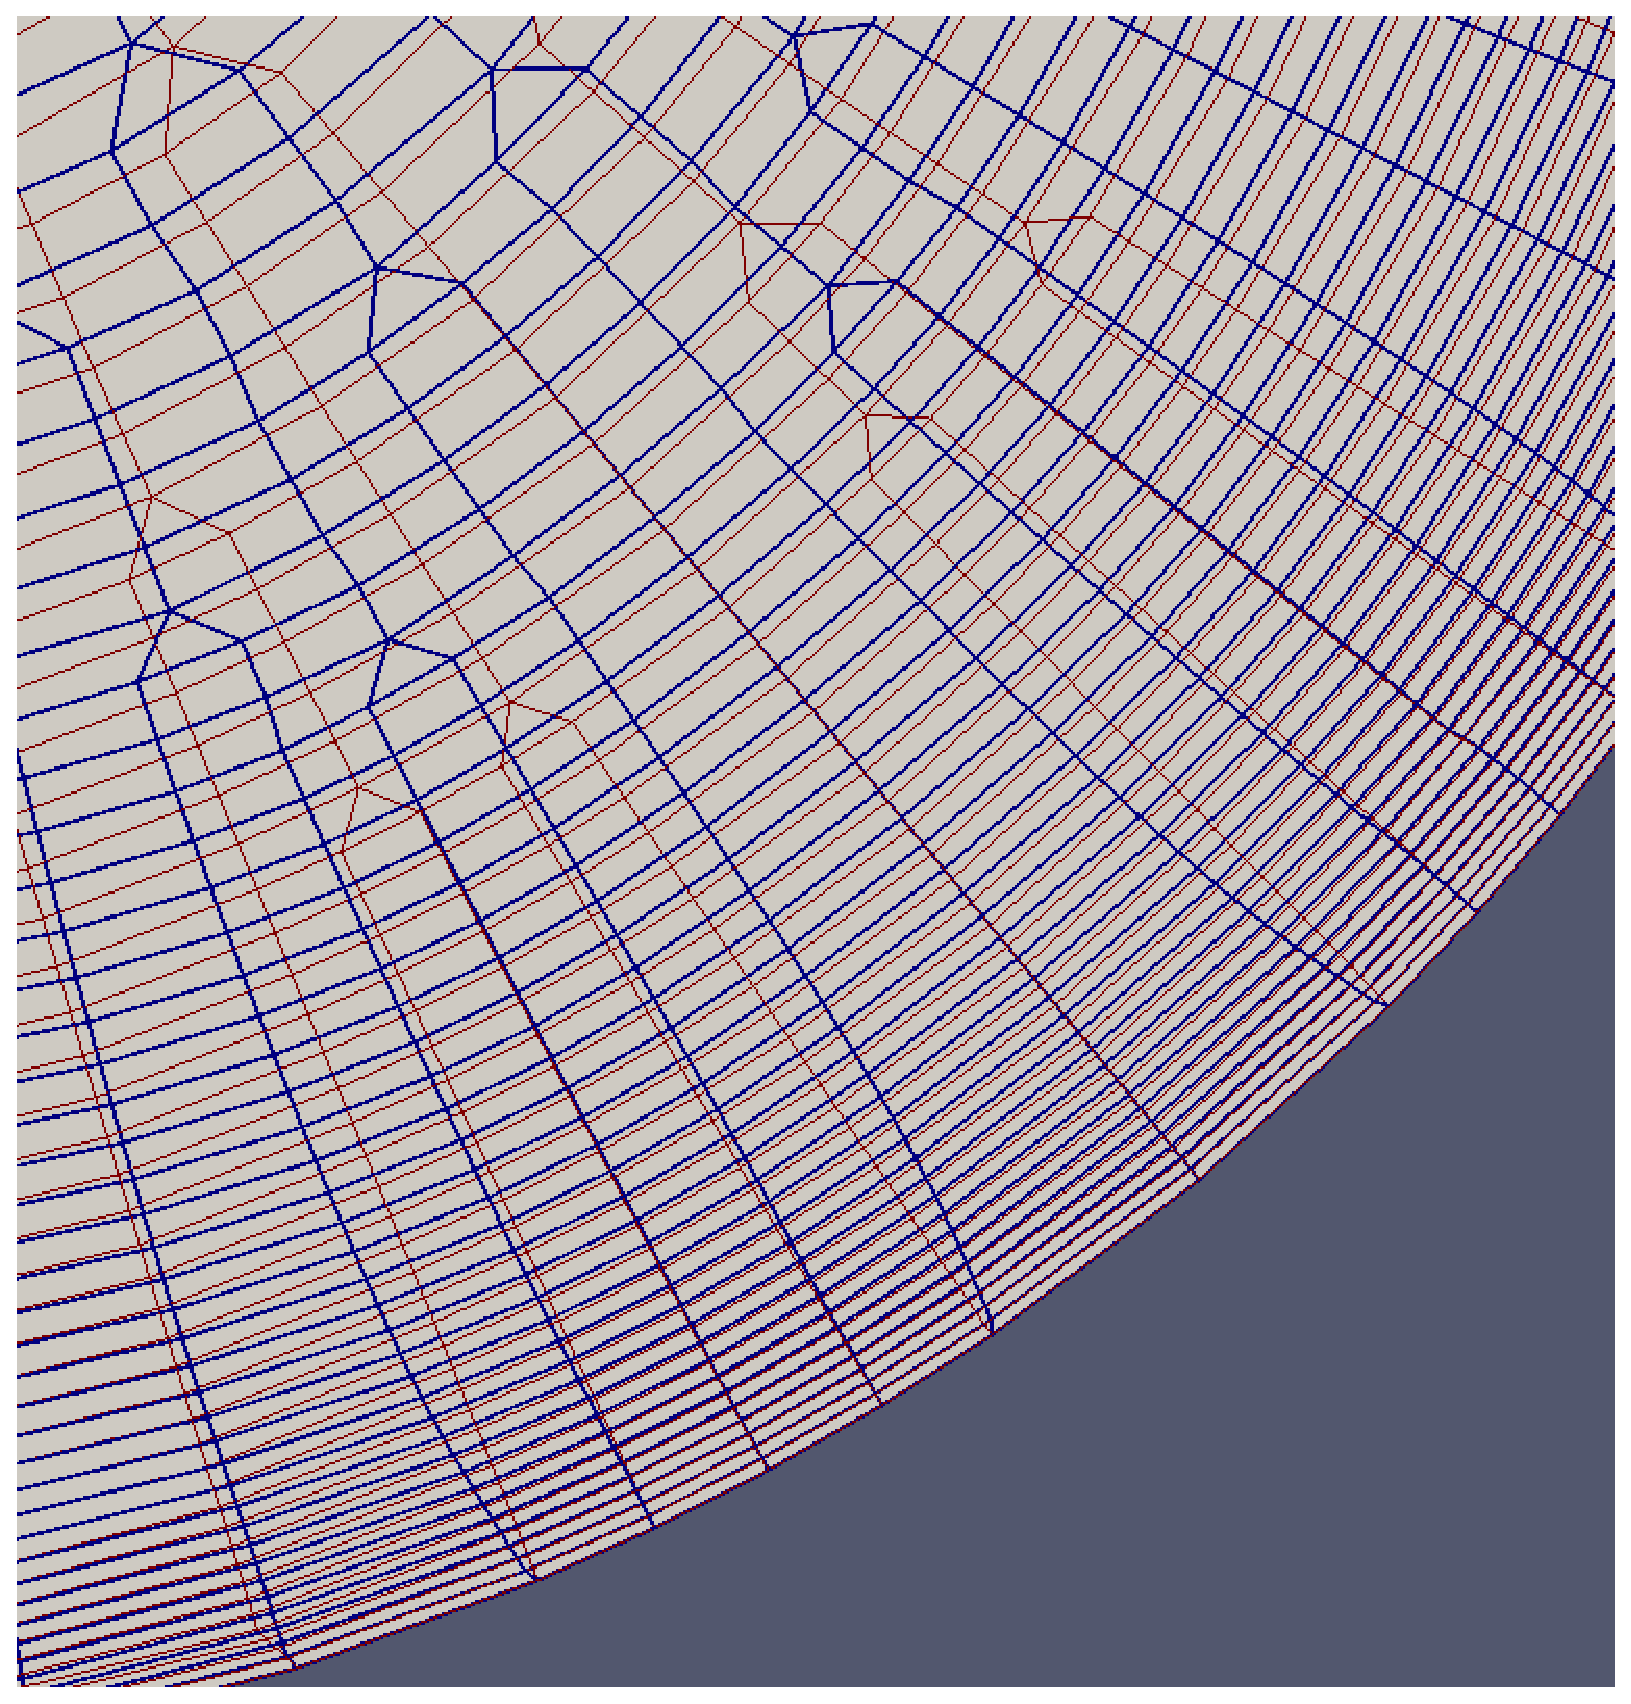
\includegraphics[width=0.4\linewidth]{img/m2/smoothing/smoothing-comparison-cylinder-cap.eps}
\caption{Zoomed in view of smoothing applied to an advancing layer surface mesh. Dark blue lines represent the smoothed mesh and flat red lines represent the mesh without smoothing. We can see that the smoothed version of the mesh helps to attain uniform aspect ratio at each layer.}
\label{fig-smoothing-cylinder}
\end{figure}

































%		4. Example Meshes
\chapter{Example Meshes}

In the first chapter, we gave a brief introduction to mesh generation. We discussed about structured, unstructured, simplical and non-simplical meshes and included a brief literature review of the research papers in the field of mesh generation. There, we stressed on the importance of generating anisotropic meshes or boundary layer meshes when solving for boundary layer phenomena and motivated the problem of generating stretched quad-dominant surface meshes to serve as the starting point of complete three dimensional anisotropic volume mesh generation.

We started discussing about the method we developed to generate such anisotropic quad-dominant meshes in the second chapter. Here, we discussed about the surface import, point placement, local reconnection and front recovery subroutines which are an essential part of the mesh generation process. In the third chapter, we discussed the subroutines used to advance several layers of the mesh and close off the marching layers so as to form a complete surface mesh. Controlling the aspect ratio on the advancing front, combining triangular elements to quadrilateral ones, mesh smoothing and collision handling were discussed.

In this chapter, we go over some of the example meshes generated by using EDAMSurf or Entire Domain Advancing Layer Mesh - Surface.

\section{NACA0018}

We take the NACA0018 airfoil 2D profile and extrude it in 3D. This gives us a three dimensional airfoil as shown in the figure.

%	5. Summary
\chapter{Summary}

\section{Concluding Comments}

In the field of Computational Fluid Dynamics, mesh generation and adaptation still takes considerable effort. It requires the mesh developer to have significant knowledge about the application of the mesh. This is more true in applications entailing boundary layer flows which requires a mesh with anisotropic or stretched elements. Creating valid anisotropic meshes for a diverse set of geometrical bodies is thus, a tedious and difficult task. Hence, some sort of automation in the development of anisotropic meshes will simplify the process of mesh generation for engineers and scientists. This thesis may represents one such step towards generating fully automatic anisotropic three-dimensional meshes.

Most of the three-dimensional anisotropic meshes start from the discretization of the surface. This discretization is generally an isotropic triangulation of the surface. In this thesis, we argue that an isotropic triangulation of the surface cannot be a foundation for completely anisotropic three-dimensional mesh. Hence, the mesh generation algorithm presented, called Entire Domain Advancing Layer Mesh Generation --- Surface (EDAMSurf), produces an anisotropic surface mesh from a given input triangulation of a solid body. The mesh generation algorithm initializes advancing fronts from the boundary curves of the surface patches of the input triangulation. The fronts advance layer-by-layer with the given growth ratio and sweep the surface of the geometry. Special subroutines are implemented to handle mesh smoothing, combining triangles to quadrilaterals, and to handle advancing front collisions.

EDAMSurf generates quad-dominant meshes with a few triangular elements. This is done to achieve low vertex connectivity in the mesh. Additionally, having non-simplicial elements in the mesh may lead to cancellation of local truncation errors while solving for fluid flows (See \ref{sec-simplicial}). The meshes generated by EDAMSurf generally have more than 95\% of the mesh elements as quadrilateral elements. Triangular elements are included in the mesh whenever there is a need to deal with complex corners or advancing layer collisions. Four example meshes that demonstrate the capabilities of the application are shown. The distribution of the interior angles of the mesh elements in the meshes generated by EDAMSurf show a peak at 90$^\circ$. This is because majority of mesh elements are rectangular in shape. Generally, mesh elements have more than 90\% of the angles in between 45$^\circ$ and 135$^\circ$. More triangular elements in the mesh give us more flattened angle distribution for the mesh elements.

EDAMSurf is shown to handle sharp concave corners in the input geometries well. It successfully retrieves advancing front definition while front collisions happen at the concave corners. The definition of the boundary curves is advanced several layers onto the surface mesh. Also, EDAMSurf is able to handle geometries with diverse topologies and holes. Example cases are demonstrated where multiple advancing layers collapse in a very small region and the mesh generation algorithm is able to successfully continue marching with a valid front definition.

\section{Future Work}

Automatic anisotropic meshing of complex three-dimensional domains is still a tricky task. EDAMSurf provides a step towards it, but is in no way a perfect one size fits all solution. EDAMSurf is a part of the project GRUMMP (Generation and Refinement of Unstructured Mixed-Element Meshes in Parallel)\cite{ollivier2010grummp} which is in continuous development. Some steps that might be taken in the future for improving and/or extending the mesh generation scheme are -

\begin{enumerate}
	\item EDAM3D is an extension of EDAMSurf. Being developed at ANSLab, UBC, it aims to develop completely anisotropic three-dimensional volume meshes for fluid flow applications.
	\item EDAMSurf handles concave corners robustly. Marching directions are eliminated when vertices on the advancing front collide with each other. In the future, a subroutine might be added to the algorithm which adds multiple marching directions to the convex corners of the surface so as to improve mesh quality.
	\item Due to the restrictions of Common Geometry Module's Application Programming Interface, EDAMSurf could not use curvature information on the imported surface to modify the marching direction as well as extrusion lengths on the front. A subroutine which is able to achieve this might allow EDAMSurf to tackle highly curved geometries with poor input discretization.
	\item EDAMSurf generates meshes of sub surfaces independently. Hence, a performance speedup could be attained by parallelising the application.
\end{enumerate}










%\include{relatedwork}
%\include{model}
%\include{impl}
%\include{discussion}
%\include{conclusions}

%    3. Notes
%    4. Footnotes

%    5. Bibliography
\begin{singlespace}
	\raggedright
	\bibliographystyle{abbrvnat}
	\bibliography{biblio}
\end{singlespace}

\appendix
%    6. Appendices (including copies of all required UBC Research
%       Ethics Board's Certificates of Approval)
%\include{reb-coa}	% pdfpages is useful here
%\chapter{Supporting Materials}

This would be any supporting material not central to the dissertation.
For example:
\begin{itemize}
\item additional details of methodology and/or data;
\item diagrams of specialized equipment developed.;
\item copies of questionnaires and survey instruments.
\end{itemize}


\backmatter
%    7. Index
% See the makeindex package: the following page provides a quick overview
% <http://www.image.ufl.edu/help/latex/latex_indexes.shtml>


\end{document}
